%**************************************%
%*    Generated from PreTeXt source   *%
%*    on 2017-09-26T12:31:15-07:00    *%
%*                                    *%
%*   http://mathbook.pugetsound.edu   *%
%*                                    *%
%**************************************%
\documentclass[10pt,openany,oneside]{book}
%% Custom Preamble Entries, early (use latex.preamble.early)
%% Inline math delimiters, \(, \), need to be robust
%% 2016-01-31:  latexrelease.sty  supersedes  fixltx2e.sty
%% If  latexrelease.sty  exists, bugfix is in kernel
%% If not, bugfix is in  fixltx2e.sty
%% See:  https://tug.org/TUGboat/tb36-3/tb114ltnews22.pdf
%% and read "Fewer fragile commands" in distribution's  latexchanges.pdf
\IfFileExists{latexrelease.sty}{}{\usepackage{fixltx2e}}
%% Text height identically 9 inches, text width varies on point size
%% See Bringhurst 2.1.1 on measure for recommendations
%% 75 characters per line (count spaces, punctuation) is target
%% which is the upper limit of Bringhurst's recommendations
%% Load geometry package to allow page margin adjustments
\usepackage{geometry}
\geometry{letterpaper,total={340pt,9.0in}}
%% Custom Page Layout Adjustments (use latex.geometry)
%% This LaTeX file may be compiled with pdflatex, xelatex, or lualatex
%% The following provides engine-specific capabilities
%% Generally, xelatex and lualatex will do better languages other than US English
%% You can pick from the conditional if you will only ever use one engine
\usepackage{ifthen}
\usepackage{ifxetex,ifluatex}
\ifthenelse{\boolean{xetex} \or \boolean{luatex}}{%
%% begin: xelatex and lualatex-specific configuration
%% fontspec package will make Latin Modern (lmodern) the default font
\ifxetex\usepackage{xltxtra}\fi
\usepackage{fontspec}
%% realscripts is the only part of xltxtra relevant to lualatex
\ifluatex\usepackage{realscripts}\fi
%%
%% Extensive support for other languages
\usepackage{polyglossia}
%% Main document language is US English
\setdefaultlanguage{english}
%% Spanish
\setotherlanguage{spanish}
%% Vietnamese
\setotherlanguage{vietnamese}
%% end: xelatex and lualatex-specific configuration
}{%
%% begin: pdflatex-specific configuration
%% translate common Unicode to their LaTeX equivalents
%% Also, fontenc with T1 makes CM-Super the default font
%% (\input{ix-utf8enc.dfu} from the "inputenx" package is possible addition (broken?)
\usepackage[T1]{fontenc}
\usepackage[utf8]{inputenc}
%% end: pdflatex-specific configuration
}
%% Monospace font: Inconsolata (zi4)
%% Sponsored by TUG: http://levien.com/type/myfonts/inconsolata.html
%% See package documentation for excellent instructions
%% One caveat, seem to need full file name to locate OTF files
%% Loads the "upquote" package as needed, so we don't have to
%% Upright quotes might come from the  textcomp  package, which we also use
%% We employ the shapely \ell to match Google Font version
%% pdflatex: "varqu" option produces best upright quotes
%% xelatex,lualatex: add StylisticSet 1 for shapely \ell
%% xelatex,lualatex: add StylisticSet 2 for plain zero
%% xelatex,lualatex: we add StylisticSet 3 for upright quotes
%%
\ifthenelse{\boolean{xetex} \or \boolean{luatex}}{%
%% begin: xelatex and lualatex-specific monospace font
\usepackage{zi4}
\setmonofont[BoldFont=Inconsolatazi4-Bold.otf,StylisticSet={1,3}]{Inconsolatazi4-Regular.otf}
%% end: xelatex and lualatex-specific monospace font
}{%
%% begin: pdflatex-specific monospace font
\usepackage[varqu]{zi4}
%% end: pdflatex-specific monospace font
}
%% Symbols, align environment, bracket-matrix
\usepackage{amsmath}
\usepackage{amssymb}
%% allow page breaks within display mathematics anywhere
%% level 4 is maximally permissive
%% this is exactly the opposite of AMSmath package philosophy
%% there are per-display, and per-equation options to control this
%% split, aligned, gathered, and alignedat are not affected
\allowdisplaybreaks[4]
%% allow more columns to a matrix
%% can make this even bigger by overriding with  latex.preamble.late  processing option
\setcounter{MaxMatrixCols}{30}
%%
%% Color support, xcolor package
%% Always loaded.  Used for:
%% mdframed boxes, add/delete text, author tools
\PassOptionsToPackage{usenames,dvipsnames,svgnames,table}{xcolor}
\usepackage{xcolor}
%%
%% Semantic Macros
%% To preserve meaning in a LaTeX file
%% Only defined here if required in this document
%% Used for warnings, typically bold and italic
\newcommand{\alert}[1]{\textbf{\textit{#1}}}
%% Used for inline definitions of terms
\newcommand{\terminology}[1]{\textbf{#1}}
%% Subdivision Numbering, Chapters, Sections, Subsections, etc
%% Subdivision numbers may be turned off at some level ("depth")
%% A section *always* has depth 1, contrary to us counting from the document root
%% The latex default is 3.  If a larger number is present here, then
%% removing this command may make some cross-references ambiguous
%% The precursor variable $numbering-maxlevel is checked for consistency in the common XSL file
\setcounter{secnumdepth}{3}
%% Environments with amsthm package
%% Theorem-like environments in "plain" style, with or without proof
\usepackage{amsthm}
\theoremstyle{plain}
%% Numbering for Theorems, Conjectures, Examples, Figures, etc
%% Controlled by  numbering.theorems.level  processing parameter
%% Always need a theorem environment to set base numbering scheme
%% even if document has no theorems (but has other environments)
\newtheorem{theorem}{Theorem}[section]
%% Only variants actually used in document appear here
%% Style is like a theorem, and for statements without proofs
%% Numbering: all theorem-like numbered consecutively
%% i.e. Corollary 4.3 follows Theorem 4.2
\newtheorem{corollary}[theorem]{Corollary}
\newtheorem{lemma}[theorem]{Lemma}
%% Definition-like environments, normal text
%% Numbering is in sync with theorems, etc
\theoremstyle{definition}
\newtheorem{definition}[theorem]{Definition}
%% Remark-like environments, normal text
%% Numbering is in sync with theorems, etc
\theoremstyle{definition}
\newtheorem{remark}[theorem]{Remark}
\newtheorem{convention}[theorem]{Convention}
\newtheorem{note}[theorem]{Note}
\newtheorem{observation}[theorem]{Convention}
\newtheorem{warning}[theorem]{Warning}
%% Example-like environments, normal text
%% Numbering is in sync with theorems, etc
\theoremstyle{definition}
\newtheorem{example}[theorem]{Example}
%% Miscellaneous environments, normal text
%% Numbering for inline exercises and lists is in sync with theorems, etc
\theoremstyle{definition}
\newtheorem{exercise}[theorem]{Exercise}
%% Localize LaTeX supplied names (possibly none)
\renewcommand*{\proofname}{Proof}
\renewcommand*{\appendixname}{Appendix}
\renewcommand*{\chaptername}{Chapter}
%% Equation Numbering
%% Controlled by  numbering.equations.level  processing parameter
\numberwithin{equation}{section}
%% For improved tables
\usepackage{array}
%% Some extra height on each row is desirable, especially with horizontal rules
%% Increment determined experimentally
\setlength{\extrarowheight}{0.2ex}
%% Define variable thickness horizontal rules, full and partial
%% Thicknesses are 0.03, 0.05, 0.08 in the  booktabs  package
\makeatletter
\newcommand{\hrulethin}  {\noalign{\hrule height 0.04em}}
\newcommand{\hrulemedium}{\noalign{\hrule height 0.07em}}
\newcommand{\hrulethick} {\noalign{\hrule height 0.11em}}
%% We preserve a copy of the \setlength package before other
%% packages (extpfeil) get a chance to load packages that redefine it
\let\oldsetlength\setlength
\newlength{\Oldarrayrulewidth}
\newcommand{\crulethin}[1]%
{\noalign{\global\oldsetlength{\Oldarrayrulewidth}{\arrayrulewidth}}%
\noalign{\global\oldsetlength{\arrayrulewidth}{0.04em}}\cline{#1}%
\noalign{\global\oldsetlength{\arrayrulewidth}{\Oldarrayrulewidth}}}%
\newcommand{\crulemedium}[1]%
{\noalign{\global\oldsetlength{\Oldarrayrulewidth}{\arrayrulewidth}}%
\noalign{\global\oldsetlength{\arrayrulewidth}{0.07em}}\cline{#1}%
\noalign{\global\oldsetlength{\arrayrulewidth}{\Oldarrayrulewidth}}}
\newcommand{\crulethick}[1]%
{\noalign{\global\oldsetlength{\Oldarrayrulewidth}{\arrayrulewidth}}%
\noalign{\global\oldsetlength{\arrayrulewidth}{0.11em}}\cline{#1}%
\noalign{\global\oldsetlength{\arrayrulewidth}{\Oldarrayrulewidth}}}
%% Single letter column specifiers defined via array package
\newcolumntype{A}{!{\vrule width 0.04em}}
\newcolumntype{B}{!{\vrule width 0.07em}}
\newcolumntype{C}{!{\vrule width 0.11em}}
\makeatother
%% Figures, Tables, Listings, Floats
%% The [H]ere option of the float package fixes floats in-place,
%% in deference to web usage, where floats are totally irrelevant
%% We re/define the figure, table and listing environments, if used
%%   1) New mbxfigure and/or mbxtable environments are defined with float package
%%   2) Standard LaTeX environments redefined to use new environments
%%   3) Standard LaTeX environments redefined to step theorem counter
%%   4) Counter for new environments is set to the theorem counter before caption
%% You can remove all this figure/table setup, to restore standard LaTeX behavior
%% HOWEVER, numbering of figures/tables AND theorems/examples/remarks, etc
%% WILL ALL de-synchronize with the numbering in the HTML version
%% You can remove the [H] argument of the \newfloat command, to allow flotation and
%% preserve numbering, BUT the numbering may then appear "out-of-order"
\usepackage{float}
\usepackage[bf]{caption} % http://tex.stackexchange.com/questions/95631/defining-a-new-type-of-floating-environment
\usepackage{newfloat}
% Figure environment setup so that it no longer floats
\SetupFloatingEnvironment{figure}{fileext=lof,placement={H},within=section,name=Figure}
% figures have the same number as theorems: http://tex.stackexchange.com/questions/16195/how-to-make-equations-figures-and-theorems-use-the-same-numbering-scheme
\makeatletter
\let\c@figure\c@theorem
\makeatother
% Table environment setup so that it no longer floats
\SetupFloatingEnvironment{table}{fileext=lot,placement={H},within=section,name=Table}
% tables have the same number as theorems: http://tex.stackexchange.com/questions/16195/how-to-make-equations-figures-and-theorems-use-the-same-numbering-scheme
\makeatletter
\let\c@table\c@theorem
\makeatother
%% Footnote Numbering
%% We reset the footnote counter, as given by numbering.footnotes.level
\makeatletter\@addtoreset{footnote}{section}\makeatother
%% Raster graphics inclusion, wrapped figures in paragraphs
%% \resizebox sometimes used for images in side-by-side layout
\usepackage{graphicx}
%%
%% Program listing support, for inline code, Sage code
\usepackage{listings}
%% We define the listings font style to be the default "ttfamily"
%% To fix hyphens/dashes rendered in PDF as fancy minus signs by listing
%% http://tex.stackexchange.com/questions/33185/listings-package-changes-hyphens-to-minus-signs
\makeatletter
\lst@CCPutMacro\lst@ProcessOther {"2D}{\lst@ttfamily{-{}}{-{}}}
\@empty\z@\@empty
\makeatother
\ifthenelse{\boolean{xetex}}{}{%
%% begin: pdflatex-specific listings configuration
%% translate U+0080 - U+00F0 to their textmode LaTeX equivalents
%% Data originally from https://www.w3.org/Math/characters/unicode.xml, 2016-07-23
%% Lines marked in XSL with "$" were converted from mathmode to textmode
\lstset{extendedchars=true}
\lstset{literate={ }{{~}}{1}{¡}{{\textexclamdown }}{1}{¢}{{\textcent }}{1}{£}{{\textsterling }}{1}{¤}{{\textcurrency }}{1}{¥}{{\textyen }}{1}{¦}{{\textbrokenbar }}{1}{§}{{\textsection }}{1}{¨}{{\textasciidieresis }}{1}{©}{{\textcopyright }}{1}{ª}{{\textordfeminine }}{1}{«}{{\guillemotleft }}{1}{¬}{{\textlnot }}{1}{­}{{\-}}{1}{®}{{\textregistered }}{1}{¯}{{\textasciimacron }}{1}{°}{{\textdegree }}{1}{±}{{\textpm }}{1}{²}{{\texttwosuperior }}{1}{³}{{\textthreesuperior }}{1}{´}{{\textasciiacute }}{1}{µ}{{\textmu }}{1}{¶}{{\textparagraph }}{1}{·}{{\textperiodcentered }}{1}{¸}{{\c{}}}{1}{¹}{{\textonesuperior }}{1}{º}{{\textordmasculine }}{1}{»}{{\guillemotright }}{1}{¼}{{\textonequarter }}{1}{½}{{\textonehalf }}{1}{¾}{{\textthreequarters }}{1}{¿}{{\textquestiondown }}{1}{À}{{\`{A}}}{1}{Á}{{\'{A}}}{1}{Â}{{\^{A}}}{1}{Ã}{{\~{A}}}{1}{Ä}{{\"{A}}}{1}{Å}{{\AA }}{1}{Æ}{{\AE }}{1}{Ç}{{\c{C}}}{1}{È}{{\`{E}}}{1}{É}{{\'{E}}}{1}{Ê}{{\^{E}}}{1}{Ë}{{\"{E}}}{1}{Ì}{{\`{I}}}{1}{Í}{{\'{I}}}{1}{Î}{{\^{I}}}{1}{Ï}{{\"{I}}}{1}{Ð}{{\DH }}{1}{Ñ}{{\~{N}}}{1}{Ò}{{\`{O}}}{1}{Ó}{{\'{O}}}{1}{Ô}{{\^{O}}}{1}{Õ}{{\~{O}}}{1}{Ö}{{\"{O}}}{1}{×}{{\texttimes }}{1}{Ø}{{\O }}{1}{Ù}{{\`{U}}}{1}{Ú}{{\'{U}}}{1}{Û}{{\^{U}}}{1}{Ü}{{\"{U}}}{1}{Ý}{{\'{Y}}}{1}{Þ}{{\TH }}{1}{ß}{{\ss }}{1}{à}{{\`{a}}}{1}{á}{{\'{a}}}{1}{â}{{\^{a}}}{1}{ã}{{\~{a}}}{1}{ä}{{\"{a}}}{1}{å}{{\aa }}{1}{æ}{{\ae }}{1}{ç}{{\c{c}}}{1}{è}{{\`{e}}}{1}{é}{{\'{e}}}{1}{ê}{{\^{e}}}{1}{ë}{{\"{e}}}{1}{ì}{{\`{\i}}}{1}{í}{{\'{\i}}}{1}{î}{{\^{\i}}}{1}{ï}{{\"{\i}}}{1}{ð}{{\dh }}{1}{ñ}{{\~{n}}}{1}{ò}{{\`{o}}}{1}{ó}{{\'{o}}}{1}{ô}{{\^{o}}}{1}{õ}{{\~{o}}}{1}{ö}{{\"{o}}}{1}{÷}{{\textdiv }}{1}{ø}{{\o }}{1}{ù}{{\`{u}}}{1}{ú}{{\'{u}}}{1}{û}{{\^{u}}}{1}{ü}{{\"{u}}}{1}{ý}{{\'{y}}}{1}{þ}{{\th }}{1}{ÿ}{{\"{y}}}{1}}
%% end: pdflatex-specific listings configuration
}
%% End of generic listing adjustments
%% Inline code, typically from "c" element
%% Global, document-wide options apply to \lstinline
%% Search/replace \lstinline by \verb to remove this dependency
%% (redefining \lstinline with \verb is unlikely to work)
%% Also see "\renewcommand\UrlFont" below for matching font choice
\lstset{basicstyle=\small\ttfamily,breaklines=true,breakatwhitespace=true,extendedchars=true,inputencoding=latin1}
%% Multiple column, column-major lists
\usepackage{multicol}
%% More flexible list management, esp. for references and exercises
%% But also for specifying labels (i.e. custom order) on nested lists
\usepackage{enumitem}
%% Lists of references in their own section, maximum depth 1
\newlist{referencelist}{description}{4}
\setlist[referencelist]{leftmargin=!,labelwidth=!,labelsep=0ex,itemsep=1.0ex,topsep=1.0ex,partopsep=0pt,parsep=0pt}
%% Lists of exercises in their own section, maximum depth 4
\newlist{exerciselist}{description}{4}
\setlist[exerciselist]{leftmargin=0pt,itemsep=1.0ex,topsep=1.0ex,partopsep=0pt,parsep=0pt}
%% Package for tables spanning several pages
\usepackage{longtable}
%% hyperref driver does not need to be specified, it will be detected
\usepackage{hyperref}
%% configure hyperref's  \url  to match listings' inline verbatim
\renewcommand\UrlFont{\small\ttfamily}
%% Hyperlinking active in PDFs, all links solid and blue
\hypersetup{colorlinks=true,linkcolor=blue,citecolor=blue,filecolor=blue,urlcolor=blue}
\hypersetup{pdftitle={First-Semester Abstract Algebra}}
%% If you manually remove hyperref, leave in this next command
\providecommand\phantomsection{}
%% Graphics Preamble Entries
\usepackage[all]{xy}
\usepackage{pgfplots}
%% If tikz has been loaded, replace ampersand with \amp macro
\ifdefined\tikzset
    \tikzset{ampersand replacement = \amp}
\fi
%% NB: calc redefines \setlength
\usepackage{calc}
%% used repeatedly for vertical dimensions of sidebyside panels
\newlength{\panelmax}
%% extpfeil package for certain extensible arrows,
%% as also provided by MathJax extension of the same name
%% NB: this package loads mtools, which loads calc, which redefines
%%     \setlength, so it can be removed if it seems to be in the
%%     way and your math does not use:
%%
%%     \xtwoheadrightarrow, \xtwoheadleftarrow, \xmapsto, \xlongequal, \xtofrom
%%
%%     we have had to be extra careful with variable thickness
%%     lines in tables, and so also load this package late
\usepackage{extpfeil}
%% Custom Preamble Entries, late (use latex.preamble.late)
%% Begin: Author-provided packages
%% (From  docinfo/latex-preamble/package  elements)
%% End: Author-provided packages
%% Begin: Author-provided macros
%% (From  docinfo/macros  element)
%% Plus three from MBX for XML characters
\def\Z{\mathbb{Z}}
\def\zn{\mathbb{Z}_n}
\def\znc{\mathbb{Z}_n^\times}
\def\R{\mathbb{R}}
\def\Q{\mathbb{Q}}
\def\C{\mathbb{C}}
\def\N{\mathbb{N}}
\def\M{\mathbb{M}}
\def\G{\mathcal{G}}
\def\0{\mathbf 0}
\def\Gdot{\langle G, \cdot\,\rangle}
\def\phibar{\overline{\phi}}
\DeclareMathOperator{\lcm}{lcm}
\DeclareMathOperator{\Ker}{Ker}
\def\siml{\sim_L}
\def\simr{\sim_R}
\newcommand{\lt}{<}
\newcommand{\gt}{>}
\newcommand{\amp}{&}
%% End: Author-provided macros
%% Title page information for book
\title{First-Semester Abstract Algebra\\
{\large A Structural Approach}}
\author{Jessica K. Sklar\\
Department of Mathematics\\
Pacific Lutheran University\\
\href{mailto:sklarjk@plu.edu}{\nolinkurl{sklarjk@plu.edu}}
}
\date{}
\begin{document}
\frontmatter
%% begin: half-title
\thispagestyle{empty}
{\centering
\vspace*{0.28\textheight}
{\Huge First-Semester Abstract Algebra}\\[2\baselineskip]
{\LARGE A Structural Approach}\\
}
\clearpage
%% end:   half-title
%% begin: adcard
\thispagestyle{empty}
\null%
\clearpage
%% end:   adcard
%% begin: title page
%% Inspired by Peter Wilson's "titleDB" in "titlepages" CTAN package
\thispagestyle{empty}
{\centering
\vspace*{0.14\textheight}
%% Target for xref to top-level element is ToC
\addtocontents{toc}{\protect\hypertarget{fsaa}{}}
{\Huge First-Semester Abstract Algebra}\\[\baselineskip]
{\LARGE A Structural Approach}\\[3\baselineskip]
{\Large Jessica K. Sklar}\\[0.5\baselineskip]
{\Large Pacific Lutheran University}\\}
\clearpage
%% end:   title page
%% begin: copyright-page
\thispagestyle{empty}
\vspace*{\stretch{2}}
\noindent{\bfseries Edition}: First Edition\par\medskip
\noindent\textcopyright\ 2017\quad{}Jessica K. Sklar\\[0.5\baselineskip]
Permission is granted to copy, distribute and/or modify this document under the terms of the GNU Free Documentation License, Version 1.3 or any later version published by the Free Software Foundation; with no Invariant Sections, no Front-Cover Texts, and no Back-Cover Texts.  A copy of the license is included in the appendix entitled ``GNU Free Documentation License.''\par\medskip
\vspace*{\stretch{1}}
\null\clearpage
%% end:   copyright-page
%% begin: acknowledgement
\chapter*{Acknowledgements}\label{acknowledgement-1}
\addcontentsline{toc}{chapter}{Acknowledgements}
Thank you to Jennifer Nordstrom of Linfield College for introducing me to the \href{http://mathbook.pugetsound.edu}{PreTeXt} authoring system; to Rob Beezer at the University of Puget Sound for facilitating my entry into the PreTeXt world;  to David Farmer at the \href{https://aimath.org/textbooks/}{Open Textbook Initiative} for typesetting the initial draft of this book in PreTeXt; and to Rob, David, Mitch Keller, Alex Jordan, Bob Plantz, Alex Best, and everyone else otheir extensive technical help via the \href{https://groups.google.com/forum/?fromgroups\#!forum/pretext-support}{PreTeXt support} group.%
%% end:   acknowledgement
%% begin: preface
\chapter*{Preface}\label{preface-1}
\addcontentsline{toc}{chapter}{Preface}
\alert{A note on rendering:} If you are accessing the HTML version of this book, please be patient; the mathematical content may take a minute to load. If you see what appears to be strange code, or a box at the bottom of your screen saying \lstinline?Processing Math: 0%?, just give the page a little time to fully load.%
\par
\alert{A note on algebra:} At its most basic level, abstract algebra is the study of structures. Just as an architect may examine buildings or an anthropologist societal hierarchies, an algebraist explores the nature of sets equipped with binary operations that satisfy certain properties. While these structures may not seem at first to be very important, they are at the heart of most, if not all, mathematical endeavors. On an elemental level, they allow us to solve systems of equations; on a more global-level, they are behind some of our most important cryptographic systems. We even use them implicitly when telling time!%
\par
Our focus in this course will be exploring some of the most fundamental algebraic structures: namely, groups, rings, and fields. Along the way, we will explore rigorous mathematical notions of similarity and difference: When can we consider two objects to be more or less ``the same''? When are they fundamentally different? For instance, consider two houses that have exactly the same construction, but are painted different colors. Are they the same house? No. But viewed structurally (as opposed to aesthetically) they are the same. This means that if we know certain information about one of the houses (say, how far the bathroom is from the kitchen) we know the same information about the other house. However, knowing that the first house is painted yellow does not tell us anything about the second house's color. We explore an analogous idea in mathematics, namely, the concept of \emph{isomorphism}.%
\par
Along the way, we will gain experience writing mathematical proofs and will see plenty of specific examples demonstrating more general ideas.%
%% end:   preface
%% begin: table of contents
%% Adjust Table of Contents
\setcounter{tocdepth}{1}
\renewcommand*\contentsname{Contents}
\tableofcontents
%% end:   table of contents
\mainmatter
\typeout{************************************************}
\typeout{Chapter 1 Preliminaries}
\typeout{************************************************}
\chapter[{Preliminaries}]{Preliminaries}\label{pre}
\typeout{************************************************}
\typeout{Section 1.1 Sets}
\typeout{************************************************}
\section[{Sets}]{Sets}\label{section-1}
We start off by providing a ``definition'' of a basic mathematical structure to which we will soon add bells and whistles. We use quotes here because what follows doesn't have the precision we usually require when defining a mathematical object.%
\begin{definition}[{}]\label{definition-1}
A \terminology{set} is an (unordered) collection of objects.%
\end{definition}
This is only sort of  a ``definition'' because it is not a rigorous definition of a set. For instance, what do we mean by a ``collection'' of objects? This ``definition'' will be sufficient for our course, but be warned that defining a set in this vague way can lead to some serious mathematical issues, such as \emph{Russell's paradox}.  A mathematician whose expertise is in set theory may scowl disagreeably if you try to define a set as we have above.%
\begin{note}[]\label{note-1}
Let \(S\) be the set of all sets that aren't members of themselves.  Is \(S\) a member of itself? If you think carefully about this, you'll see that \(S\) can be neither a member of itself, nor \emph{not} a member of itself. Uh oh!  This contradiction is known as ``Russell's paradox'' (named for the British philosopher, mathematician, and all-round academic Bertrand Russell). Mathematicians deal with this by declaring that some object collections, called \emph{classes}, are not in fact sets.%
\end{note}
\begin{definition}[{}]\label{definition-2}
\label{notation-1}
\label{notation-2}
\label{notation-3}
The members of a set are called its \terminology{elements}. If \(S\) is a set, we write \(x\in S\) to indicate ``\(x\) is an element of \(S\),'' and \(x \not\in S\) to indicate ``\(x\) is not an element of \(S\).'' There is a unique set containing no elements; it is called the \terminology{empty set}, and denoted by \(\emptyset\).%
\end{definition}
Sets must be \emph{well defined}: that is, it must be clear exactly which objects are in a set, and which objects aren't. For instance, the set of all integers is well defined, but the set of all big integers is not well defined, since it is unclear what ``big'' means in this context.%
\par
We refer to some sets so frequently in mathematics that we have special notation for them.%
\begin{example}[]\label{example-1}
\label{notation-4}
 \label{notation-5}
 \label{notation-6}
 \label{notation-7}
 \label{notation-8}
 \label{notation-9}
 \label{notation-10}
 \label{notation-11}
Some common sets are: \leavevmode%
\begin{description}
\item[{\(\Z\)}]\hypertarget{li-1}{}the set of all integers  (the \(\Z\) comes ``zahlen,'' the German word for ``numbers'')%
\item[{\(\Q\)}]\hypertarget{li-2}{}set of all rational numbers%
\item[{\(\R\)}]\hypertarget{li-3}{}the set of all real numbers%
\item[{\(\C\)}]\hypertarget{li-4}{}the set of all complex numbers%
\item[{\(\N\)}]\hypertarget{li-5}{}the set of all natural numbers, i.e., \(\{0, 1, 2, \ldots\}\)%
\par
(Be aware that many books/mathematicians do not include \(0\) in the set of natural numbers%
\end{description}
 We can further write denote by \(\Z^+\) the set of all positive integers, and by \(\Z^*\) the set of all nonzero integers. Can you guess what the penultimate notation represents if we replace \(\Z\) with \(\Q\) or \(\R\), and/or \(+\) with \(-\)? What about what the last notation, if we replace \(\Z\) with \(\Q\), \(\R\), or \(\C\)?%
\end{example}
We also provide notation for commonly considered sets of matrices:%
\begin{definition}[{}]\label{definition-3}
\label{notation-12}
\label{notation-13}
Given \(m,n\in \Z^+\) and a set \(S\), we define \(\M_{m\times n}(S)\) to be the set of all \(m\times n\) matrices over \(S\) (that is, of all \(m\times n\) matrices with entries in \(S\)). We use the shorthand notation \(\M_n(S)\) for the set \(\M_{n\times n}(S)\).%
\end{definition}
One common way of describing a set is to list its elements in curly braces, separated by commas; you can use ellipses to indicate a repeated pattern of elements. A few examples are \(\{1,4,\pi\}\), \(\{3, 4, 5, \ldots\}\), and \(\{\ldots, -4, -2, 0,
2, 4, \ldots\}\); the last of these can be written more concisely as \(\{0,\pm 2, \pm 4,\ldots\}\). Note that since elements of a set are unordered, the sets \(\{1,4,\pi\}\) and \(\{4,\pi, 1\}\), for instance, are identical.%
\par
Another method is using \terminology{set-builder notation}. This consists of an element name (or names), followed by a colon (meaning ``such that''), followed by a Boolean expression involving the element name(s), all surrounded by curly braces.%
\begin{warning}[]\label{warning-1}
The use of a colon to denote ``such that'' is \emph{only} valid in the above set-builder notation context.  Outside of this context, you should never use a colon to denote ``such that''; instead, use the abbreviation ``s.t.'' or write out the actual words.   Conversely, never use one of those ways of indicating ``such that'' within set-builder notation; always use a colon there.  Why?  Convention.%
\end{warning}
For example,%
\begin{equation*}
\{x\in \Z : x > 4\}
\end{equation*}
is the set \(\{5, 6, 7, \ldots\}\), while%
\begin{equation*}
\{z\in \C : |z|=1\}
\end{equation*}
is the set of all complex numbers at distance 1 from the origin in the complex plane.%
\begin{note}[]\label{note-2}
If one simply writes \(\{x\,:\,x>4\}\), it is unclear what this set is; it could be the set of all integers greater than 4, or the set of all real numbers greater than 4, or something else. When one can, it is better to identify the named element(s) as a member (members) of a known set, such as \(\R\) or \(\Z\), whenever possible.%
\end{note}
\begin{definition}[{}]\label{definition-4}
\label{notation-14}
\label{notation-15}
Set \(A\) is a \terminology{subset} of \(B\) (and set \(B\) is a \terminology{superset} of \(A\)) if every element in \(A\) is also in \(B\). We denote ``\(A\) is a subset of \(B\)'' by \(A\subseteq B\). Sets \(A\) and \(B\) are said to be \terminology{equal}, and we write \(A=B\), if they contain exactly the same elements; equivalently, \(A=B\) if and only if \(A \subseteq B\) and \(B\subseteq A\). Set \(A\) is a \terminology{proper} subset of set \(B\) if \(A\subseteq B\) but \(A\neq B\); we write this \(A\subsetneq B\).%
\end{definition}
\begin{remark}[]\label{remark-1}
Sometimes the notation \(A\subset B\) is  used to indicate that \(A\) is a proper subset of \(B\), and sometimes it is simply used to mean that \(A\) is a subset\textemdash{}proper or improper\textemdash{}of \(B\). We will not use the notation \(A \subset B\) in this text.%
\end{remark}
\begin{note}[]\label{note-3}
One often proves that two sets \(A\) and \(B\) are equal by proving that \(A\subseteq B\) and \(B\subseteq A\).%
\end{note}
\begin{example}[]\label{example-2}
We have the following: \(\Z^+ \subseteq \Z \subseteq \Q \subseteq \R \subseteq \C\).%
\end{example}
\begin{definition}[{}]\label{definition-5}
\label{notation-16}
The \terminology{power set} of \(A\), denoted \(P(A)\), is the set of all subsets of \(A\). (Note that the power set of any set contains the empty set as an element.)%
\end{definition}
\begin{warning}[]\label{warning-2}
Be careful to use your curly braces correctly when writing power sets! Remember, the power set of a set is a \emph{set of sets}.%
\end{warning}
The following provides a good example of using braces correctly.%
\begin{example}[]\label{example-3}
If \(A=\{a,b\}\), then \(P(A)=\{\emptyset, \{a\}, \{b\}, \{a,b\}\}\). Note that the element \(\{a,b\}\) of \(P(A)\) could also be written simply as \(A\).%
\end{example}
\begin{definition}[{}]\label{definition-6}
\label{notation-17}
\label{notation-18}
\label{notation-19}
\label{notation-20}
\label{notation-21}
\leavevmode%
\begin{enumerate}
\item\hypertarget{li-6}{}If \(A\) and \(B\) are sets, then the \terminology{union} of \(A\) and \(B\), denoted \(A\cup B\), is the set \(A\cup B=\{x: x\in A \text{ or }  x\in B\};\) the \terminology{intersection} of \(A\) and \(B\), denoted \(A\cap B\), is the set \(A\cap B=\{x: x\in A \text{ and }  x\in B\};\) and the \terminology{difference} of \(A\) and \(B\), denoted \(A-B\) (or \(A\setminus B\)), is the set \(A-B=\{x: x\in A \text{ and }  x\not\in B\}.\)%
\item\hypertarget{li-7}{}More generally, given any collection of sets \(A_i\) (\(i\) in some index set \(I\)), the \terminology{union} of the \(A_i\) is%
\begin{equation*}
\bigcup_{i\in I}A_i=\{x: x\in A_i \text{ for some }  i\in I\},
\end{equation*}
and the \terminology{intersection} of the \(A_i\) is%
\begin{equation*}
\bigcap_{i\in I}A_i=\{x: x\in A_i \text{ for every }  i\in I\}.
\end{equation*}
%
\item\hypertarget{li-8}{}Sets \(A\) and \(B\) are \emph{disjoint} if \(A\cap B=\emptyset\).  More generally, sets \(A_i\) (\(i\) in some index set \(I\)) are \emph{disjoint} if%
\begin{equation*}
\bigcap_{i\in I}A_i=\emptyset
\end{equation*}
and are \emph{mutually disjoint} if%
\begin{equation*}
A_i\cap A_j=\emptyset \text{ for all } i\neq j \in I.
\end{equation*}
%
\end{enumerate}
%
\end{definition}
Notice that for any sets \(A\) and \(B\), \(A\cap B \subseteq A \subseteq A\cup B\) and \(A\cap B \subseteq B \subseteq A\cup B\). Also note that if sets \(A_i\) (\(i \in I\)) are mutually disjoint then they are also disjoint, but they may be disjoint without being mutually disjoint. For example, the sets \(\{i, i+1\}\) for \(i\in \Z\) are disjoint but not mutually disjoint. (Do you see why?)%
\par
We define one more way of ``combining'' sets.%
\begin{definition}[{}]\label{definition-7}
\label{notation-22}
Let \(A\) and \(B\) be sets. Then the \terminology{direct product} (or \terminology{Cartesian product}) \(A\times B\) of \(A\) and \(B\) is the set%
\begin{equation*}
A\times B =\{(a,b): \text{\(a\in A\), \(b\in B\)} \}.
\end{equation*}
%
\par
An element \((a,b)\) of \(A\times B\) is called an \terminology{ordered pair}. More generally, if \(A_1, A_2, \ldots, A_n\) are sets for some \(n\in \Z^+\), then the \terminology{product} of the \(A_i\) is%
\begin{equation*}
A_1\times A_2 \times \cdots \times A_n=\{(a_1, a_2 \ldots, a_n): a_i \in A_i \text{ for
} i=1,2, \ldots, n\};
\end{equation*}
the elements \((a_1,a_2,\ldots,a_n)\) of this product are called \(n\)-tuples (or triples, if \(n=3\)). (You can also have products of infinitely many sets, but we will not discuss that in this course.) Finally, if each set \(A_i\) is the same set \(A\), we can use the notation \(A^n\) to denote the product%
\begin{equation*}
A\times A \times \cdots \times A
\end{equation*}
of \(n\) copies of \(A\).%
\end{definition}
\begin{example}[]\label{example-4}
For example, the Cartesian plane is the set \(\R^2\), and the set \(\Z \times \R\) consists of exactly the points in the plane with integer \(x\)-coordinates (that is, the points that lie on vertical lines intersecting the \(x\)-axis at integer values).%
\end{example}
\typeout{************************************************}
\typeout{Section 1.2 Functions}
\typeout{************************************************}
\section[{Functions}]{Functions}\label{section-2}
You have probably encountered functions before. In introductory calculus, for instance, you typically deal with functions from \(\R\) to \(\R\) (e.g., the function \(f(x)=x^2\)). More generally, functions ``send'' elements of one set to elements of another set; these sets may or may not be sets of real numbers. We provide below a ``good enough for government work'' definition of a function.%
\begin{definition}[{}]\label{definition-8}
\label{notation-23}
\label{notation-24}
\label{notation-25}
A \terminology{function} \(f\) from a set \(S\) to a set \(T\) is a ``rule'' that assigns to each element \(s\) in \(S\) a unique element \(f(s)\) in \(T\); the element \(f(s)\) is called the \terminology{image of \(s\) under \(f\)}. If \(f\) is a function from \(S\) to \(T\), we write \(f: S \to T\), and call \(S\) the \terminology{domain} of \(f\) and \(T\) the \terminology{codomain} of \(f\). The \terminology{range} of \(f\) is%
\begin{equation*}
f(S)=\{f(s) \in T : s \in S\} \subseteq T.
\end{equation*}
%
\par
More generally, if \(U \subseteq S\), the \terminology{image of \(U\) in \(T\) under \(f\)} is%
\begin{equation*}
f(U)=\{f(u)\in T : u\in U\}.
\end{equation*}
%
\par
If \(V\subseteq T\), the \terminology{preimage of \(V\) in \(S\) under \(f\)} is the set%
\begin{equation*}
f^{\leftarrow}(V)=\{s\in S: f(s)\in V\}.
\end{equation*}
%
\end{definition}
\begin{example}[]\label{example-5}
Consider the function \(f: \Z \to \R\) defined by \(f(x)=x^2\). The domain of \(f\) is \(\Z\) and the codomain of \(f\) is \(\R\); the range of \(f\) is \(\{x^2\,:\,x\in \Z\}=\{0,1,4,9,\ldots\}\). The image of \(\{-2,-1,1,2\}\) under \(f\) is the two-element set \(\{1,4\} \subseteq
\R\), and the preimage of \(\{4,25,\pi\}\) under \(f\) is the set \(\{\pm 2, \pm 5\}\). (Do you see why \(\pm \sqrt{\pi}\) are not in this preimage?) What is the preimage of just \(\{\pi\}\) under \(f\)?%
\end{example}
The following definitions will be very important in our future work.%
\begin{definition}[{}]\label{definition-9}
Let \(S\) and \(T\) be sets, and \(f:S\to T\). \leavevmode%
\begin{enumerate}
\item\hypertarget{li-9}{}Function \(f\) is \terminology{one-to-one} (1-1) if whenever \(s_1, s_2\in S\) with \(f(s_1)=f(s_2)\), we have \(s_1=s_2\).  Equivalently, \(f\) is one-to-one if whenever \(s_1\neq s_2 \in S\), then \(f(s_1)\neq f(s_2) \in T\).%
\item\hypertarget{li-10}{}Function \(f\) is \terminology{onto} if for every \(t\in T\), there exists an element \(s\in S\) such that \(f(s)=t\).  Equivalently, \(f\) is onto if \(f(S)=T\).%
\item\hypertarget{li-11}{}Function \(f\) is a \terminology{bijection} if it is both one-to-one and onto.%
\end{enumerate}
%
\end{definition}
\begin{remark}[]\label{remark-2}
We will often have to show functions are one-to-one or onto. Given a function \(f:S\to T\), the following methods are recommended. \leavevmode%
\begin{itemize}[label=\textbullet]
\item{}To prove that \(f\) is one-to-one: Let \(s_1,s_2 \in S\) with \(f(s_1)=f(s_2)\) and prove that then \(s_1=s_2\).%
\par
\alert{Note: It is \emph{not} sufficient to prove that if \(s_1=s_2\) in \(S\) then \(f(s_1)=f(s_2)\); that holds true for ANY function from \(S\) to \(T\)!  Be careful to \emph{assume} and \emph{prove} the correct facts.}%
\item{}To prove that \(f\) is \emph{not} one-to-one: Identify two elements \(s_1 \neq s_2\) of \(S\) such that \(f(s_1)=f(s_2)\).%
\item{}To prove that \(f\) is onto: Let \(t\in T\) and prove that there exists an element \(s\in S\) with \(f(s)=t\).%
\par
\alert{Note: It is \emph{not} sufficient to prove that if \(s\in S\) then \(f(s)\) is in \(T\); that holds true for ANY function from \(S\) to \(T\)!  Again, be careful to \emph{assume} and \emph{prove} the correct facts.}%
\item{}To prove that \(f\) is \emph{not} onto: Identify an element \(t\in T\) for which there is no \(s\in S\) with \(f(s)=t\).%
\end{itemize}
%
\end{remark}
\begin{example}[]\label{example-6}
Consider the function \(f: \R^* \to \R^+\) defined by \(f(x)=x^2\). Function \(f\) is \emph{not} one-to-one: indeed, \(-1\) and \(1\) are in \(\R^*\) with \(f(-1)=1=f(1)\) in \(\R^+\). However, \(f\) \emph{is} onto: indeed, let \(t\in \R^+\). Then \(\sqrt{t} \in \R^*\) with \(t=f(\sqrt{t})\), so we're done.%
\end{example}
\begin{example}[]\label{example-7}
Consider the function \(f: \Z^+ \to \R\) defined by \(f(x)=x/2\). Function \(f\) \emph{is} one-to-one: indeed, let \(s_1, s_2 \in \Z^+\) with \(f(s_1)=f(s_2)\). Then \(s_1/2=f(s_1)=f(s_2)=s_2/2\); multiplying both sides of the equation \(s_1/2=s_2/2\) by 2, we obtain \(s_1=s_2\). However, \(f\) is \emph{not} onto: for example, \(\pi\in \R\) but there is no positive integer \(s\) for which \(f(s)=s/2=\pi\).%
\end{example}
Recall that we can combine certain functions using \emph{composition}:%
\begin{definition}[{}]\label{definition-10}
\label{notation-26}
\label{notation-27}
If \(f:S\to T\) and \(g:T\to U\), then the  \terminology{composition of \(f\) and \(g\)} is the function \(g\circ f: S\to U\) defined by%
\begin{equation*}
(g\circ f)(s)=g(f(s))
\end{equation*}
for all \(s\in S\). (More generally, you can \terminology{compose} functions \(f:S\to T\) and \(g:R\to U\) to form \(g\circ f:S\to U\),  as long as \(f(S)\subseteq R\).) Also recall that given any set \(S\), the \emph{identity function on \(S\)} is the function \(1_S: S\to S\) defined by \(1_S(s)=s\) for every \(s\in S\).%
\end{definition}
\begin{definition}[{}]\label{definition-11}
Let \(f\) be a function from \(S\) to \(T\). A function \(g\) from \(T\) to \(S\) is an \terminology{inverse} of \(f\) if \(g\circ f\) and \(f\circ g\) are the identity functions on \(S\) and \(T\), respectively; that is, if for all \(s\in S\) and \(t\in
T\), \(g(f(s))=s\) and \(f(g(t))=t\).%
\par
We say a function is \terminology{invertible} if it has an inverse.%
\end{definition}
We have the following useful theorems.%
\begin{theorem}[{}]\label{invbij}
Function \(f:S\to T\) is invertible if and only if \(f\) is a bijection.%
\end{theorem}
\begin{proof}\hypertarget{proof-1}{}
Suppose \(f\) has inverse \(g\). Let \(t\in T\). Then \(f(g(t))=t\), so \(f\) is onto.  Next, suppose \(s_1,s_2\in S\) with \(f(s_1)=f(s_2)\). Then%
\begin{equation*}
s_1=g(f(s_1))=g(f(s_2))=s_2,
\end{equation*}
so \(f\)is one-to-one.%
\par
Conversely, suppose \(f\) is a bijection.  Then for every \(t\in T\), there exists a unique element \(s_t\in S\) such that \(f(s_t)=t\). It is then straighforward to show that the function \(g:T\to S\) defined by%
\begin{equation*}
g(t)=t_s \text{ for every }t\in T
\end{equation*}
is an inverse of \(f\).%
\end{proof}
\begin{theorem}[{}]\label{theorem-2}
\label{notation-28}
 Let \(f:S\to T\) be invertible. Then the  inverse of \(f\) is unique; we denote the unique inverse of \(f\) by \(f^{-1}\).%
\end{theorem}
\begin{proof}\hypertarget{proof-2}{}
Suppose \(f\) has inverses \(g\) and \(h\). Then for every \(t\in T,\) \(f(g(t))=t=f(h(t))\). But since \(f\) is invertible, it's one-to-one, so we must have \(g(t)=h(t)\) for every \(t\in T\). Thus, \(g=h\), and so \(f\) cannot have two or more distinct inverses.%
\end{proof}
\begin{theorem}[{}]\label{compbij}
Let \(f:S\to T\) and \(g:T\to U\) be functions. If \(f\) and \(g\) are both 1-1 [onto], then so is \(g\circ f: S\to U\).%
\end{theorem}
\begin{proof}\hypertarget{proof-3}{}
Assume \(f\) and \(g\) are 1-1. Let \(s_1, s_2\in S\) with \((g\circ f)(s_1)=(g\circ f)(s_2)\). Then \(g(f(s_1))=g(f(s_2))\); since \(g\) is one-to-one (since it's a bijection), this shows that \(f(s_1)=f(s_2)\). Then since \(f\) is one-to-one (since \(f\) is also a bijection), we must have \(s_1=s_2\). Thus, \(g\circ f\) is one-to-one.%
\par
The proof that \(g\circ f\) is onto if \(f\) and \(g\) are onto is left as an exercise for the reader.%
\end{proof}
\typeout{************************************************}
\typeout{Section 1.3 Cardinality}
\typeout{************************************************}
\section[{Cardinality}]{Cardinality}\label{section-3}
One of the set traits that will be useful to us in distinguishing between algebraic structures is \emph{cardinality}.%
\begin{definition}[{}]\label{definition-12}
\label{notation-29}
 A set is \terminology{finite} if it contains a finite number of elements; otherwise, it's \terminology{infinite}. The \terminology{cardinality} of a finite set \(S\) is the number of elements in \(S\); we denote the cardinality of \(S\) by \(|S|\).%
\end{definition}
\begin{warning}[]\label{warning-3}
Of course, vertical bars are used to denote other mathematical concepts; for instance, if \(x\) is a real number, \(|x|\) usually denotes the absolute value of \(x\). You must determine from context, and from the nature of the expression within the bars, what vertical bars mean in a particular context.%
\end{warning}
Note that in the above definition, we omitted the definition of the cardinality of an infinite set.  This is because defining the cardinality of an infinite set is a more complicated endeavor, and one which is, in the most general context, beyond the scope of this class.  For us it will suffice to distinguish between two types of infinite sets: \emph{countably infinite} sets and \emph{uncountable} (or \emph{uncountably infinite}) sets.%
\begin{definition}[{}]\label{definition-13}
A set \(S\) is said to be \terminology{countably infinite} if there exists a bijection from \(S\) to \(\Z\) (equivalently, if there exists a bijection from \(\Z\) to \(S\)). It is said to be \terminology{countable} if it is finite or countably infinite, and \terminology{uncountable} (or \terminology{uncountably infinite}) if it is not countable.%
\end{definition}
Here are some straightforward examples to get us started:%
\begin{example}[]\label{example-8}
\leavevmode%
\begin{enumerate}
\item\hypertarget{li-16}{}\(|\{a,b\}|=2\).%
\item\hypertarget{li-17}{}\(|\emptyset|=0\).%
\item\hypertarget{li-18}{}Clearly, \(\Z\) itself is countably infinite.%
\end{enumerate}
%
\end{example}
\begin{remark}[]\label{remark-3}
It turns out that countably infinite sets have the same cardinality as one another, while a countably infinite set and an uncountable set have different cardinalities. Intuitively, you  can think  of two countably infinite sets as having the same ``size,'' and a countable set and an uncountable set as having different ``sizes''; however, this is a risky way of framing things, since it can  make some results seem counterintuitive when you're used to dealing only with finite sets (see, for instance, \hyperref[zplus]{Example~6}).  Luckily, exploring the cardinality of infinite sets isn't the focus of this class.%
\end{remark}
Perhaps surprisingly, a proper subset of a set can have the same cardinality as its superset, as the following example shows.%
\begin{example}[]\label{zplus}
We claim that \(\Z^+\) is countably infinite. Indeed, consider the function \(f:\Z^+ \to \Z\) defined by \(f(n)=(-1)^n \lfloor n/2 \rfloor\), where \(\lfloor x \rfloor\) denotes the greatest integer less than or equal to \(x\), for each \(x\in \R\). The fact that \(f\) is a bijection is demonstrated (though not proven) by the following visual representation, where each number maps via \(f\) to the value directly to the right of it:%
% group protects changes to lengths, releases boxes (?)
{% begin: group for a single side-by-side
% set panel max height to practical minimum, created in preamble
\setlength{\panelmax}{0pt}
\newsavebox{\panelboxAtabular}
\savebox{\panelboxAtabular}{%
\raisebox{\depth}{\parbox{1\linewidth}{\centering\begin{tabular}{rr}
\(1\)&\(0\)\tabularnewline[0pt]
\(1\)&\(1\)\tabularnewline[0pt]
\(2\)&\(-1\)\tabularnewline[0pt]
\(3\)&\(2\)\tabularnewline[0pt]
\(4\)&\(-2\)\tabularnewline[0pt]
\(\vdots\)&\(\vdots\)
\end{tabular}
}}}
\newlength{\phAtabular}\setlength{\phAtabular}{\ht\panelboxAtabular+\dp\panelboxAtabular}
\settototalheight{\phAtabular}{\usebox{\panelboxAtabular}}
\setlength{\panelmax}{\maxof{\panelmax}{\phAtabular}}
\leavevmode%
% begin: side-by-side as tabular
% \tabcolsep change local to group
\setlength{\tabcolsep}{0\linewidth}
% @{} suppress \tabcolsep at extremes, so margins behave as intended
\par\medskip\noindent
\begin{tabular}{@{}*{1}{c}@{}}
\begin{minipage}[c][\panelmax][t]{1\linewidth}\usebox{\panelboxAtabular}\end{minipage}\end{tabular}\\
% end: side-by-side as tabular
}% end: group for a single side-by-side
\par
Note that this means that \(\Z\) and its proper subset \(\Z^+\) have the same cardinality, that is, the same ``size''!%
\end{example}
We summarize here examples of countably and uncountably infinite sets. (On pp. 5\textendash{}6 of~\hyperlink{F}{[1]}, Fraleigh sketches proofs of the facts that \(\Q\) is countable and that the interval \((0,1)\) in \(\R\) is uncountable. The proof then that \(\R\) is uncountable follows from \hyperref[cardthm]{Theorem~7}, below.)%
\par
Countably infinite sets: \(\Z\), \(\Z^+\), \(\Z^-\), \(\Z^*\), \(\Q\), \(\Q^+\), \(\Q^-\), \(\Q^*\), \(\N\)%
\par
Uncountably infinite sets: \(\R\), \(\R^+\), \(\R^-\), \(\R^*\), \(\C\), \(\C^*\),  the interval \((0,1)\) in \(\R\)%
\par
The key idea here for us is that if two sets are essentially ``the same,'' then they must have the same ``size.'' Thus, we see that there is some fundamental difference between the sets \(\Z\) and \(\R\) (in fact, there are many such differences). On the other hand, cardinality alone won't allow us to distinguish structurally between the sets \(\Z\) and \(\Z^+\).%
\par
We end our preliminary chapter with the following theorem and a corollary of it (which can be proved using induction on \(n\)). We prove only the fourth statement in the theorem, omitting the proofs of the first two statements and leaving the proof of the third statement as an exercise for the reader.%
\begin{theorem}[{}]\label{cardthm}
Let \(A\) and \(B\) be sets. \leavevmode%
\begin{enumerate}
\item\hypertarget{li-19}{}If \(A\subseteq B\) and \(A\) is infinite [uncountable] then so is \(B\).%
\item\hypertarget{li-20}{}If \(A\subseteq B\) and \(B\) is finite [countable] then so is \(A\).%
\item\hypertarget{li-21}{}If \(|A|=n\lt \infty\) and \(|B|=m\lt  \infty\), then \(|A\times B|=mn\).%
\item\hypertarget{li-22}{}Any finite product of countable sets is countable.%
\end{enumerate}
%
\end{theorem}
\begin{proof}\hypertarget{proof-4}{}
To prove the fourth statement: Let \(A\) and \(B\) be countable sets. Assume that \(A\) and \(B\) are both countably infinite. Since \(\Z^+\) is countably infinite, we can index the elements of \(A\) and of \(B\) by \(\Z^+\), writing%
\begin{equation*}
A=\{a_1,a_2,\ldots\} \text{ and }  B=\{b_1,b_2,\ldots\}.
\end{equation*}
%
\par
Notice that the table%
% group protects changes to lengths, releases boxes (?)
{% begin: group for a single side-by-side
% set panel max height to practical minimum, created in preamble
\setlength{\panelmax}{0pt}
\newsavebox{\panelboxBtabular}
\savebox{\panelboxBtabular}{%
\raisebox{\depth}{\parbox{1\linewidth}{\centering\begin{tabular}{llll}
\((a_1,b_1)\)&\((a_1,b_2)\)&\((a_1,b_3)\)&\(\cdots\)\tabularnewline[0pt]
\((a_2,b_1)\)&\((a_2,b_2)\)&\((a_2,b_3)\)&\(\cdots\)\tabularnewline[0pt]
\((a_3,b_1)\)&\((a_3,b_2)\)&\((a_3,b_3)\)&\(\cdots\)\tabularnewline[0pt]
\(\vdots\)&\(\vdots\)&\(\vdots\)&\(\ddots\)
\end{tabular}
}}}
\newlength{\phBtabular}\setlength{\phBtabular}{\ht\panelboxBtabular+\dp\panelboxBtabular}
\settototalheight{\phBtabular}{\usebox{\panelboxBtabular}}
\setlength{\panelmax}{\maxof{\panelmax}{\phBtabular}}
\leavevmode%
% begin: side-by-side as tabular
% \tabcolsep change local to group
\setlength{\tabcolsep}{0\linewidth}
% @{} suppress \tabcolsep at extremes, so margins behave as intended
\par\medskip\noindent
\begin{tabular}{@{}*{1}{c}@{}}
\begin{minipage}[c][\panelmax][t]{1\linewidth}\usebox{\panelboxBtabular}\end{minipage}\end{tabular}\\
% end: side-by-side as tabular
}% end: group for a single side-by-side
\par
contains every element of \(A\times B\). We can then list the elements of \(A\times B\) by listing the elements in progressive upper-right to lower-left diagonals, starting with \((a_1,b_1)\) and moving to the right along the top row: that is, we can write%
\begin{equation*}
A\times B=\{(a_1,b_1),(a_1,b_2),(a_2,b_1),(a_2,b_3),(a_2,b_2),(a_3,b_1),\ldots\}.
\end{equation*}
%
\par
This implicitly yields a bijection from \(\Z^+\) to \(A\times B\); thus, \(A\times B\) is countably infinite, and hence countable.%
\par
The proof in the case that one or both of sets \(A\) and \(B\) are finite is similar; the corresponding table in that case will simply have either only finitely many rows or finitely many columns, or both.%
\end{proof}
\begin{remark}[]\label{remark-4}
It is \emph{not} true that any countable product of countable (or even finite) sets is countable. Indeed, even the set \(\{0,1\}\times \{0,1\}\times \cdots\) is uncountable. (If you want to get into the gory details of this, the key is that there is a bijection from this set to the power set of the natural numbers, which Cantor's Theorem tells us is uncountable.  You are welcome to jump down this rabbit hole by googling ``Cantor's Theorem,'' if you desire, but know that you will not be responsible for that material in class.)%
\end{remark}
\begin{corollary}[{}]\label{corollary-1}
Let \(n>1\) be an integer and let \(A_1,A_2,\ldots, A_n\) be countable sets. Then \(A_1\times A_2\times \cdots \times A_n\) is countable.%
\end{corollary}
\typeout{************************************************}
\typeout{Exercises 1.4 Exercises}
\typeout{************************************************}
\section[{Exercises}]{Exercises}\label{exercises-1}
\begin{exerciselist}
\item[1.]\hypertarget{exercise-1}{}Yes/No. For each of the following, write Y if the object described is a well-defined set; otherwise, write N. You do NOT need to provide explanations or show work for this problem. \leavevmode%
\begin{enumerate}[label=(\alph*)]
\item\hypertarget{li-23}{}\(\{z \in \C \,:\, |z|=1\}\)%
\item\hypertarget{li-24}{}\(\{\epsilon \in \R^+\,:\, \epsilon \mbox{ is sufficiently small} \}\)%
\item\hypertarget{li-25}{}\(\{q\in \Q \,:\, q \mbox{ can be written  with denominator } 4\}\)%
\item\hypertarget{li-26}{}\(\{n \in \Z\,:\, n^2 \lt 0\}\)%
\end{enumerate}
%
\par\smallskip
\item[2.]\hypertarget{exercise-2}{}List the elements in the following sets, writing your answers as sets.%
\par
\emph{Example:} \(\{z\in \C\,:\,z^4=1\}\) \emph{Solution:} \(\{\pm 1, \pm i\}\) \leavevmode%
\begin{enumerate}[label=(\alph*)]
\item\hypertarget{li-31}{}\(\{z\in \R\,:\, z^2=5\}\)%
\item\hypertarget{li-32}{}\(\{m \in \Z\,:\, mn=50 \mbox{ for some } n\in \Z\}\)%
\item\hypertarget{li-33}{}\(\{a,b,c\}\times \{1,d\}\)%
\item\hypertarget{li-34}{}\(P(\{a,b,c\})\)%
\end{enumerate}
%
\par\smallskip
\item[3.]\hypertarget{exercise-3}{}Let \(S\) be a set with cardinality \(n\in \N\). Use the cardinalities of \(P(\{a,b\})\) and \(P(\{a,b,c\})\) to make a conjecture about the cardinality of \(P(S)\). You do not need to prove that your conjecture is correct (but you should try to ensure it is correct).%
\par\smallskip
\item[4.]\hypertarget{exercise-4}{}Let \(f: \Z^2 \to \R\) be defined by \(f(a,b)=ab\). (Note: technically, we should write \(f((a,b))\), not \(f(a,b)\), since \(f\) is being applied to an ordered pair, but this is one of those cases in which mathematicians abuse notation in the interest of concision.) \leavevmode%
\begin{enumerate}[label=(\alph*)]
\item\hypertarget{li-39}{}What are \(f\)'s domain, codomain, and range?%
\item\hypertarget{li-40}{}Prove or disprove each of the following statements. (Your proofs do not need to be long to be correct!) %
\begin{enumerate}[label=\roman*.]
\item\hypertarget{li-41}{}\(f\) is onto;%
\item\hypertarget{li-42}{}\(f\) is 1-1;%
\item\hypertarget{li-43}{}\(f\) is a bijection. (You may refer to parts (i) and (ii) for this part.)%
\end{enumerate}
%
\item\hypertarget{li-44}{}Find the images of the element \((6,-2)\) and of the set \(\Z^- \times \Z^-\) under \(f\). (Remember that the image of an element is an element, and the image of a set is a set.)%
\item\hypertarget{li-45}{}Find the preimage of \(\{2,3\}\) under \(f\). (Remember that the preimage of a set is a set.)%
\end{enumerate}
%
\par\smallskip
\item[5.]\hypertarget{exercise-5}{}Let \(S\), \(T\), and \(U\) be sets, and let \(f: S\to T\) and \(g: T\to U\) be onto. Prove that \(g \circ f\) is onto.%
\par\smallskip
\item[6.]\hypertarget{exercise-6}{}Let \(|A|=n\lt \infty\) and \(|B|=m\lt  \infty\). Prove that \(|A\times B|=mn\).%
\par\smallskip
\end{exerciselist}
\typeout{************************************************}
\typeout{Chapter 2 Groups}
\typeout{************************************************}
\chapter[{Groups}]{Groups}\label{gps}
\typeout{************************************************}
\typeout{Section 2.1 Binary operations and structures}
\typeout{************************************************}
\section[{Binary operations and structures}]{Binary operations and structures}\label{section-4}
So far we have been discussing sets. These are extremely simple objects, essentially mathematical ``bags of stuff.'' Without any added structure, their usefulness is very limited. Imagine, for instance, living with friends in a two-story house without rooms, stairs, closets, or hallways. You have no privacy, cannot access the second floor, etc. A set with no added structure will not help us, say, solve a linear equation. What \emph{will} help us with such things are objects such as groups, rings, fields, and vector spaces. These are sets equipped with \emph{binary operations} which allow us to combine set elements in various ways. We first rigorously define a binary operation.%
\begin{definition}[{}]\label{definition-14}
\label{notation-30}
A \terminology{binary operation} on a set \(S\) is a function from \(S\times S\) to \(S\). Given a binary operation \(*\) on \(S\), for each \((a,b)\in S\times S\) we denote \(*((a,b))\) in \(S\) more simply by \(a*b\). (Intuitively, a binary operation \(*\) on \(S\) assigns to each pair of elements \(a,b \in S\) a unique element \(a*b\) of \(S\).)%
\par
A set \(S\) equipped with a binary operation \(*\) is called a \terminology{binary (algebraic) structure}, and is denoted by \(\langle S,*\rangle\), or just by \(S\), if \(*\) is understood from context.%
\end{definition}
\begin{remark}[]\label{remark-5}
\leavevmode%
\begin{enumerate}
\item\hypertarget{li-53}{}For \(*\) to be a binary operation on \(S\), \(a*b\) must be \emph{well defined} and \emph{in} \(\mathbf{S}\) for each \(a,b\in S\). For instance, we cannot define a binary operation on \(\R\) by%
\begin{equation*}
a*b=\text{ the greatest number less than
\(a+b\)}
\end{equation*}
since there \emph{is}  no such ``greatest number.'' Nor can we define a binary operation on \(\Z\) by \(a*b=ab/2\), since for, say, \(a=b=1 \in \Z\), \(ab/2=1/2 \not\in \Z\).%
\item\hypertarget{li-54}{}Not every binary operation is denoted by \(*\).  In fact, many already have common notations: for instance, \(+\) on \(\Z\) or \(\circ\) on the set of functions from \(\R\) to \(\R\). We will assume these common notations represent the ``usual'' binary operations we know them to mean, unless otherwise noted.%
\item\hypertarget{li-55}{}Do not mix up the \(*\) that indicates a binary operation and the superscript \(^*\) that indicates that we are only considering the nonzero elements of a given set (e.g., \(\R^*\)). You should be able to tell which type of \(*\) we are using from context and placement. Also, make sure you correctly place these symbols!%
\end{enumerate}
%
\end{remark}
\begin{definition}[{}]\label{definition-15}
A binary operation \(*\) on a set \(S\) is \terminology{associative} if \((a*b)*c=a*(b*c)\) for all \(a,b,c\in S\).%
\end{definition}
\begin{remark}[]\label{remark-6}
When a binary operation is associative, we can omit parentheses when operating on set elements. For example, \(+\) is associative on \(\Z\), so we can unambiguously write the (equal) expressions \(1+(2+3)\) and \((1+2)+3\) as \(1+2+3\).%
\end{remark}
\begin{definition}[{}]\label{definition-16}
A binary operation \(*\) on set \(S\) is \terminology{commutative} if%
\begin{equation*}
a*b=b*a
\end{equation*}
for all \(a,b\in S\). We say that specific elements \(a\) and \(b\) of \(S\) \terminology{commute} if \(a*b=b*a\).%
\end{definition}
\begin{definition}[{}]\label{definition-17}
\label{notation-31}
Let \(\langle S,*\rangle\) be a binary structure. An element \(e\) in \(S\) is an \terminology{identity element of \(\langle S,*\rangle\)} if \(x*e=e*x=x\) for all \(x\in S\).%
\end{definition}
\begin{note}[]\label{note-4}
Sometimes an identity element of \(\langle S,*\rangle\) is referred to as an \terminology{identity element of \(S\) under \(*\)}, or, when \(*\) is clear from context, simply as an \terminology{identity element of \(S\)}.%
\end{note}
\begin{warning}[]\label{warning-4}
Not every binary structure contains an identity element! (Ex: \(\langle \Z,-\rangle\).)%
\end{warning}
A natural question to ask is if a binary structure can have more than one identity element? The answer is no!%
\begin{theorem}[{}]\label{uniqueid}
A binary structure \(\langle S, *\rangle\) has \emph{at most one} identity element. That is, identity elements in binary structures, when they exist, are unique.%
\end{theorem}
\begin{proof}\hypertarget{proof-5}{}
Assume that \(e\) and \(f\) are identity elements of \(S\). Then since \(e\) is an identity element, \(e*f=f\) and since \(f\) is an identity element, \(e*f=e\). Thus, \(e=f\).%
\end{proof}
\begin{definition}[{}]\label{definition-18}
Let \(\langle S, *\rangle\) be a binary structure with identity element \(e\). Then for \(a\in S\), \(b\) is an \terminology{(two-sided) inverse of \(a\) in \(\langle S,*\rangle\)} if \(a*b=b*a=e\).%
\end{definition}
\begin{note}[]\label{note-5}
We can also refer to such an element \(b\) as an \terminology{inverse for \(a\) in \(S\) under \(*\)}, or, when \(*\) is clear from context, simply as an \terminology{inverse of \(a\)}.%
\end{note}
\begin{warning}[]\label{warning-5}
\leavevmode%
\begin{itemize}[label=\textbullet]
\item{}Not every element in a binary structure with an identity element has an inverse!%
\item{}If a binary structure \emph{does not have} an identity element, it \emph{doesn't even make sense} to say an element in the structure does or does not have an inverse!%
\end{itemize}
%
\end{warning}
\begin{theorem}[{}]\label{uniqueinverse}
Let \(\langle S, *\rangle\) be a binary structure with an identity element, where \(*\) is associative. Let \(a\in S\). If \(a\) has an inverse, then its inverse is unique.%
\end{theorem}
\begin{proof}\hypertarget{proof-6}{}
Let \(e\) be the identity element of \(S\). Suppose \(a\) has inverses \(b\) and \(c\). Then \(a*b=e\) so, multiplying both sides of the equation by \(c\) on the left, we have \(c*(a*b)=c*e=c\). But since \(*\) is associative, we have \(c*(a*b)=(c*a)*b=e*b=b\). But \(b=c\). Thus, \(a\)'s inverse is unique.%
\end{proof}
\typeout{************************************************}
\typeout{Exercises 2.2 Exercises, Part I}
\typeout{************************************************}
\section[{Exercises, Part I}]{Exercises, Part I}\label{exercises-2}
\begin{exerciselist}
\item[1.]\hypertarget{exercise-7}{}For each of the following, write Y if the given ``operation'' is a well-defined binary operation on the given set; otherwise, write N. In each case in which it \emph{isn't} a well-defined binary operation on the set, provide a \emph{brief} explanations. You do not need to prove or explain anything in the cases in which it \emph{is} a binary operation. \leavevmode%
\begin{enumerate}[label=(\alph*)]
\item\hypertarget{li-58}{}\(+\) on \(\C^*\)%
\item\hypertarget{li-59}{}\(*\) on \(\R^+\) defined by \(x*y=\log_x y\)%
\item\hypertarget{li-60}{}\(*\) on \(\M_2(\R)\) defined by \(A*B=AB^{-1}\)%
\item\hypertarget{li-61}{}\(*\) on \(\Q^*\) defined by \(z*w=z/w\)%
\end{enumerate}
%
\par\smallskip
\item[2.]\hypertarget{exercise-8}{}Define \(*\) on \(\Q\) by \(p*q=pq+1\). Prove or disprove that \(*\) is (a) commutative; (b) associative.%
\par\smallskip
\item[3.]\hypertarget{exercise-9}{}Prove that matrix multiplication is not commutative on \(\M_2(\R)\).%
\par\smallskip
\item[4.]\hypertarget{exercise-10}{}Prove or disprove each of the following statements. \leavevmode%
\begin{enumerate}[label=(\alph*)]
\item\hypertarget{li-68}{}The set \(2\Z=\{2x\,:\,x\in \Z\}\) is closed under addition in \(\Z\).%
\item\hypertarget{li-69}{}The set \(S=\{1,2,3\}\) is closed under multiplication in \(\R\).%
\item\hypertarget{li-70}{}The set%
\begin{equation*}
U=\left\{
\begin{bmatrix}
a    \amp    b\\
0 \amp c \end{bmatrix}\,:\,a,b,c\in \R\right\}
\end{equation*}
is closed under multiplication in \(\M_2(\R)\). (Recall that \(U\) is  the set of \emph{upper-triangular matrices} in \(\M_2(\R)\).)%
\end{enumerate}
%
\par\smallskip
\item[5.]\hypertarget{exercise-11}{}Let \(*\) be an associative and commutative binary operation on a set \(S\). An element \(u\in S\) is said to be an \emph{idempotent} in \(S\) if \(u*u=u\). Let \(H\) be the set of all idempotents in \(S\). Prove that \(H\) is closed under \(*\).%
\begin{figure}
\centering
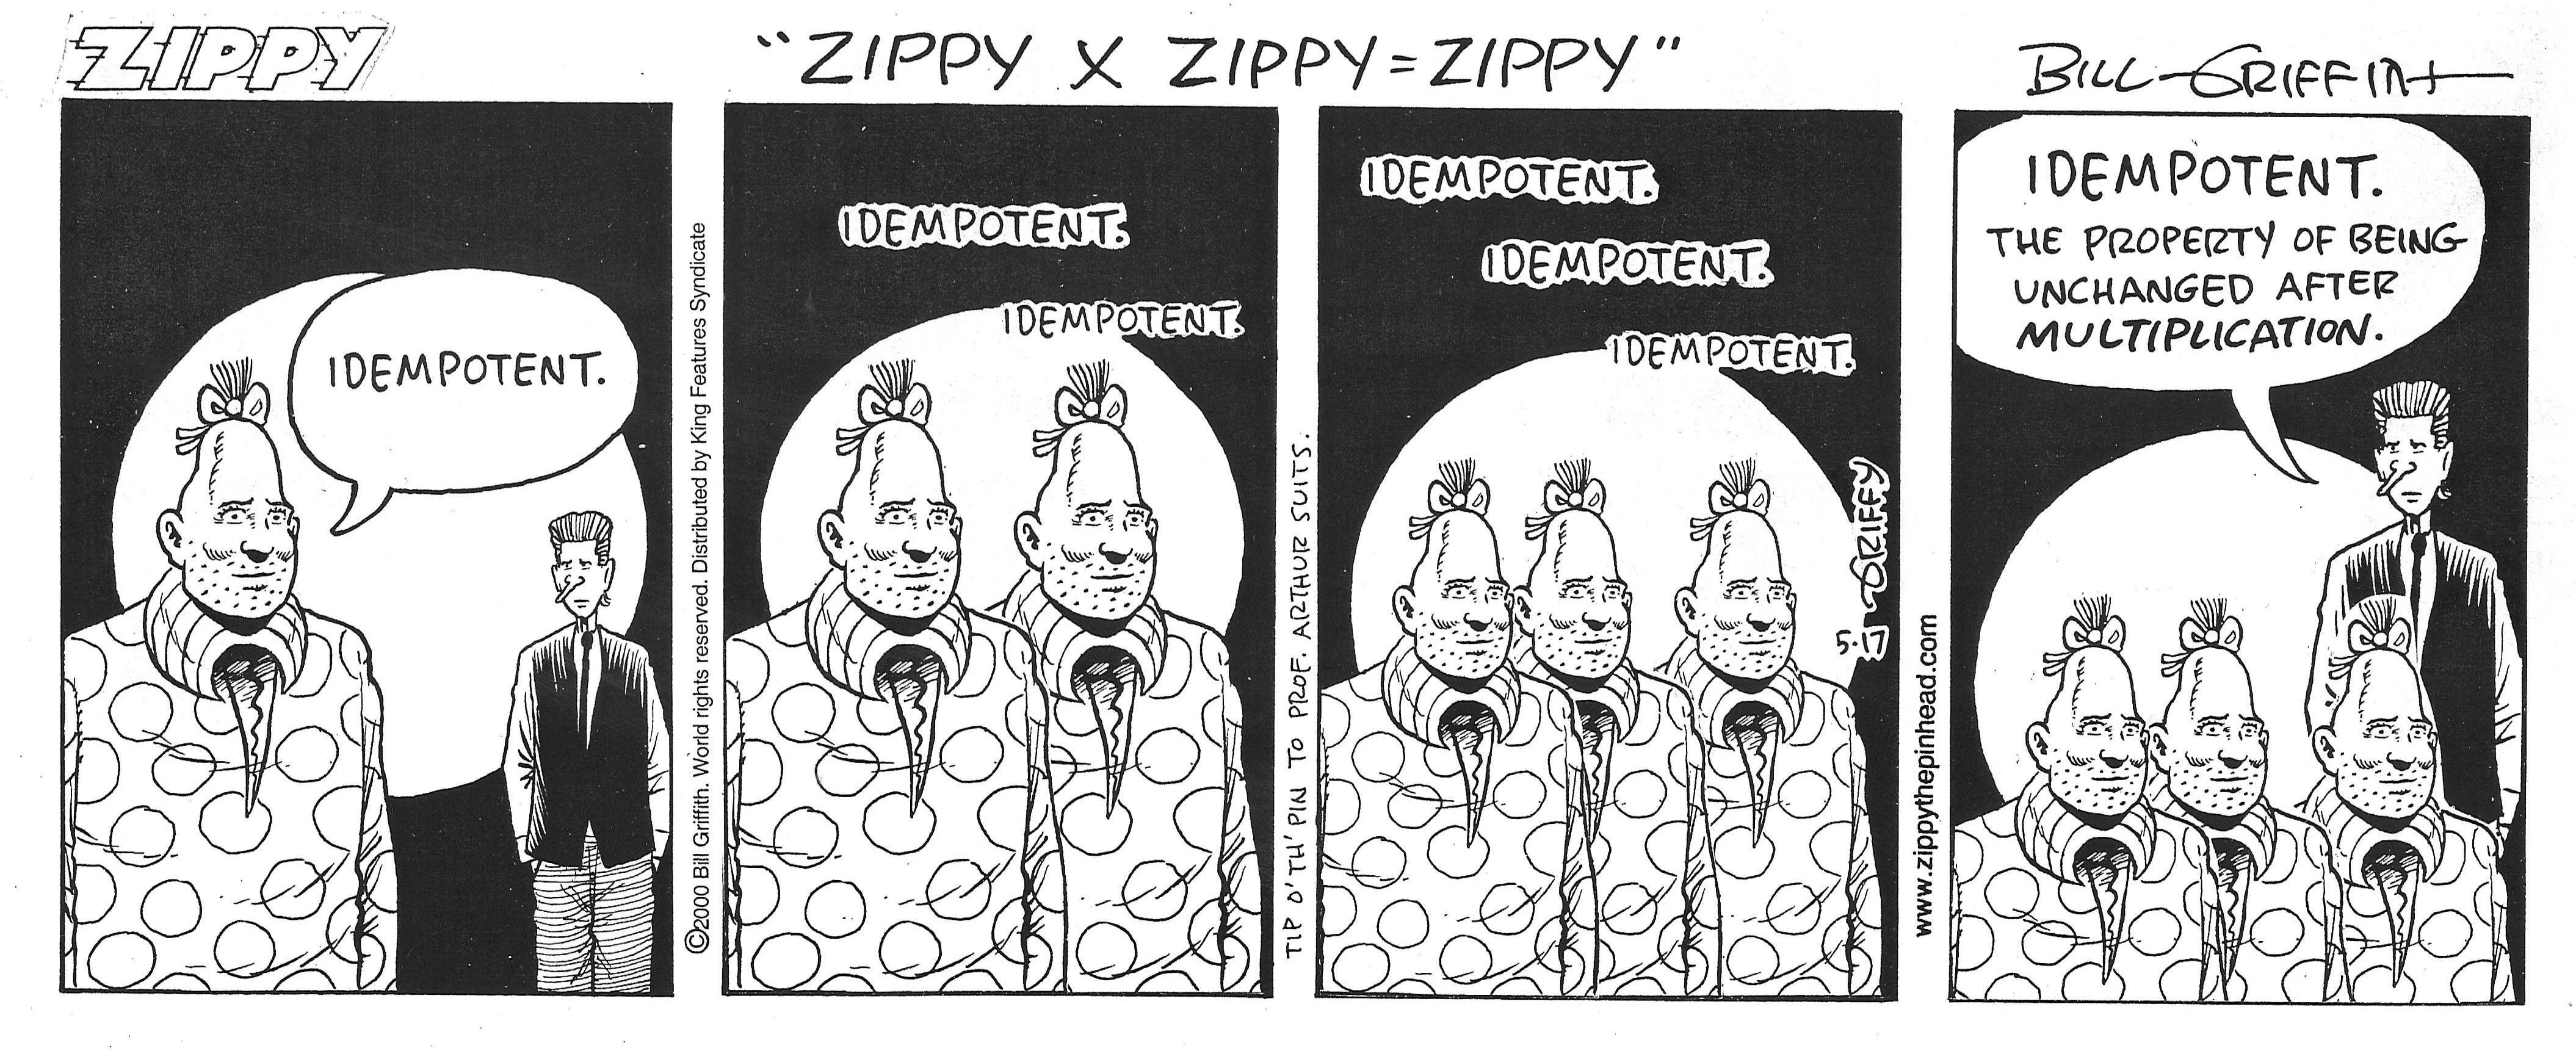
\includegraphics[width=1\linewidth]{zippy.png}
\caption{©  Bill Griffith. Reprinted with permission.\label{zip}}
\end{figure}
\par\smallskip
\end{exerciselist}
\typeout{************************************************}
\typeout{Section 2.3 The definition of a group}
\typeout{************************************************}
\section[{The definition of a group}]{The definition of a group}\label{section-5}
At this point you may be asking yourself, why do we care? We've covered a lot of definitions and proved some theorems, but what is the goal of all this? Well, there are actually many goals that we can achieve using such material. Consider the following as an example. Suppose we want to solve the equation \(5+x=2\). We can probably solve this quite easily almost just by looking at it (\(x=-3\)), but what facts are we actually using there? If we break down the reasoning leading to this answer, we may obtain something like the following, where each line is equivalent to the one preceding it.%
\begin{align*}
5+x\amp =2 \\
-5+(5+x)\amp =-5+2\\
(-5+5)+x \amp =-3\\
0+x\amp =-3\\
x\amp =-3.
\end{align*}
In the second line we add the inverse of \(5\) in \(\langle \Z, +\rangle\) to each side of the equation; in the third line we use associativity of \(+\) in \(\Z\) (along with computation); and in the fourth line we use the fact that \(-5\) is the additive inverse of \(5\) (that is, the inverse of \(5\) in \(\Z\) under \(+\)). Finally, we use the fact that 0 is an additive identity element in \(\Z\) (that is, the identity element in \(\Z\) under \(+\)).%
\par
In summary, we used \emph{associativity, identity elements, and inverses} in \(\Z\) to solve the given equation. This perhaps suggests that these would be useful traits for a binary structure and/or its operation to have. They are in fact so useful that a binary structure displaying these characteristics is given a special name. We note that these axioms are rather strong; ``most'' binary structures aren't groups.%
\begin{definition}[{}]\label{definition-19}
A \terminology{group} is a set \(G\), equipped with a binary operation \(*\), that satisfies the following three \terminology{group axioms}: \leavevmode%
\begin{enumerate}[label=\Roman*]
\item\hypertarget{li-74}{}\(*\) is associative on \(G\). (Axiom \(\G_1\))%
\item\hypertarget{li-75}{}There exists an identity element for \(*\) in \(G\). (Axiom \(\G_2\))%
\item\hypertarget{li-76}{}Every element \(a\in G\) has an inverse in \(G\). (Axiom \(\G_3\))%
\end{enumerate}
%
\par
We denote group \(G\) under \(*\) by the binary structure notation \(\langle G,*\rangle\), or simply by \(G\) if the operation \(*\) is known from context (or need not be known in the current situation).%
\end{definition}
\begin{remark}[]\label{remark-7}
When proving/disproving that a set \(G\) is/is not a group under an (apparent) operation \(*\): \leavevmode%
\begin{itemize}[label=\textbullet]
\item{}The first thing you should do is check to make sure that  \(\langle G,*\rangle\) is a binary structure by making sure \(G\) is closed under \(*\)\textemdash{}if not, it doesn't make sense to check to see if axioms \(\G_1\)\textendash{}\(\G_3\) hold). (For instance: \(\Z^*\) has no chance of being a group under \(\div\), since, e.g., \(3,4\in \Z^*\) but \(3 \div 4 \not\in\Z^*\).)%
\item{}You should never check \(\G_3\) before confirming \(\G_2\) holds, because it makes no sense to look for inverses if you haven't confirmed that \(G\) contains an identity element under \(*\).%
\end{itemize}
%
\end{remark}
\typeout{************************************************}
\typeout{Section 2.4 Examples of groups/nongroups, Part I}
\typeout{************************************************}
\section[{Examples of groups/nongroups, Part I}]{Examples of groups/nongroups, Part I}\label{section-6}
Let's look at some examples of groups/nongroups.%
\begin{example}[]\label{example-10}
We claim that \(\Z\) is a group under addition. Indeed, we already know that \(\Z\) is closed under addition and that addition is associative on the integers. The integer \(0\) acts as an identity element of \(\Z\) under addition (since \(a+0=0+a=a\) for each \(a\in
\Z\)), and each element \(a\) in \(G\) has inverse \(-a\) since \(a+(-a)=-a+a=0\).%
\end{example}
\begin{example}[]\label{example-11}
For each following binary structure \(\langle G,*\rangle\), determine whether or not \(G\) is a group. For those that are \emph{not} groups, determine the first group axiom  that fails, and provide a proof that it fails. \leavevmode%
\begin{multicols}{4}
\begin{enumerate}
\item\hypertarget{li-79}{}\(\langle \Q,+\rangle\)%
\item\hypertarget{li-80}{}\(\langle \Z,-\rangle\)%
\item\hypertarget{li-81}{}\(\langle \R,\cdot\rangle\)%
\item\hypertarget{li-82}{}\(\langle \C^*,\cdot\rangle\)%
\item\hypertarget{li-83}{}\(\langle \R,+\rangle\)%
\item\hypertarget{li-84}{}\(\langle \Z^+,+\rangle\)%
\item\hypertarget{li-85}{}\(\langle \Z^*,\cdot\rangle\)%
\item\hypertarget{li-86}{}\(\langle \M_n(\R),+\rangle\)%
\item\hypertarget{li-87}{}\(\langle \C,+\rangle\)%
\item\hypertarget{li-88}{}\(\langle \Z,\cdot\rangle\)%
\item\hypertarget{li-89}{}\(\langle \R^*,\cdot\rangle\)%
\item\hypertarget{li-90}{}\(\langle \M_n(\R),\cdot\rangle\)%
\end{enumerate}
\end{multicols}
%
\end{example}
If you have taken linear algebra, you have also probably seen a collection of matrices that is a group under matrix multiplication.%
\begin{definition}[{}]\label{definition-20}
\label{notation-32}
\label{notation-33}
Recall that given a square matrix \(A\), the notation \(\det A\) denotes the determinant of \(A\). Let%
\begin{equation*}
GL(n,\R)=\{M\in \M_n(\R):\det M \neq 0\}
\end{equation*}
(that is, let \(GL(n,\R)\) be  the set of all invertible \(n \times n\) matrices over \(\R\)) , and let%
\begin{equation*}
SL(n,\R)=\{M\in \M_n(\R):\det M =1\}\text{.}
\end{equation*}
These subsets of \(\M_n(\R)\) are called, respectively, the \terminology{general} and \terminology{special linear groups of degree \(n\) over \(\R\)}.%
\end{definition}
Note that these definitions imply that these subsets of \(\M_n(\R)\) are groups (under some operation). Sure enough, they are!%
\begin{theorem}[{}]\label{gl}
\label{notation-34}
 \(GL(n,\R)\) is a group under matrix multiplication.%
\end{theorem}
\begin{proof}\hypertarget{proof-7}{}
Let \(A,B\in GL(n, \R)\). Then \(\det(AB)=(\det A)(\det B) \neq 0\) (since \(\det A, \det B \neq 0)\), so \(AB\in GL(n,\R)\).  Thus, \(\langle GL(n,\R), \cdot\rangle\) is a binary structure.%
\par
We know that matrix multiplication is always associative,so \(\G_2\) holds. Next,%
\begin{equation*}
I_n= \begin{bmatrix}1 \amp  0 \amp  0 \amp  \cdots \amp  0 \\
0 \amp  1 \amp  0 \amp  \cdots \amp  0 \\
0 \amp  0 \amp  1 \amp  \cdots \amp  0 \\
\vdots \amp  \vdots \amp  \vdots \amp  \ddots \amp  \vdots \\
0 \amp  0 \amp  0 \amp  \cdots \amp  1
\end{bmatrix},
\end{equation*}
the  is in \(GL(n,\R)\)since \(\det I_n=1\neq 0\), and it acts as an identity element for \(\langle GL(n,\R), \cdot\,\rangle\) since%
\begin{equation*}
AI_n=I_nA = A
\end{equation*}
for all \(A\in GL(n,\R)\).%
\par
Finally, let \(A\in GL(n,\R)\).  Since \(\det A\neq 0\), \(A\) has (matrix multiplicative) inverse \(A^{-1}\) in \(\M_2(\R)\). But we need to verify that \(A^{-1}\) is in \(G\). This is in fact the case, however, since \(A^{-1}\) is invertible (it has inverse \(A\)), hence \(\det
A^{-1} \neq 0\).  Thus, \(A^{-1}\) is also in \(GL(n,\R)\).%
\par
So \(GL(n,\R)\) is a group under multiplication.%
\end{proof}
\begin{theorem}[{}]\label{sl}
\(SL(n,\R)\), is a group under matrix multiplication.%
\end{theorem}
\begin{proof}\hypertarget{proof-8}{}
Let \(A,B\in SL(n, \R)\). Then \(\det(AB)=(\det A)(\det B) =1(1)=1\), so \(AB\in SL(n,\R)\).  Thus, \(\langle SL(n,\R), \cdot\rangle\) is a binary structure.%
\par
The rest of the proof is left as an exercise for the reader.%
\end{proof}
\begin{remark}[]\label{remark-8}
Throughout this course, if we are discussing a set \(GL(n,\R)\) or \(SL(n,\R)\), you should assume \(n\in \Z^+\), unless otherwise noted.%
\end{remark}
We end this section with a final example.%
\begin{example}[]\label{example-12}
Define \(*\) on \(\Q^*\) by \(a*b=(ab)/2\) for all \(a,b\in \Q^*\). Prove that \(\langle \Q^*,*\rangle\) is a group.%
\par\medskip\noindent%
\textbf{Solution.}\quad First, \(\Q^*\) is closed under \(*\), since \((ab)/2\) is rational and nonzero whenever \(a,b\) are rational and nonzero.%
\par
Next, we check that \(\Q^*\) under \(*\) satisfies the group axioms. Since multiplication is commutative on \(\Q\), \(*\) is clearly commutative on \(\Q^*\), and so our work to show \(\G_2\) and \(\G_3\) is marginally reduced.%
\par
First, associativity of \(*\) on \(\Q^*\) is inherited from associativity of multiplication on \(\Q^*\).%
\par
Notice that the perhaps ``obvious'' choice, 1, is \emph{not} an identity element for \(\Q^*\) under \(*\): for instance, \(1*3=3/2 \neq 3\). Rather, \(e\) is such an identity element if and only if for all \(a\in \Q\) we have \(a=e*a=(ea)/2\). We clearly have \(a=(2a)/2\) for all \(a\in \Q^*\); so \(2\) acts as an identity element for \(\Q^*\) under \(*\).%
\par
Finally, let \(a\in \Q^*\).  Since \(a\neq 0\), it makes sense to divide by \(a\); then \(4/a\in \Q^*\), with \(a*(4/a)=(a(4/a))/2=2\).%
\par
Thus, \(\langle \Q^*,*\rangle\) is a group.%
\end{example}
\typeout{************************************************}
\typeout{Section 2.5 Group conventions and properties}
\typeout{************************************************}
\section[{Group conventions and properties}]{Group conventions and properties}\label{section-7}
Before we discuss more examples, we present a theorem and look at some conventions we follow and notation we use when discussing groups in general; we also discuss some properties of groups.%
\typeout{************************************************}
\typeout{Subsection 2.5.1 Some group conventions}
\typeout{************************************************}
\subsection[{Some group conventions}]{Some group conventions}\label{subsection-1}
\begin{theorem}[{}]\label{theorem-9}
The identity element of a group is unique (by \hyperref[uniqueid]{Theorem~\ref{uniqueid}}), and given any element \(a\) of a group \(G\), the inverse of \(a\) in \(G\) is unique (by \hyperref[uniqueinverse]{Theorem~\ref{uniqueinverse}}).%
\end{theorem}
\begin{observation}[]\label{observation-1}
\label{notation-35}
 \label{notation-36}
We will generally use \(e\) or \(e_G\) as our default notation for an identity element of group, but be aware that many mathematicians denote a group's identity element by 1. We  denote the inverse of element \(a\) in \(G\) by \(a^{-1}\).%
\end{observation}
\begin{warning}[]\label{warning-6}
Although it is written in what we call  \emph{multiplicative notation}, do \emph{not} assume \(a^{-1}\) is what we usually think of as a multiplicative inverse for \(a\); remember, we don't even know if elements of a group are numbers! The type of inverse that \(a^{-1}\) is (a multiplicative inverse for a real number? an additive inverse for a real number? a multiplicative inverse for a matrix? an inverse function for a function from \(\R\) to \(\R\)?) depends on both \(G\)'s elements and its operation.%
\end{warning}
\begin{convention}[]\label{convention-1}
\leavevmode%
\begin{itemize}[label=\textbullet]
\item{}We usually \emph{don't} use the notation \(*\) when describing group operations. Instead, we use the multiplication symbol \(\cdot\) for the operation in an arbitrary group, and  call applying the operation ``multiplying''\textemdash{}even though the operation may not be ``multiplication'' in the non-abstract, traditional sense! It may actually be addition of real numbers, composition of functions, etc. Moreover, when actually operating in a group \(\langle G, \cdot\,\rangle\), we typically omit the \(\cdot\) . That is, for \(a,b\in G\), we write the product \(a\cdot b\) as \(ab\). We call this the ``product'' of \(a\) and \(b\).%
\par
For every element \(a\) in a group \(\Gdot\) and \(n\in \Z^+\), we use the expression \(a^n\) to denote  the product%
\begin{equation*}
a \times a \times \cdots \times a
\end{equation*}
of \(n\) copies of \(a\), and \(a^{-n}\) to denote \((a^{-1})^n\) (that is, the product of \(n\) copies of \(a^{-1}\)). Finally, we define \(a^0\) to be \(e\).  Note that our ``usual'' rules for exponents then hold in an arbitrary group: that is, if \(a\) is in group \(\langle G, \cdot\,\rangle\) and \(m,n\in \Z\), then \(a^m a^n = a^{m+n}\) and \((a^m)^n=a^{mn}=(a^n)^m\).%
\par
However:%
\item{}\label{notation-37}
 When we know our operation is commutative, we typically use additive notation, denoting the group operation by \(+\), calling the group operation ``addition,'' and denoting the inverse of an element \(a\) by \(-a\). When we use additive notation, we do \emph{not} omit the \(+\) when operating in a group \(\langle G,+\rangle\), and we call \(a+b\) a \emph{sum} rather than a product. Also, when working with an operation that is known to be commutative,  the identity element may be denoted by 0 rather than by \(e\), \(e_G\), or 1, and for \(n\in \N\), we write \(na\) instead of \(a^n\).%
\par
Finally, note that \((-n)a=n(-a)=-(na)\) (where \(-a\) and \(-(na)\) indicate the additive inverses of \(a\) and \(na\), respectively); we can therefore unambiguously use the notation \(-na\) for this element. Using this notation, note that for \(m\in \Z\), \(na+ma=(n+m)a\) and \(n(ma)=(nm)a\).%
\end{itemize}
%
\end{convention}
\begin{warning}[]\label{warning-7}
Be careful to always know where an element you are working with lives! For instance, if, as above, \(n\in
\Z^+\) and \(a\) is a group element, \(-n\) and \(-a\) look similar but may mean very different things. While \(-n\) is a negative integer, \(-a\) may be the additive inverse of a matrix in \(\M_2(\R)\), the additive inverse 2 of the number 4 in \(\Z_6\), or even something completely unrelated to numbers.%
\end{warning}
\begin{remark}[]\label{remark-9}
Multiplicative notation can be used when working with any arbitary group, while additive notation should be used only when working with a group whose binary operation is commutative.%
\end{remark}
We summarize multiplicative versus addition notation in the following table, where \(a,b\) are elements of a group \(G\).%
\begin{table}
\centering
\begin{tabular}{lll}
\multicolumn{1}{c}{}&\multicolumn{1}{c}{Multiplicative notation}&\multicolumn{1}{c}{Additive notation}\tabularnewline\hrulemedium
Operation notation&\multicolumn{1}{c}{\(\cdot\)}&\multicolumn{1}{c}{\(+\)}\tabularnewline[0pt]
\(a\) operated with \(b\)&\multicolumn{1}{c}{\(ab\)}&\multicolumn{1}{c}{\(a+b\)}\tabularnewline[0pt]
Identity element&\multicolumn{1}{c}{\(e\) or \(e_G\) (or \(1\))}&\multicolumn{1}{c}{\(e\) or \(e_G\) (or \(0\))}\tabularnewline[0pt]
Inverse of \(a\)&\multicolumn{1}{c}{\(a^{-1}\)}&\multicolumn{1}{c}{\(-a\)}
\end{tabular}
\caption{Summary of multiplicative and addition notation in groups.\label{table-1}}
\end{table}
\begin{convention}[]\label{convention-2}
We \emph{do} use the notation \(*\) when using multiplicative or additive notation would lead to confusion. For instance, if we want to define an operation on \(\Q^*\) that assigns to pair \((a,b)\) the quantity \(ab/2\), it would be unwise to use multiplicative or additive notation for this operation since we already have conventional meanings of \(ab\) and \(a+b\). Similarly, we would not denote the identity element of \(\Q^*\) under this operation by \(0\) or \(1\), since the identity element in this group is the rational number \(2\), and writing \(0=2\) or \(1=2\) would look weird.%
\end{convention}
Finally:%
\begin{convention}[]\label{convention-3}
If there is a default notation for a particular operation (say, \(\circ\) for composition of functions) or identity element (say, \(I_n\) in \(GL(n,\R)\)) we usually use that notation instead.%
\end{convention}
\typeout{************************************************}
\typeout{Subsection 2.5.2 Some group properties}
\typeout{************************************************}
\subsection[{Some group properties}]{Some group properties}\label{subsection-2}
While we don't need to worry about ``order'' when multiplying a group element \(a\) by itself, we \emph{do} need to worry about it in general.%
\begin{warning}[]\label{warning-8}
Group operations need \emph{not} be commutative!%
\end{warning}
\begin{definition}[{}]\label{definition-21}
A group \(\langle G, \cdot\,\rangle\) is said to be \terminology{abelian} if \(ab=ba\) for all \(a,b\in
G\). Otherwise, \(G\) is \terminology{nonabelian}. (The word ``abelian'' derives from the surname of mathematician Niels Henrik Abel.)%
\end{definition}
\begin{remark}[]\label{remark-10}
If we know that a binary operation \(\cdot\) on a set \(G\) is commutative, then in checking to see if axioms \(\G_2\) and \(\G_3\) hold we need only verify that there exists \(e\in G\) such that \(ae=a\) (we don't need to check that \(ea=a\)) for all \(a\in G\) and that for each \(a\in G\) there exists \(b\in G\) such that \(ab=e\) (we don't need to check that \(ba=e\)).%
\end{remark}
\begin{remark}[]\label{remark-11}
If \(G\) is not known to be abelian, we must be careful when multiplying elements of \(G\) by one another: multiplying on the left is, in general, not the same as multiplying on the right!%
\end{remark}
\begin{definition}[{}]\label{definition-22}
If \(G\) is a group, then the cardinality \(|G|\) of \(G\) is called the \terminology{order of \(G\)}. If \(|G|\) is finite, then \(G\) is said to be a \terminology{finite group}; otherwise, it's an \terminology{infinite group}.%
\end{definition}
\begin{example}[]\label{example-13}
Of the groups we've discussed, which are abelian? Which are infinite/finite?%
\end{example}
We have already seen that identity elements of groups are unique, and that each element \(a\) of a group \(G\) has a unique inverse \(a^{-1}\in G\). Here are some other basic properties of groups.%
\begin{theorem}[{}]\label{cancel}
If \(\Gdot\) is a group, then \emph{\emph{left and right cancellation laws}} hold in \(G\). That is, if \(a,b,c\in G\), then \leavevmode%
\begin{enumerate}
\item\hypertarget{li-93}{}If \(ab=ac\), we have \(b=c\) (the left cancellation law); and%
\item\hypertarget{li-94}{}If \(ba=ca\), we have \(b=c\) (the right cancellation law).%
\end{enumerate}
%
\end{theorem}
\begin{proof}\hypertarget{proof-9}{}
Let \(a,b,c\in G\) and assume that \(ab=ac\). Multiplying both equation sides on the left by \(a^{-1}\), we obtain%
\begin{align*}
{2}
\amp \amp  a^{-1}(ab)\amp =a^{-1}(ac)\\
\amp \Rightarrow
\amp (a^{-1}a)b\amp =(a^{-1}a)c\\
\amp \Rightarrow
\amp eb\amp =ec\\
\amp \Rightarrow
\amp b\amp =c
\end{align*}
%
\par
This proves that the left cancellation law holds. A similar proof shows that the right cancellation law holds.%
\end{proof}
\begin{theorem}[{}]\label{uniquesols}
Let \(\Gdot\) be a group and let \(a,b\in G\). Then there exist \emph{\emph{unique}} elements \(x,y\in G\) such that \(ax=b\) and \(ya=b\).%
\end{theorem}
\begin{proof}\hypertarget{proof-10}{}
If \(x=a^{-1}b\) and \(y=ba^{-1}\), then \(ax=a(a^{-1}b)=(aa^{-1})b=eb=b\) and \(ya=(ba^{-1})a=b(a^{-1}a)=be=b\). So such elements \(x\) and \(y\) exist. The fact that they are unique follows from the cancellation laws: if \(ax=b\) and \(ax'=b\) then \(x=x'\) by left cancellation, and if \(ya=b\) and \(y'a=b\) then \(y=y'\) by right cancellation.%
\end{proof}
\begin{warning}[]\label{warning-9}
We only of necessity have \((ab)^{-1}=a^{-1}b^{-1}\) if \(G\) is known to be abelian!%
\end{warning}
However, we do have the following:%
\begin{theorem}[{}]\label{invofprod}
If \(a\) and \(b\) are elements of a group \(\Gdot\), then%
\begin{equation*}
(ab)^{-1}=b^{-1}a^{-1}.
\end{equation*}
%
\end{theorem}
\begin{proof}\hypertarget{proof-11}{}
We have that%
\begin{equation*}
(ab)(b^{-1}a^{-1})=a(bb^{-1})a^{-1}=aea^{-1}=aa^{-1}=e.
\end{equation*}
%
\par
Similarly, \((b^{-1}a^{-1})(ab)=e\).%
\end{proof}
\typeout{************************************************}
\typeout{Section 2.6 Examples of groups/nongroups, Part II}
\typeout{************************************************}
\section[{Examples of groups/nongroups, Part II}]{Examples of groups/nongroups, Part II}\label{section-8}
\begin{example}[]\label{example-14}
\label{notation-38}
 Let \(n\in \Z^+\). We define \(n\Z\) by%
\begin{equation*}
n\Z=\{nx: x\in \Z\}:
\end{equation*}
that is, \(n\Z\) is the set of all (integer) multiples of \(n\).%
\end{example}
\begin{theorem}[{}]\label{nz}
\(n\Z\) is a group under \(+\) (the usual addition of integers).%
\end{theorem}
\begin{proof}\hypertarget{proof-12}{}
Let \(x, y\in n\Z\). Then there exist \(a,b\in \Z\) such that \(x=na\) and \(y=nb\). Then \(x+y=na+nb=n(a+b)\in n\Z\). So \(\langle n\Z,+\rangle\) is a binary structure. The remainder of the proof is left as an exercise for the reader.%
\end{proof}
\begin{remark}[]\label{remark-12}
When we are discussing a group \(n\Z\), assume that \(n\in \Z^+\), unless otherwise noted.%
\end{remark}
We use an example from our next class of groups all the time; in fact, most six-year-olds do as well, since it is used when telling time! Before we get to the example, we need some more definitions and some notation. Throughout the following discussion, assume \(n\) is a fixed positive integer.%
\begin{definition}[{}]\label{definition-23}
\label{notation-39}
We say integers \(a\) and \(b\) are \terminology{congruent modulo [or mod] \(n\)} if \(n\) divides \(a-b\). If \(a\) and \(b\) are congruent mod \(n\), we write \(a \equiv_n b\).%
\end{definition}
\begin{example}[]\label{cong_ex}
\(1, 7, 13,\) and \(-5\) are all congruent mod \(6\).%
\end{example}
The following is a profoundly useful theorem; it's so important, it has a special name. We omit the proof of this theorem, but direct interested readers to for, instance, p. 5 in~\hyperlink{NZM}{[3]}.%
\begin{theorem}[{Division Algorithm}]\label{divalg}
Let \(n\in \Z^+\) and let \(a\) be any integer. Then there exist unique integers \(q\) and \(r\), with \(0\leq
r \lt n\), such that \(a=qn+r\).%
\par
(This is actually a special case of a more general theorem, which states that given any integers \(n\) and \(a\), there exist unique integers \(q\) and \(r\), with \(0\leq
r\lt |n|\), such that \(a=qn+r\).)%
\end{theorem}
It follows that for each positive integer \(n\) and integer \(a\), there exists a unique element \(R_n(a)\) (the \(r\) in the above theorem) of the set \(\{0,1,2,\ldots, n-1\}\) such that \(a\) is congruent to \(R_n(a)\) modulo \(n\). For example, \(R_3(4)=1\), \(R_3(0)=0\), \(R_3(17)=2\), and \(R_3(-5)=1\).%
\begin{definition}[{}]\label{definition-24}
\label{notation-40}
\(R_n(a)\) is the \terminology{remainder} when we divide \(a\) by \(n\). (Note: You were probably already familiar with the remainder when you divide a positive integer by \(n\).)%
\end{definition}
\begin{definition}[{}]\label{definition-25}
\label{notation-41}
We define \terminology{addition modulo \(n\)}, \(+_n\), on \(\Z\) by, for all \(a,b\in \Z\),%
\begin{equation*}
a+_n b=R_n(a+b),
\end{equation*}
that is, the unique element of \(\{0,1,\ldots, n-1\}\) that's congruent to the integer \(a+b\) modulo \(n\).%
\end{definition}
\begin{remark}[]\label{remark-13}
Addition mod 24 is what we use to tell time!%
\end{remark}
The set \(\{0,1,2,\ldots, n-1\}\) of remainders when dividing by \(n\) is so important we give it a special notation.%
\begin{definition}[{}]\label{definition-26}
We define \(\Z_n\) to be the set \(\{0,1,2,\ldots,n-1\}\).%
\end{definition}
Throughout this course, if we are discussing a set \(\Z_n\), you should assume \(n\in \Z^+, n\geq 2\), unless otherwise noted. (Though it will rarely come up for us, we may occasionally make reference to \(\Z_1=\{0\}\).)%
\begin{warning}[]\label{warning-10}
Note that by our definition of \(\Z_n\), the integer \(n\) itself is \emph{not} in \(\Z_n\)!%
\end{warning}
We are now ready to consider our next type of group.%
\begin{example}[]\label{example-16}
\label{notation-42}
 For each \(n\in \Z^+\), \(\langle \Z_n,+_n\rangle\) is a group, called the \emph{cyclic group of order \(n\)} (we will see later why we use the word ``cyclic'' here). This group is abelian and of order \(n\).%
\par\medskip\noindent%
\textbf{Solution.}\quad We first check that \(\Z_n\) is closed under \(+_n\). Note that by the definition of \(+_n\), \(a+_nb \in \Z_n\) for each \(a,b\in \Z\). Thus, \(a+_nb \in \Z_n\) for each \(a,b\in \Z_n\).%
\par
We next check that \(\Z_n\) under \(+_n\) satisfies the three group axioms. Note that since addition is commutative on \(\Z\),%
\begin{equation*}
a+_n b =R_n(a+b)=R_n(b+a)=b+_n a
\end{equation*}
for all \(a,b\in \Z_n\). Again, a simpler way of stating this is that commutativity of \(+_n\) on \(\Z_n\) is inherited from the commutativity of addition on \(\Z\). One nice result of this is that since \(+_n\) is commutative on \(\Z_n\), we have less to check when verifying group axioms \(\G_2\) and \(\G_3\).%
\par
Now, let \(a,b,c\in \Z_n\).  We want to show that \((a+_n b)+_n c = a +_n(b+_n c)\). Now,%
\begin{align*}
(a+_n b)+_n c\amp =R_n(a+b)+_n c\\
\amp \equiv_n R_n(a+b)+c\\\
\amp \equiv_n (a+b)+c\\\
\amp \equiv_n a+(b+c)\\
\amp \equiv_n a+R_n(b+c)\\
\amp \equiv_n a+_n (b+_n c).
\end{align*}
So \((a+_n b)+_n c\) and \(a+_n (b+_n c)\) are congruent mod \(n\).  Since both of these values are in \(\{0,1,\ldots, n-1\}\), this implies that they are equal, as desired.%
\par
Next, clearly, \(0\in \Z_n\) acts as an identity element under \(+_n\), since%
\begin{equation*}
0+_n a =R_n(0+a)=R_n(a)
\end{equation*}
for each \(a\in \Z_n\).%
\par
Finally, let \(a\in \Z_n\).  If \(a=0\), then clearly \(a\) has inverse \(0\in \Z_n\) since \(0+_n 0 = 0\). If \(a\neq 0\), then the element \(n-a\in \Z_n\) is an inverse for \(a\) since%
\begin{equation*}
a+_n(n-a)=R_n(a+(n-a))=R_n(n)=0.
\end{equation*}
%
\par
Since \(+_n\) is commutative on \(\Z_n\), \(\Z_n\) is an abelian group under \(+_n\).%
\par
Finally, we already know that \(|\Z_n|=|\{0,1,2,\ldots,n-1\}|=n\).%
\end{example}
\begin{remark}[]\label{remark-14}
In practice, we often omit the subscript \(n\) and just write \(+\) when discussing addition modulo \(n\) on \(\Z_n\).%
\end{remark}
\begin{warning}[]\label{warning-11}
Do not confuse \(n\Z\) and \(\Z_n\)! They are very different as sets and as groups.%
\end{warning}
\begin{example}[]\label{example-17}
In the group \(\langle \Z_8,+\rangle\) (where, as indicated by our above remark, \(+\) means addition modulo \(8\)), we have, for instance, \(3+7=2\) and \(7+7=6\). The numbers 2 and 6 are each other's inverse, and \(7^{-1}=1\). The number \(0\) has inverse \(0\) (it can't be \(8\), since \(8\not\in \Z_8\)!).%
\end{example}
\begin{definition}[{}]\label{definition-27}
For \(n\in \Z^+\), we define \terminology{multiplication modulo \(n\)}, denoted \(\cdot_n\), on \(\Z_n\) by \(a\cdot_n b = r_n(a)\), the remainder when \(ab\) is divided by \(n\).%
\end{definition}
\begin{remark}[]\label{remark-15}
\(\Z_n\) is never a group under \(\cdot_n\) (do you see why?).%
\end{remark}
But we can consider the following%
\begin{definition}[{}]\label{definition-28}
\label{notation-43}
For \(n\in \Z^+\), we define \(\Z_n^{\times}\) to be the set%
\begin{equation*}
\{a\in \Z_n\,:\,\gcd(a,n)=1\}\text{.}
\end{equation*}
%
\end{definition}
\begin{example}[]\label{example-18}
\(\langle \Z_n^{\times},\,\cdot\, \rangle\) is a group under multiplication. We omit the proof.%
\end{example}
We end this section by considering a few more examples.%
\begin{example}[]\label{funcrr}
\label{notation-44}
 Let \(F\) be the set of all functions from \(\R\) to \(\R\), and define \emph{pointwise addition} \(+\) on \(F\) by%
\begin{equation*}
(f+g)(x)=f(x)+g(x)
\end{equation*}
for all \(f,g\in F\) and \(x\in \R\). We claim that \(F\) is a group under pointwise addition. (For variety, in this proof we don't explicitly refer to \(\G_1\)\textendash{}\(\G_3\), though we certainly do verify they hold.) Indeed, if \(f,g\in F\) then clearly \(f+g\) is also a function from \(\R\) to \(\R\), so \(F\) is closed under \(+\).%
\par
Next, let \(f,g,h\in F\). Then for all \(x\in \R\),%
\begin{align*}
((f+g)+h)(x)\amp =(f+g)(x)+h(x)\amp \amp\\
\amp =((f(x)+g(x))+h(x)\amp \amp\\
\amp =f(x)+(g(x)+h(x))\amp \amp \text{ (since addition is associative on
\(\R\)) }\\
\amp =f(x)+(g+h)(x)\amp \amp\\
\amp =(f+(g+h))(x)\amp \amp .
\end{align*}
%
\par
Note that the key fact used in this argument is that \(f(x)\), \(g(x)\) and \(h(x)\) all lie in \(\R\), and addition is associative on \(\R\). When you get used to such arguments, it is sufficient to say that associativity of \(+\) on \(F\) is \emph{inherited} from the associativity of addition on \(\R\).%
\par
Next, let \(z:\R\to\R\) be the function \(z(x)=0\) for all \(x\). Then for all \(f\in F\) and \(x\in \R\),%
\begin{align*}
(f+z)(x)\amp =f(x)+z(x)\amp \amp\\
\amp =f(x)+0\amp \amp\\
\amp =f(x)\amp \amp \\
\amp =0+f(x)\amp \amp\\
\amp =z(x)+f(x)\amp \amp\\
\amp = (z+f)(x).
\end{align*}
%
\par
So \(z\) is an identity element of \(\langle F,+\rangle\).%
\par
Finally, let \(f\in F\), and define \(g\in F\) by \(g(x)=-f(x)\) for all \(x\in \R\). It is easy then to see that \(g\) is an inverse for \(f\) in \(F\).%
\par
Hence, \(F\) is a group under pointwise addition. Note that it is uncountably infinite and abelian.%
\end{example}
\begin{example}[]\label{bijrr}
\label{notation-45}
 The set \(F\) is \emph{not} a group under function composition (do you see why?). But if we define \(B\) to be the set of all \emph{bijections} from \(\R\) to \(\R\), then \(B\) is a group under function composition. (Prove it!) \(B\) is uncountably infinite and nonabelian.%
\end{example}
\begin{example}[]\label{gpprod}
Let \(\langle G_1,*_1\rangle\), \(\langle G_2,*_2\rangle\) , \(\ldots\), \(\langle G_n,*_n\rangle\) be groups (\(n\in \Z^+\)). Then the \emph{group product}%
\begin{equation*}
G=G_1\times G_2\times \cdots \times G_n
\end{equation*}
is a group under the \emph{componentwise} operation \(*\) defined by%
\begin{equation*}
(g_1,g_2,\ldots, g_n)*(h_1,h_2,\ldots,h_n)=(g_1*_1h_1, g_2*_2h_2,\ldots, g_n*_nh_n)
\end{equation*}
for all \((g_1,g_2,\ldots, g_n),(h_1,h_2,\ldots,h_n)\in G\).%
\par
For instance, considering multiplication on \(\R^*\), matrix multiplication on \(GL(2,\R)\), and addition modulo \(6\) on \(\Z_6\), we have that \(\langle \R^*\times GL(2,\R) \times \Z_6,*\rangle\) is a group in which, for instance,%
\begin{equation*}
\left(-1, \begin{bmatrix}
1 \amp  \phantom{-}3 \\
0 \amp  -1
\end{bmatrix},
3\right)
*\left(\pi,
\begin{bmatrix}
2 \amp  1 \\
1 \amp  1
\end{bmatrix},
4\right)=\left(-\pi,
\begin{bmatrix}
\phantom{-}5 \amp  \phantom{-}4 \\
-1 \amp -1
\end{bmatrix}
,1\right).
\end{equation*}
%
\end{example}
\begin{example}[]\label{example-22}
A common example of a group product is the group \(\Z_2^2\), equipped with componentwise addition modulo 2.%
\end{example}
\begin{definition}[{}]\label{definition-29}
The group \(\Z_2^2\) is known as the \terminology{Klein 4-group}. (Felix Klein was a German mathematician; you may have heard of him in relation to the Klein Bottle.) The group \(\Z_2^2\) is sometimes denoted by \(V\), which stands for ``Vierergruppe,'' the German word for ``four-group''.%
\end{definition}
\typeout{************************************************}
\typeout{Section 2.7 Summaries of groups we've seen}
\typeout{************************************************}
\section[{Summaries of groups we've seen}]{Summaries of groups we've seen}\label{section-9}
When you see the following groups in the wild, you should assume they are equipped with the following default operations, unless otherwise noted.  You should know: \leavevmode%
\begin{itemize}[label=\textbullet]
\item{}What elements the groups contain;%
\item{}What their default operations are;%
\item{}Their orders (and, if they're infinite, whether they're countably infinite or uncountable);%
\item{}Whether or not they are abelian.%
\end{itemize}
%
% group protects changes to lengths, releases boxes (?)
{% begin: group for a single side-by-side
% set panel max height to practical minimum, created in preamble
\setlength{\panelmax}{0pt}
\newsavebox{\panelboxEtabular}
\savebox{\panelboxEtabular}{%
\raisebox{\depth}{\parbox{1\linewidth}{\centering\begin{tabular}{ll}
\emph{Group(s)}&\emph{Operation}\tabularnewline\hrulemedium
\(\Z\), \(\Q\)&addition of numbers\tabularnewline[0pt]
\(n\Z\)&addition of numbers\tabularnewline[0pt]
\(\R\), \(\C\)&addition of numbers\tabularnewline[0pt]
\(\Q^*\), \(\Q^+\)&multiplication of  numbers\tabularnewline[0pt]
\(\R^*\), \(\R^+\), \(\C^*\)&multiplication of  numbers\tabularnewline[0pt]
\(\M_{m\times n}(\R), \M_n(\R)\)&matrix addition\tabularnewline[0pt]
\(GL(n,\R), SL(n,\R)\)&matrix multiplication\tabularnewline[0pt]
\(\Z_n\)&addition mod \(n\)\tabularnewline[0pt]
\(\Z_2^2\)&componentwise addition mod 2\tabularnewline[0pt]
\(F\)  (see \hyperref[funcrr]{Example~\ref{funcrr}})&pointwise addition\tabularnewline[0pt]
\(B\) (see \hyperref[bijrr]{Example~\ref{bijrr}})&composition
\end{tabular}
}}}
\newlength{\phEtabular}\setlength{\phEtabular}{\ht\panelboxEtabular+\dp\panelboxEtabular}
\settototalheight{\phEtabular}{\usebox{\panelboxEtabular}}
\setlength{\panelmax}{\maxof{\panelmax}{\phEtabular}}
\leavevmode%
% begin: side-by-side as tabular
% \tabcolsep change local to group
\setlength{\tabcolsep}{0\linewidth}
% @{} suppress \tabcolsep at extremes, so margins behave as intended
\par\medskip\noindent
\begin{tabular}{@{}*{1}{c}@{}}
\begin{minipage}[c][\panelmax][t]{1\linewidth}\usebox{\panelboxEtabular}\end{minipage}\end{tabular}\\
% end: side-by-side as tabular
}% end: group for a single side-by-side
\typeout{************************************************}
\typeout{Exercises 2.8 Exercises, Part II}
\typeout{************************************************}
\section[{Exercises, Part II}]{Exercises, Part II}\label{exercises-3}
\begin{exerciselist}
\item[1.]\hypertarget{exercise-12}{}True/False. For each of the following, write T if the statement is true; otherwise, write F. You do NOT need to provide explanations or show work for this problem. \leavevmode%
\begin{enumerate}[label=(\alph*)]
\item\hypertarget{li-99}{}For every positive integer \(n\), there exists a group of order \(n\).%
\item\hypertarget{li-100}{}For every integer \(n\geq 2\), \(\Z_n\) is abelian.%
\item\hypertarget{li-101}{}Every abelian group is finite.%
\item\hypertarget{li-102}{}For every integer \(m\) and integer \(n>2\), there exist infinitely many integers \(a\) such that \(a\) is congruent to \(m\) modulo \(n\).%
\item\hypertarget{li-103}{}A binary operation \(*\) on a set \(S\) is commutative if and only if there exist \(a,b\in S\) such that \(a*b=b*a\).%
\item\hypertarget{li-104}{}If \(\langle S, *\rangle\) is a binary structure, then the elements of \(S\) must be numbers.%
\item\hypertarget{li-105}{}If \(e\in \langle S,*\rangle\) is an identity element of \(S\), then \(e\) is an idempotent in \(S\) (that is, \(e*e=e\)).%
\item\hypertarget{li-106}{}If \(s\in \langle S,*\rangle\) is an idempotent, then \(s\) must be an identity element of \(S\).%
\end{enumerate}
%
\par\smallskip
\item[2.]\hypertarget{exercise-13}{}Let \(G\) be the set of all functions from \(\Z\) to \(\R\). Prove that pointwise multiplication on \(G\) is commutative. (\emph{Note.} To prove that two functions, \(h\) and \(j\), sharing the same domain \(D\) are equal, you need to show that \(h(x)=j(x)\) for every \(x\in D\).)%
\par\smallskip
\item[3.]\hypertarget{exercise-14}{}Decide which of the following binary structures are groups. For each, if the binary structure \emph{isn't} a group, prove that. (Remember, you should \emph{not} state that inverses do or do not exist for elements until you have made sure that the structure contains an identity element!) If the binary structure \emph{is} a group, prove that. \leavevmode%
\begin{enumerate}[label=(\alph*)]
\item\hypertarget{li-115}{}\(\Q\) under multiplication%
\item\hypertarget{li-116}{}\(\M_2(\R)\) under addition%
\item\hypertarget{li-117}{}\(\M_2(\R)\) under multiplication%
\item\hypertarget{li-118}{}\(\R^+\) under \(*\), defined by \(a*b=\sqrt{ab}\) for all \(a,b\in \R^+\)%
\end{enumerate}
%
\par\smallskip
\item[4.]\hypertarget{exercise-15}{}Give an example of an abelian group containing 711 elements.%
\par\smallskip
\item[5.]\hypertarget{exercise-16}{}Let \(n\in \Z\). Prove that \(n\Z\) is a group under the usual addition of integers. \emph{Note:} You may use the fact that \(\langle n\Z,+\rangle\) is a binary structure if you provide a reference for this fact.%
\par\smallskip
\item[6.]\hypertarget{exercise-17}{}Let \(n\in \Z^+\). Prove that \(SL(n,\R)\) is a group under matrix multiplication. \emph{Note:} You may use the fact that \(\langle SL(n\R),\cdot\rangle\) is a binary structure if you provide a reference for this fact.%
\par\smallskip
\item[7.]\hypertarget{exercise-18}{}\leavevmode%
\begin{enumerate}[label=(\alph*)]
\item\hypertarget{li-123}{}List three distinct integers that are congruent to \(6\) modulo \(5\).%
\item\hypertarget{li-124}{}List the elements of \(\Z_5\).%
\item\hypertarget{li-125}{}Compute: %
\begin{enumerate}[label=\roman*.]
\item\hypertarget{li-126}{}\(4+5\) in \(\Z\);%
\item\hypertarget{li-127}{}\(4+5\) in \(\Q\);%
\item\hypertarget{li-128}{}\(4+_65\) in \(\Z_6\);%
\item\hypertarget{li-129}{}the inverse of \(4\) in \(\Z\);%
\item\hypertarget{li-130}{}the inverse of \(4\) in \(\Z_6\).%
\end{enumerate}
%
\item\hypertarget{li-131}{}Why does it not make sense for me to ask you to compute \(4+_3 2\) in \(\Z_3\)? \emph{Please answer this using a complete, grammatically correct sentence.}%
\end{enumerate}
%
\par\smallskip
\item[8.]\hypertarget{exercise-19}{}Let \(G\) be a group with identity element \(e\). Prove that if every element of \(G\) is its own inverse, then \(G\) is abelian.%
\par\smallskip
\item[9.]\hypertarget{zgdef}{}\label{notation-46}
 Let \(G\) be a group. The subset%
\begin{equation*}
Z(G):=\{z \in G\,:\, zg=gz \mbox{ for all } g\in Z(G)\}
\end{equation*}
of \(G\) is called the \terminology{center} of \(G\). In other words, \(Z(G)\) is the set of all elements of \(G\) that commute with every element of \(G\). Prove that \(Z(G)\) is closed in \(G\).%
\par\smallskip
\end{exerciselist}
\typeout{************************************************}
\typeout{Chapter 3 Homomorphisms and Isomorphisms}
\typeout{************************************************}
\chapter[{Homomorphisms and Isomorphisms}]{Homomorphisms and Isomorphisms}\label{homoiso}
\typeout{************************************************}
\typeout{Section 3.1 Groups of small order}
\typeout{************************************************}
\section[{Groups of small order}]{Groups of small order}\label{section-10}
Let's start exploring groups in order of increasing, well, order. Before we do this, it will be helpful to introduce the notion of a \emph{group table} (also known as a \emph{Cayley table}\footnote{Named after the British mathematician Arthur Cayley.\label{fn-1}}) for a finite group. Given a finite group \(G\), list its elements in some fixed order, say, \(a_1, a_2, \ldots, a_n\), and then construct its group table by creating an array with exactly one row and exactly one column corresponding to each group element. We then put in the row \(i\) and column \(j\) the element \(a_ia_j\) of \(G\). Note that a single group can have group tables that look different from one another, since reordering a group's elements will change its table.%
\begin{example}[]\label{example-23}
Consider the group \(\Z_4\) under addition modulo 4. Ordering the elements of \(\Z_4\) as \(1,2,3,4\), we have the following group table for \(\langle \Z_4,+\rangle\):%
% group protects changes to lengths, releases boxes (?)
{% begin: group for a single side-by-side
% set panel max height to practical minimum, created in preamble
\setlength{\panelmax}{0pt}
\newsavebox{\panelboxFtabular}
\savebox{\panelboxFtabular}{%
\raisebox{\depth}{\parbox{1\linewidth}{\centering\begin{tabular}{ccccc}
\multicolumn{1}{cB}{\(+\)}&\(0\)&\(1\)&\(2\)&\(3\)\tabularnewline\hrulemedium
\multicolumn{1}{cB}{\(0\)}&\(0\)&\(1\)&\(2\)&\(3\)\tabularnewline[0pt]
\multicolumn{1}{cB}{\(1\)}&\(1\)&\(2\)&\(3\)&\(0\)\tabularnewline[0pt]
\multicolumn{1}{cB}{\(2\)}&\(2\)&\(3\)&\(0\)&\(1\)\tabularnewline[0pt]
\multicolumn{1}{cB}{\(3\)}&\(3\)&\(0\)&\(1\)&\(2\)
\end{tabular}
}}}
\newlength{\phFtabular}\setlength{\phFtabular}{\ht\panelboxFtabular+\dp\panelboxFtabular}
\settototalheight{\phFtabular}{\usebox{\panelboxFtabular}}
\setlength{\panelmax}{\maxof{\panelmax}{\phFtabular}}
\leavevmode%
% begin: side-by-side as tabular
% \tabcolsep change local to group
\setlength{\tabcolsep}{0\linewidth}
% @{} suppress \tabcolsep at extremes, so margins behave as intended
\par\medskip\noindent
\begin{tabular}{@{}*{1}{c}@{}}
\begin{minipage}[c][\panelmax][t]{1\linewidth}\usebox{\panelboxFtabular}\end{minipage}\end{tabular}\\
% end: side-by-side as tabular
}% end: group for a single side-by-side
\end{example}
Now, clearly, there is no group of order 0 (do you see why?). Is there a group of order 1? Well, suppose \(\langle G,*\rangle\) is such a group. Since \(G\) must contain an identity element \(e\), we must have \(G=\{e\}\), and since \(e\) is \(G\)'s identity element, we must have \(e*e=e\). Clearly, in this case, the three group axioms hold. So \(G\) is a valid group, without much going on in it.%
\begin{definition}[{}]\label{definition-30}
If \(G\) is a group with \(|G|=1\), then \(G\) is called the \terminology{trivial group}.%
\end{definition}
\begin{remark}[]\label{remark-16}
A good question to ask here is why it's called ``the'' trivial group, rather than ``a'' trivial group.  Indeed, there are infinitely many groups of order 1! (Do you see why?) But it turns out that all of these groups are \emph{structurally} the same. Hence mathematicians end up thinking of them as various instantiations of one group, rather than separate groups. We will discuss this in more depth shortly, when we introduce the idea of \emph{isomorphism}.%
\end{remark}
Next suppose that group \(\Gdot\) has order 2. Then \(G\) must contain an identity element, \(e\), and a non-identity element, \(a\). Since \(e\) is its own inverse, and inverses are unique, \(a\) must be its own inverse as well. So \(G\) must have the following table.%
% group protects changes to lengths, releases boxes (?)
{% begin: group for a single side-by-side
% set panel max height to practical minimum, created in preamble
\setlength{\panelmax}{0pt}
\newsavebox{\panelboxGtabular}
\savebox{\panelboxGtabular}{%
\raisebox{\depth}{\parbox{1\linewidth}{\centering\begin{tabular}{ccc}
\multicolumn{1}{cB}{\(*\)}&\(e\)&\(a\)\tabularnewline\hrulemedium
\multicolumn{1}{cB}{\(e\)}&\(e\)&\(a\)\tabularnewline[0pt]
\multicolumn{1}{cB}{\(a\)}&\(a\)&\(e\)
\end{tabular}
}}}
\newlength{\phGtabular}\setlength{\phGtabular}{\ht\panelboxGtabular+\dp\panelboxGtabular}
\settototalheight{\phGtabular}{\usebox{\panelboxGtabular}}
\setlength{\panelmax}{\maxof{\panelmax}{\phGtabular}}
\leavevmode%
% begin: side-by-side as tabular
% \tabcolsep change local to group
\setlength{\tabcolsep}{0\linewidth}
% @{} suppress \tabcolsep at extremes, so margins behave as intended
\par\medskip\noindent
\begin{tabular}{@{}*{1}{c}@{}}
\begin{minipage}[c][\panelmax][t]{1\linewidth}\usebox{\panelboxGtabular}\end{minipage}\end{tabular}\\
% end: side-by-side as tabular
}% end: group for a single side-by-side
\par
It is straightforward to show that such a structure does satisfy all the group axioms (the only one we really need to check is associativity).%
\par
Now, what if group \(\Gdot\) has order 3? Note that \emph{you can't have any entry appear more than once in the same row or same column} (excluding of course the labels outside the grid we're filling in), given \hyperref[uniquesols]{Theorem~\ref{uniquesols}}. Is there only one way of filling in the table for a group of order 3? (Hint: consider what element must be the second row, third column entry.)%
% group protects changes to lengths, releases boxes (?)
{% begin: group for a single side-by-side
% set panel max height to practical minimum, created in preamble
\setlength{\panelmax}{0pt}
\newsavebox{\panelboxHtabular}
\savebox{\panelboxHtabular}{%
\raisebox{\depth}{\parbox{1\linewidth}{\centering\begin{tabular}{llll}
\multicolumn{1}{lB}{\(*\)}&\(e\)&\(a\)&\(b\)\tabularnewline\hrulemedium
\multicolumn{1}{lB}{\(e\)}&\(\)&\(\)&\(\)\tabularnewline[0pt]
\multicolumn{1}{lB}{\(a\)}&\(\)&\(\)&\(\)\tabularnewline[0pt]
\multicolumn{1}{lB}{\(b\)}&\(\)&\(\)&\(\)
\end{tabular}
}}}
\newlength{\phHtabular}\setlength{\phHtabular}{\ht\panelboxHtabular+\dp\panelboxHtabular}
\settototalheight{\phHtabular}{\usebox{\panelboxHtabular}}
\setlength{\panelmax}{\maxof{\panelmax}{\phHtabular}}
\leavevmode%
% begin: side-by-side as tabular
% \tabcolsep change local to group
\setlength{\tabcolsep}{0\linewidth}
% @{} suppress \tabcolsep at extremes, so margins behave as intended
\par\medskip\noindent
\begin{tabular}{@{}*{1}{c}@{}}
\begin{minipage}[c][\panelmax][t]{1\linewidth}\usebox{\panelboxHtabular}\end{minipage}\end{tabular}\\
% end: side-by-side as tabular
}% end: group for a single side-by-side
\par
Finally, what if group \(\Gdot\) has order 4? It turns out in this case there are \emph{two} valid ways of filling in a group table!%
\par
What we have been doing here is really getting into the idea of the \emph{structure} of groups, and when we can consider groups to be essentially ``the same'' or fundamentally ``different.'' We approach this more formally via the concepts of homomorphism and isomorphism.%
\typeout{************************************************}
\typeout{Section 3.2 Definitions of Homomorphisms and Isomorphisms}
\typeout{************************************************}
\section[{Definitions of Homomorphisms and Isomorphisms}]{Definitions of Homomorphisms and Isomorphisms}\label{section-11}
\begin{definition}[{}]\label{definition-31}
Let \(\langle S,*\rangle\) and \(\langle S',*'\rangle\) be binary structures. A function \(\phi\) from \(S\) to \(S'\) is a \terminology{homomorphism} if%
\begin{equation*}
\phi(a* b)=\phi(a)*'\phi(b)
\end{equation*}
for all \(a,b\in S\). An \terminology{isomorphism} is a homomorphism that is also a bijection.%
\end{definition}
Intuitively, you can think of a homomorphism \(\phi\) as a ``structure-preserving'' map: if you multiply and then apply \(\phi\), you get the same result as when you first apply \(\phi\) and then multiply. Isomorphisms, then, are both structure-preserving and cardinality-preserving.%
\begin{note}[]\label{note-6}
We may omit the \(*\) and \(*'\), as per our group conventions, but we include them here to emphasize that the operations in the structures may be distinct from one another. When we omit them and write \(\phi(st)=\phi(s)\phi(t)\), then it is the writers' and readers' responsibility to keep in mind that \(s\) and \(t\) are being operated together using the operation in \(S\), while \(\phi(s)\) and \(\phi(t)\) are being operated together using the operation in \(S'\).%
\end{note}
\begin{remark}[]\label{remark-17}
There may be more than one homomorphism [isomorphism] from one binary structure to another (see \hyperref[homos]{Example~4}).%
\end{remark}
\begin{example}[]\label{homos}
For each of the following, decide whether or not the given function \(\phi\) from one binary structure to another is a homomorphism, and, if so, if it is an isomorphism. Prove or disprove your answers! For Parts 6 and 7, \(C^0\) is the set of all continuous functions from \(\R\) to \(\R\); \(C^1\) is the set of all differentiable functions from \(\R\) to \(\R\) whose derivatives are continuous; and each \(+\) indicates pointwise addition on \(C^0\) and \(C^1\). (Note that \(C^1\) and \(C^0\) are not groups, since elements of them will not have inverses unless they are bijections.) \leavevmode%
\begin{enumerate}
\item\hypertarget{li-136}{}\(\phi:\langle \Z,+\rangle \to \langle \Z,+\rangle\) defined by \(\phi(x)=x\);%
\item\hypertarget{li-137}{}\(\phi:\langle \Z,+\rangle \to \langle \Z,+\rangle\) defined by \(\phi(x)=-x\);%
\item\hypertarget{li-138}{}\(\phi:\langle \Z,+\rangle \to \langle \Z,+\rangle\) defined by \(\phi(x)=2x\);%
\item\hypertarget{li-139}{}\(\phi:\langle \R,+\rangle \to \langle \R^+,\cdot\,\rangle\) defined by \(\phi(x)=e^x\);%
\item\hypertarget{li-140}{}\(\phi:\langle \R,+\rangle \to \langle \R^*,\cdot\,\rangle\) defined by \(\phi(x)=e^x\);%
\item\hypertarget{li-141}{}\label{notation-47}
 \(\phi:\langle C^1,+\rangle \to \langle C^0,+\rangle\) defined by \(\phi(f)=f'\) (the derivative of \(f\));%
\item\hypertarget{li-142}{}\label{notation-48}
 \(\phi:\langle C^0,+\rangle \to \langle \R,+\rangle\) defined by \(\phi(f)=\displaystyle{\int_0^1 f(x)\, dx}\).%
\end{enumerate}
%
\end{example}
\begin{example}[]\label{example-25}
\label{notation-49}
 Let \(\Gdot\) be a group and let \(a\in G\). Then the function \(c_a\) from \(G\) to \(G\) defined by \(c_a(x)=axa^{-1}\) (for all \(x\in G\)) is a homomorphism. Indeed, let \(x,y\in G\). Then%
\begin{align*}
c_a(xy)\amp =a(xy)a^{-1}\\
\amp =(ax)e(ya^{-1})\\
\amp =(ax)(a^{-1}a)(ya^{-1})\\
\amp =(axa^{-1})(aya^{-1})\\
\amp =c_a(x)c_a(y).
\end{align*}
%
\par
The homomorphism \(c_a\) is called \terminology{conjugation by \(a\)}. Homomorphisms from a group \(G\) to itself are called \terminology{automorphisms}. Thus, conjugation by any element \(a\) in \(G\) is an automorphism of \(G\). (Beware: Some texts use ``conjugation by \(a\)'' to refer to the function \(x\mapsto a^{-1}xa\).) Both versions of conjugation by \(a\) in group \(G\) are automorphisms of \(G\).)%
\end{example}
We end with a theorem stating basic facts about homomorphisms from one group to another. (\emph{Note.} This doesn't apply to arbitrary binary structures, which may or may not even have identity elements.)%
\begin{theorem}[{}]\label{homoprops}
Let \(\langle G,\cdot\rangle\) and \(\langle G',\cdot'\rangle\) be groups with identity elements \(e\) and \(e'\), respectively, and let \(\phi\) be a homomorphism from \(G\) to \(G'\). Then: \leavevmode%
\begin{enumerate}
\item\hypertarget{li-143}{}\(\phi(e)=e'\); and%
\item\hypertarget{li-144}{}For every \(a\in G\), \(\phi(a)^{-1}=\phi(a^{-1})\).%
\end{enumerate}
%
\end{theorem}
\begin{proof}\hypertarget{proof-13}{}
For Part 1, note that%
\begin{align*}
\phi(e)\cdot'e'\amp =\phi(e)\amp \amp \text{ (by definition of \(e'\)) }\\
\amp =\phi(e\cdot e) \amp \amp \text{ (by definition of \(e\)) }\\
\amp =\phi(e)\cdot'\phi(e) \amp \amp \text{ (since \(\phi\) is a homomorphism). }
\end{align*}
%
\par
Thus, by left cancellation, \(e'=\phi(e)\). The proof of Part 2 is left as an exercise for the reader.%
\end{proof}
\typeout{************************************************}
\typeout{Section 3.3 Isomorphic groups}
\typeout{************************************************}
\section[{Isomorphic groups}]{Isomorphic groups}\label{section-12}
One of the key ideas we've discussed in determining whether binary structures are essentially ``the same'' or ``different.'' We approach this rigorously using the concept of \emph{isomorphic} groups.%
\begin{definition}[{}]\label{definition-32}
\label{notation-50}
\label{notation-51}
We say that two groups \(G\) and \(G'\) (or binary structures \(S\) and \(S'\)) are \terminology{isomorphic} (or \(G\) is isomorphic to \(G'\)), and write \(G\simeq G'\), if there exists an isomorphism from \(G\) to \(G'\). We say that \(G\) is \terminology{isomorphic to \(G'\) via \(\phi\)} if \(\phi\) is an isomorphism from \(G\) to \(G'\). If there exists no isomorphism from \(G\) and \(G'\), then we say that \(G\) and \(G'\) are \terminology{nonisomorphic} (or \(G\) is not isomorphic to \(G'\)), and write \(G\not\simeq G'\).%
\end{definition}
\begin{warning}[]\label{warning-12}
Just because a particular map (even an ``obvious'' one) from group \(G\) to group \(G'\) is not an isomorphism, we do not know that \(G\) and \(G'\) are not isomorphic! For instance, the map \(\phi: \Z\to \Z\) defined by \(\phi(x)=2x\) for all \(x\) is \emph{not} an isomorphism (since it's not onto), but \(\Z\) \emph{is} isomorphic to itself, as we will see in Part 1 of \hyperref[groupisoequiv]{Theorem~3}.%
\end{warning}
Isomorphic groups have \emph{the same structure} as far as algebraists are concerned. Again, picture two houses that are identical except for the colors they are painted. Though they differ in some ways (one house is red while the other is green), they are structurally identical. Isomorphic groups have identical structures, though the elements of one group may differ greatly from those of the other. Returning to the house analogy: if two houses are structurally identical, we can learn many things about one house by looking at the other (e.g., how many bathrooms it has, whether it has a basement, etc.). Similarly, suppose we know a great deal about group \(G\) and are given a new group, \(G'\). If we prove that \(G'\) is isomorphic to \(G\), then we can likely deduce information about \(G'\) from the information we know about \(G\).%
\begin{theorem}[{}]\label{groupisoequiv}
Let \(\langle G,\cdot\rangle\), \(\langle G',\cdot'\rangle\), and \(\langle G'',\cdot''\rangle\) be groups. \leavevmode%
\begin{enumerate}
\item\hypertarget{li-145}{}Group \(G\) is isomorphic to itself.%
\item\hypertarget{li-146}{}If \(\phi\) is an isomorphism from \(G\) to group \(G'\), then there exists an isomorphism from \(G'\) to \(G\). Hence, \(G\simeq G'\) if and only if \(G'\simeq G\).%
\item\hypertarget{li-147}{}If \(G\simeq G'\) and \(G'\simeq G''\), then \(G\simeq G''\).%
\end{enumerate}
%
\end{theorem}
\begin{proof}\hypertarget{proof-14}{}
For Part 1: The identity map \(1_G:G\to G\) defined by \(1_G(a)=a\) for all \(a\in G\) is clearly an isomorphism.%
\par
For Part 2: Since \(\phi\) is an isomorphism, it's a bijection, hence has inverse \(\phi^{-1}\). From \hyperref[invbij]{Theorem~\ref{invbij}}, we know that \(\phi^{-1}\) must also be a bijection (in this case, from \(G'\) to \(G\)). So it suffices to show that \(\phi^{-1}\) is a homomorphism. Let \(a,b\in G'\). We want to show that \(\phi^{-1}(a\cdot'b)=\phi^{-1}(a)\cdot\phi^{-1}(b)\). Since \(\phi\) is 1-1, it suffices to show that%
\begin{equation*}
\phi(\phi^{-1}(a\cdot'b))=\phi(\phi^{-1}(a)\cdot\phi^{-1}(b)).
\end{equation*}
%
\par
Notice, we have \(\phi(\phi^{-1}(a\cdot'b))=a\cdot'b\); further, we have%
\begin{equation*}
\phi(\phi^{-1}(a)\cdot\phi^{-1}(b))=\phi(\phi^{-1}(a))\cdot'\phi(\phi^{-1}(b))=a\cdot'b.
\end{equation*}
%
\par
This shows that \(\phi^{-1}(a\cdot'b)=\phi^{-1}(a)\cdot\phi^{-1}(b)\), as desired.%
\par
For Part 3: Since \(G\simeq G'\) and \(G'\simeq G''\), there exist isomorphisms \(\phi:G\to G'\) and \(\psi:G'\to G''\). Define \(\theta:G\to G''\) by \(\theta=\psi \circ \phi\). Since \(\phi\) and \(\psi\) are both bijections, \(\theta\) is a bijection (\hyperref[compbij]{Theorem~\ref{compbij}}). Next, let \(a,b\in G\). The%
\begin{align*}
\theta(a\cdot b)\amp =\psi(\phi(a\cdot b))\amp \amp \text{ (by definition of \(\theta\)) }\\
\amp =\psi(\phi(a)\cdot'\phi(b))\amp \amp \text{ (since \(\phi\) is a homomorphism) }\\
\amp =\psi(\phi(a))\cdot''\psi(\phi(b))\amp \amp \text{ (since \(\psi\) is a homomorphism) }\\
\amp =\theta(a)\cdot''\theta(b)\amp \amp \text{ (by definition of \(\theta\)) } .
\end{align*}
%
\par
Thus, \(\theta\) is a homomorphism, and hence, since it is also a bijection, an isomorphism.%
\end{proof}
\begin{remark}[]\label{remark-18}
To show that given groups \(G\) and \(G'\) are isomorphic, we must do three things: \leavevmode%
\begin{enumerate}
\item\hypertarget{li-148}{}\emph{Define} a function \(\phi\) from \(G\) to \(G'\) (or from \(G'\) to \(G\), as we have \hyperref[groupisoequiv]{Theorem~3}).%
\item\hypertarget{li-149}{}Prove that \(\phi\) is a homomorphism.%
\item\hypertarget{li-150}{}Prove that \(\phi\) is a bijection.%
\end{enumerate}
%
\end{remark}
\begin{note}[]\label{note-7}
Remember, you can show that \(\phi\) is a bijection by proving that it's one-to-one and onto, \emph{or} by showing that it has an inverse.%
\end{note}
\begin{warning}[]\label{warning-13}
Do \emph{NOT} try to prove that a function \(\phi\) is an isomorphism WITHOUT DEFINING \(\phi\)!%
\end{warning}
We know provide some terminology that will be helpful for our study of the structures of groups.%
\begin{definition}[{}]\label{definition-33}
Given a certain property (or properties), we say there is a \terminology{unique group} with that property (or properties) \terminology{up to isomorphism} if any two groups sharing that property (or properties) are isomorphic to one another.%
\end{definition}
This may seem a little abstruse at the moment, but seeing examples will help illuminate the concept.%
\begin{example}[]\label{example-26}
\leavevmode%
\begin{enumerate}
\item\hypertarget{li-151}{}If \(G\) and \(G'\)are groups with \(|G|=|G'|=1\), then \(G\simeq G'\), since the map from \(G\) to \(G'\) sending \(G\)'s identity (and sole) element to \(G'\)'s identity (and sole) element is clearly an isomorphism.  This is why we can mildly abuse terminology and call any group of order 1 \emph{the} trivial group instead of \emph{a} trivial group: \(G\) and \(G'\) may technically be different groups, but structurally they are identical, so we can consider them to be more or less ``the same.''  Thus, there is a unique group of order 1, up to isomorphism.%
\item\hypertarget{li-152}{}Let \(G\) be a group with \(|G|=2\).  Then \(G\) must consist of an identity element \(e\) and a nonidentity element \(a\), and have the following group table. Compare the respective group tables for \(G\) and for the specific two-element group \(\Z_2\).%
% group protects changes to lengths, releases boxes (?)
{% begin: group for a single side-by-side
% set panel max height to practical minimum, created in preamble
\setlength{\panelmax}{0pt}
\newsavebox{\panelboxItabular}
\savebox{\panelboxItabular}{%
\raisebox{\depth}{\parbox{0.5\linewidth}{\centering\begin{tabular}{ccc}
\multicolumn{1}{cB}{\(*\)}&\(e\)&\(a\)\tabularnewline\hrulemedium
\multicolumn{1}{cB}{\(e\)}&\(e\)&\(a\)\tabularnewline[0pt]
\multicolumn{1}{cB}{\(a\)}&\(a\)&\(e\)
\end{tabular}
}}}
\newlength{\phItabular}\setlength{\phItabular}{\ht\panelboxItabular+\dp\panelboxItabular}
\settototalheight{\phItabular}{\usebox{\panelboxItabular}}
\setlength{\panelmax}{\maxof{\panelmax}{\phItabular}}
\newsavebox{\panelboxJtabular}
\savebox{\panelboxJtabular}{%
\raisebox{\depth}{\parbox{0.5\linewidth}{\centering\begin{tabular}{ccc}
\multicolumn{1}{cB}{\(+\)}&\(0\)&\(1\)\tabularnewline\hrulemedium
\multicolumn{1}{cB}{\(0\)}&\(0\)&\(1\)\tabularnewline[0pt]
\multicolumn{1}{cB}{\(1\)}&\(1\)&\(0\)
\end{tabular}
}}}
\newlength{\phJtabular}\setlength{\phJtabular}{\ht\panelboxJtabular+\dp\panelboxJtabular}
\settototalheight{\phJtabular}{\usebox{\panelboxJtabular}}
\setlength{\panelmax}{\maxof{\panelmax}{\phJtabular}}
\leavevmode%
% begin: side-by-side as tabular
% \tabcolsep change local to group
\setlength{\tabcolsep}{0\linewidth}
% @{} suppress \tabcolsep at extremes, so margins behave as intended
\par\medskip\noindent
\begin{tabular}{@{}*{2}{c}@{}}
\begin{minipage}[c][\panelmax][t]{0.5\linewidth}\usebox{\panelboxItabular}\end{minipage}&
\begin{minipage}[c][\panelmax][t]{0.5\linewidth}\usebox{\panelboxJtabular}\end{minipage}\end{tabular}\\
% end: side-by-side as tabular
}% end: group for a single side-by-side
\par
Note that the first table looks exactly like the second table if we replace \(*\) with \(+\), each \(e\) with \(0\), and each \(a\) with \(1\). This shows that groups \(G\) and \(\Z_2\) have identical structures; more precisely, it shows that the function \(\phi\) from \(G\) to \(\Z_2\) defined by \(\phi(e)=0\) and \(\phi(a)=1\) is an isomorphism.  Since any group of order 2 is isomorphic to \(\Z_2\), using \hyperref[groupisoequiv]{Theorem~3} we see that there is a unique group of order 2, up to isomorphism.%
\item\hypertarget{li-153}{}A similar argument shows that there is a unique group of order 3 up to isomorphism: specifically, any group of order 3 is isomorphic to \(\Z_3\).%
\item\hypertarget{li-154}{}We will see later, in \hyperref[x4nonunique]{Example~15}, that there is \emph{not} a unique group of order 4 up to isomorphism: that is, there are two nonisomorphic groups of order 4.%
\end{enumerate}
%
\end{example}
\begin{theorem}[{}]\label{theorem-17}
The groups \(\langle \R,+\rangle\) and \(\langle \R^+, \cdot\rangle\) are isomorphic.%
\end{theorem}
\begin{proof}\hypertarget{proof-15}{}
Define \(\phi:\R\to \R^+\) by \(\phi(x)=e^x\). Our map \(\phi\) is a homomorphism since for every \(x,y\in \R\), we have%
\begin{equation*}
\phi(x+y)=e^{x+y}=e^xe^y=\phi(x)\phi(y).
\end{equation*}
%
\par
Moreover, \(\phi\) is a bijection, since it has inverse function \(\ln x: \R^+\to \R\). Hence, \(\R \simeq \R^+\) via isomorphism \(\phi\).%
\end{proof}
\begin{example}[]\label{example-27}
Let \(n\in \Z^+\). Then the groups \(\langle n\Z,+\rangle\) and \(\langle \Z,+\rangle\) are isomorphic. The proof of this is left as an exercise for the reader.%
\end{example}
We have now seen examples in which we have proved that two groups are isomorphic. How, though, do we prove that two groups are \emph{not} isomorphic? It is usually wildly impractical, if not impossible, to check that no function from one group to the other is an isomorphism. For instance, it turns out that \(\R^*\) is not isomorphic to \(GL(2,\R)\) (see \hyperref[rgl]{Example~12}), but there are infinitely many bijections from \(\R^*\) to \(GL(2,\R)\)\textemdash{}it is impossible to check that each one is not an isomorphism. Instead, we use \emph{group invariants}.%
\begin{definition}[{}]\label{definition-34}
A group property \(P\) is called a \terminology{group invariant} if it is preserved under isomorphism.%
\end{definition}
Group invariants are \emph{structural} properties. Some examples of group invariants are: \leavevmode%
\begin{enumerate}
\item\hypertarget{li-155}{}Cardinality (since any isomorphism between groups is a bijection);%
\item\hypertarget{li-156}{}Abelianness (the proof that this is a group invariant is left as an exercise for the reader);%
\item\hypertarget{li-157}{}Number of elements which are their own inverses (proven by an argument similar to that in \hyperref[x4nonunique]{Example~15}).%
\end{enumerate}
%
\par
A \emph{nonexample} of a group invariant is the property of being a subset of \(\R\).%
\begin{example}[]\label{rgl}
The group \(\R\) cannot be isomorphic to the group \(GL(2,\R)\) since the former group is abelian and the latter nonabelian.%
\end{example}
\begin{example}[]\label{example-29}
The groups \(\R\) and \(\Q\) cannot be isomorphic since the former group is uncountable and the latter countable.%
\end{example}
Sometimes we must resort to trickier methods in order to decide whether or not two groups are isomorphic.%
\begin{example}[]\label{zq}
The groups \(\Z\) and \(\Q\) are not isomorphic. We use contradiction to prove this. Suppose that \(\Z\) and \(\Q\) are isomorphic via isomorphism \(\phi :\Q \to \Z\). Let \(a\in \Q\). Then \(a/2 \in \Q\) with \(a/2 + a/2 =a\). Then%
\begin{equation*}
\phi(a/2)+\phi(a/2)=\phi(a/2+a/2)=\phi(a);
\end{equation*}
since \(\phi(a/2)\) is in \(\Z\), \(\phi(a)\) must be evenly divisible by 2. But \(a\) was arbitrary in \(\Q\) and \(\phi\) is onto, so this means every element of \(\Z\) must be evenly divisible by 2, which is clearly false. Thus, \(\Z\not\simeq \Q\).%
\end{example}
\begin{example}[]\label{x4nonunique}
The groups \(\Z_4\) and \(V=\Z_2^2\) are not isomorphic. Why? Well, they are both abelian of order 4, so we cannot use cardinality or commutativity to prove they are nonisomorphic. The gist of our argument will be to note that every element in \(V\) is its own inverse; so if \(V\) and \(\Z_4\) are isomorphic (hence structurally identical) we must have that every element of \(\Z_4\) is also its own inverse, which doesn't hold (e.g., in \(\Z_4\), \(3+3=2\), not \(0\)).%
\par
A rigorous proof of the fact that \(V\) and \(\Z_4\) are not isomorphic is as follows: For now, denote the usual operation on \(V\) by \(*\). Suppose that \(V\) and \(\Z_4\) are isomorphic, via isomorphism \(\phi\) from \(V\) to \(\Z_4\). Then since \(\phi\) is onto, there exists an element \(a\in V\) such that \(\phi(a)=3\). Then%
\begin{align*}
3+3\amp =\phi(a)+\phi(a)\amp \amp \text{ (by definition of \(a\)) }\\
\amp =\phi(a*a) \amp \amp \text{ (since \(\phi\) is a homomorphism) }\\
\amp =\phi((0,0)) \amp \amp \text{ (since every element of \(V\) is its own inverse) }\\
\amp =0, \amp \amp
\end{align*}
since \(\phi\) is a homomorphism, so sends identity element to identity element. But this is a contradiction, since \(3+3=2\neq 0\) in \(\Z_4\). Thus, \(V\not\simeq \Z_4\).%
\end{example}
\typeout{************************************************}
\typeout{Exercises 3.4 Exercises}
\typeout{************************************************}
\section[{Exercises}]{Exercises}\label{exercises-4}
\begin{exerciselist}
\item[1.]\hypertarget{exercise-21}{}True/False. For each of the following, write T if the statement is true; otherwise, write F. You do NOT need to provide explanations or show work for this problem. Throughout, let \(G\) and \(G'\) be groups. \leavevmode%
\begin{enumerate}[label=(\alph*)]
\item\hypertarget{li-158}{}If there exists a homomorphism \(\phi\,:\,G\to G'\), then \(G\) and \(G'\) must be isomorphic groups.%
\item\hypertarget{li-159}{}There is an integer \(n\geq 2\) such that \(\Z\simeq \Z_n\).%
\item\hypertarget{li-160}{}If \(|G|=|G'|=3\), then we must have \(G\simeq G'\).%
\item\hypertarget{li-161}{}If \(|G|=|G'|=4\), then we must have \(G\simeq G'\).%
\end{enumerate}
%
\par\smallskip
\item[2.]\hypertarget{exercise-22}{}For each of the following functions, prove or disprove that the function is (i) a homomorphism; (ii) an isomorphism. (Remember to work with the default operation on each of these groups!) \leavevmode%
\begin{enumerate}[label=(\alph*)]
\item\hypertarget{li-166}{}The function \(f:\Z\to\Z\) defined by \(f(n)=2n\).%
\item\hypertarget{li-167}{}The function \(g:\R\to\R\) defined by \(g(x)=x^2\).%
\item\hypertarget{li-168}{}The function \(h:\Q^*\to\Q^*\) defined by \(h(x)=x^2\).%
\end{enumerate}
%
\par\smallskip
\item[3.]\hypertarget{exercise-23}{}Define \(d : GL(n,\R)\to \R^*\) by \(d(A)=\det A\). Prove/disprove that \(d\) is: \leavevmode%
\begin{enumerate}[label=(\alph*)]
\item\hypertarget{li-178}{}a homomorphism%
\item\hypertarget{li-179}{}1-1%
\item\hypertarget{li-180}{}onto%
\item\hypertarget{li-181}{}an isomorphism.%
\end{enumerate}
%
\par\smallskip
\item[4.]\hypertarget{exercise-24}{}Complete the group tables for \(\Z_4\) and \(\Z_8^{\times}\). Use the group tables to decide whether or not \(\Z_4\) and \(\Z_8^{\times}\) are isomorphic to one another. (You do not need to provide a proof.)%
\par\smallskip
\item[5.]\hypertarget{exercise-25}{}Let \(n\in \Z^+\). Prove that \(\langle n\Z,+\rangle  \simeq \langle \Z,+\rangle\).%
\par\smallskip
\item[6.]\hypertarget{exercise-26}{}\leavevmode%
\begin{enumerate}[label=(\alph*)]
\item\hypertarget{li-186}{}Let \(G\) and \(G'\) be groups, where \(G\) is abelian and  \(G\simeq G'\). Prove that \(G'\) is abelian.%
\item\hypertarget{li-187}{}Give an example of groups \(G\) and \(G'\), where \(G\) is abelian and there exists a homomorphism from \(G\) to \(G'\), but \(G'\) is NOT abelian.%
\end{enumerate}
%
\par\smallskip
\item[7.]\hypertarget{exercise-27}{}Let \(\langle G,\cdot\rangle\) and \(\langle G',\cdot'\rangle\) be groups with identity elements \(e\) and \(e'\), respectively, and let \(\phi\) be a homomorphism from \(G\) to \(G'\). Let \(a\in G\). Prove that \(\phi(a)^{-1}=\phi(a^{-1})\).%
\par\smallskip
\end{exerciselist}
\typeout{************************************************}
\typeout{Chapter 4 Subgroups}
\typeout{************************************************}
\chapter[{Subgroups}]{Subgroups}\label{subgps}
\typeout{************************************************}
\typeout{Section 4.1 Introduction to subgroups}
\typeout{************************************************}
\section[{Introduction to subgroups}]{Introduction to subgroups}\label{section-13}
Sometimes groups are too complicated to understand directly. One method that can be used to identify a group's structure is to study its \emph{subgroups}.%
\begin{definition}[{}]\label{definition-35}
\label{notation-52}
\label{notation-53}
A \terminology{subgroup} of a group \(G\) is a subset of \(G\) that is also a group under \(G\)'s operation. If \(H\) is a subgroup of \(G\), we write \(H \leq G\); if \(H\subseteq G\) is not a subgroup of \(G\), we write \(H\not\leq G\).%
\end{definition}
\begin{warning}[]\label{warning-14}
Do not confuse sub\emph{groups} with sub\emph{sets}! All subgroups of a group \(G\) are, by definition, subsets of \(G\), but not all subsets of \(G\) are subgroups of \(G\) (see \hyperref[subsetvsubgp1]{Example~3}, Parts 2\textendash{}5, below). Whether or not a subset of \(G\) is a subgroup of \(G\) depends on the operation of \(G\).%
\end{warning}
\begin{example}[]\label{subsetvsubgp1}
\leavevmode%
\begin{enumerate}
\item\hypertarget{li-190}{}Consider the subset \(\Z\) of the group \(\Q\), assuming that \(\Q\) is equipped with the usual addition of real numbers (as we indicated above that we would assume, by default).  Since we already know that \(\Z\) is a group under this operation, \(\Z\) is not just a subset but in fact a subgroup of \(\Q\) (under addition).%
\item\hypertarget{li-191}{}Instead, consider the subset \(\Q^+\) of the group \(\Q\).  This subset is \emph{not} a group under \(\Q\)'s operation \(+\), since it does not contain an identity element for \(+\).  Therefore, \(\Q^+\) is a subset but not a subgroup of \(\Q\).%
\item\hypertarget{li-192}{}Let \(I\) be the subset%
\begin{equation*}
I=\R-\Q=\{x\in \R: x \text{ is irrational} \}
\end{equation*}
of the group \(\R\). The set \(I\) is \emph{not} a group under \(\R\)'s operation \(+\) since it is not closed under addition: for instance, \(\pi, -\pi \in I\), but \(\pi+(-\pi)=0\not\in I\).  So \(I\) is a subset but not a subgroup of \(\R\).%
\item\hypertarget{li-193}{}Consider the subset \(\Z^+\) of the group \(\R^+\). The set \(\Z^+\) is closed under multiplication, multiplication is associative on \(\Z^+\), and \(\Z^+\) does contain an identity element (namely, 1).  However, most elements of \(\Z^+\) do not have inverses in \(\Z^+\) under multiplication: for instance, the inverse of \(3\) would have to be \(1/3\), but \(1/3\not\in \Z^+\).  Therefore, \(\Z^+\) is a subset but not a subgroup of \(\R^+\).%
\item\hypertarget{li-194}{}Consider the subset \(GL(n,\R)\) of \(\M_n(\R)\).  We know that \(GL(n,\R)\) is a group, so it might be tempting to say that it is a subgroup of \(\M_n(\R)\); to be a subgroup of \(\M_n(\R)\), \(GL(n,\R)\) must be a group under \(\M_n(\R)\)'s operation, which is matrix addition.  While \(GL(n,\R)\) is a group under matrix multiplication, it is not a group under matrix addition: for instance, it is not closed under matrix addition, since \(I_n, -I_n\in GL(n,\R)\) but \(I_n+(-I_n)\) is the matrix consisting of all zeros, which is not in \(GL(n,\R)\). So \(GL(n,\R)\) is a subset but not a subgroup of \(\M_n(\R)\).%
\item\hypertarget{li-195}{}Consider the subset \(H=\{0,2\}\) of \(\Z_4\).  The subset \(H\) is closed under addition modulo 4 (\(0+0=0\), \(0+2=2+0=2\), \(2+2=0\)), addition modulo 4 is always associative, \(H\) contains an identity element (namely, 0) under addition modulo 4, and both 0 and 2 have inverses in \(\Z_4\) under this operation (0 and 2 are each their own inverses).  Thus, \(H\) \emph{is} a subgroup of \(\Z_4\).%
\item\hypertarget{li-196}{}Let \(G\) be a group.  Then \(\{e_G\}\) and \(G\) are clearly both subgroups of \(G\).%
\end{enumerate}
%
\end{example}
\begin{definition}[{}]\label{definition-36}
Let \(G\) be a group. The subgroups \(\{e_G\}\) and \(G\) of \(G\) are called the \terminology{trivial subgroup} and the \terminology{improper subgroup} of \(G\), respectively. Not surprisingly, if \(H\leq G\) and \(H\neq \{e_G\}\), \(H\) is called a \terminology{nontrivial} subgroup of \(G\), and if \(H\leq G\) and \(H\neq G\), \(H\) is called a \terminology{proper subgroup} of \(G\).%
\end{definition}
\begin{remark}[]\label{remark-19}
Sometimes the notation \(H\lt G\) is used to indicate that \(H\) is a proper subgroup of \(G\), but sometimes it is simply used to mean that \(H\) is a subgroup\textemdash{}proper or improper\textemdash{}of \(G\). We will not use the notation \(H\lt G\) in this text.%
\end{remark}
Notice that in the cases above, we saw subsets of groups fail to be subgroups because they were not closed under the groups' operations; because they did not contain identity elements; or because they didn't contain an inverse for each of their elements. None, however, failed because the relevant group's operation was not associative on them. This is not a coincidence: rather, since any element of a subset of a group \(G\) also lives in \(G\), any associative operation on \(G\) is of necessity associative on any closed subset of \(G\). Therefore, when we are checking to see if \(H\subseteq G\) is a subgroup of group \(G\), we need only check for closure, an identity element, and inverses.%
\begin{lemma}[{}]\label{subsame}
Let \(G\) be a group. \leavevmode%
\begin{enumerate}
\item\hypertarget{li-197}{}If \(H\) is a subgroup of \(G\) then the identity element \(e_H\) of \(H\) is \(e_G\), the identity element of \(G\).%
\item\hypertarget{li-198}{}If \(H\) is a subgroup of \(G\) and \(a\in H\) has inverse \(a^{-1}\) in \(G\), then \(a\)'s inverse in \(H\) is also \(a^{-1}\).%
\end{enumerate}
%
\end{lemma}
\begin{proof}\hypertarget{proof-16}{}
For Part 1: Since \(e_H\) is in both \(H\) and \(G\), by the definition of \(e_H\), we have \(e_He_H=e_H\), and by the definition of \(e_G\) we have \(e_Ge_H=e_H\). So \(e_He_H=e_Ge_H\), and thus by right cancellation, \(e_H=e_G\).%
\par
Next, for Part 2, let \(b\) be the inverse of \(a\) in \(H\). Then using Part 1 of this lemma and the definition of an inverse, \(ab=e_H=e_G=aa^{-1}\). By left cancellation, then, we have that \(b=a^{-1}\).%
\end{proof}
\begin{corollary}[{}]\label{corollary-2}
Let \(H\subseteq G\). If the identity element of \(G\) is not in \(H\), then \(H\not\leq G\).%
\end{corollary}
\typeout{************************************************}
\typeout{Section 4.2 Subgroup proofs and lattices}
\typeout{************************************************}
\section[{Subgroup proofs and lattices}]{Subgroup proofs and lattices}\label{section-14}
Using \hyperref[subsame]{Lemma~\ref{subsame}} and the argument preceding it, we have the following.%
\begin{theorem}[{}]\label{subgp}
A subset \(H\) of a group \(G\) is a subgroup of \(G\) if and only if \leavevmode%
\begin{enumerate}
\item\hypertarget{li-199}{}\(H\) is closed under \(G\)'s operation;%
\item\hypertarget{li-200}{}The identity element of \(G\) is in \(H\); and%
\item\hypertarget{li-201}{}For each \(a\in H\), \(a\)'s inverse in \(G\) is contained in \(H\).%
\end{enumerate}
%
\end{theorem}
\begin{example}[]\label{subsetvsubgp2}
For each of the following, prove that the given subset \(H\) of group \(G\) is or is not a subgroup of \(G\). \leavevmode%
\begin{enumerate}
\item\hypertarget{li-202}{}\(H=3\Z\), \(G=\Z\).%
\item\hypertarget{li-203}{}\(H=\{0,1,2,3\}\), \(G=\Z_6\);%
\item\hypertarget{li-204}{}\(H=\R^*\), \(G=\R\);%
\item\hypertarget{li-205}{}\(H=\{(0,x,y,z):x,y,z\in \R\}\), \(G=\R^4\).%
\end{enumerate}
%
\end{example}
\begin{example}[]\label{example-34}
Generalizing Part 1 of the above theorem, we have \(n\Z\leq \Z\) for every \(n\in \Z^+\).%
\par
The proof of this is left as an exercise for the reader.%
\end{example}
\begin{example}[]\label{FHKL}
Consider the group \(\langle F,+\rangle\), where \(F\) is the set of all functions from \(\R\) to \(\R\) and \(+\) is pointwise addition. Which of the following are subgroups of \(F\)? \leavevmode%
\begin{enumerate}
\item\hypertarget{li-206}{}\(H=\{f\in F: f(5)=0\}\);%
\item\hypertarget{li-207}{}\(K=\{f\in F: f \text{ is continuous} \}\);%
\item\hypertarget{li-208}{}\(L=\{f\in F: f \text{ is differentiable} \}\).%
\end{enumerate}
%
\par
Are any of \(H\), \(K\), and \(L\) subgroups of one another?%
\end{example}
In fact, we can narrow down the number of facts we need to check to prove a subset \(H\subseteq G\) is a subgroup of \(G\) to only two.%
\begin{theorem}[{Two-Step Subgroup Test}]\label{twostep}
Let \(G\) be a group and \(H\subseteq G\). Then \(H\) is a subgroup of \(G\) if \leavevmode%
\begin{enumerate}
\item\hypertarget{li-209}{}\(H\neq \emptyset\); and%
\item\hypertarget{li-210}{}For each \(a,b\in H\), \(ab^{-1}\in H\).%
\end{enumerate}
%
\end{theorem}
\begin{proof}\hypertarget{proof-17}{}
Assume that the above two properties hold. Since \(H\neq
\emptyset\), there exists an \(x\in G\) such that \(x\in H\). Then \(e_G=xx^{-1}\) is in \(H\), by the second property. Next, for every \(a\in H\) we have \(a^{-1}=e_Ga^{-1}\in H\) (again by the second property). Finally, if \(a,b\in H\) then we've already shown \(b^{-1}\in H\); so \(ab=a(b^{-1})^{-1}\in H\), yet again by the second property. Thus, \(H\leq G\).%
\end{proof}
\begin{example}[]\label{example-36}
\leavevmode%
\begin{enumerate}
\item\hypertarget{li-211}{}Use the \hyperref[twostep]{Two-Step Subgroup Test} to prove that \(3\Z\) is a subgroup of \(\Z\).%
\item\hypertarget{li-212}{}Use the \hyperref[twostep]{Two-Step Subgroup Test} to prove that \(SL(n,\R)\) is a subgroup of \(GL(n,\R)\).%
\end{enumerate}
%
\end{example}
It is straightforward to prove the following theorem.%
\begin{theorem}[{}]\label{theorem-20}
If \(H\) is a subgroup of a group \(G\) and \(K\) is a subset of \(H\), then \(K\) is a subgroup of \(H\) if and only if it's a subgroup of \(G\).%
\end{theorem}
It can be useful to look at how subgroups of a group relate to one another. One way of doing this is to consider \terminology{subgroup lattices} (also known as \terminology{subgroup diagrams}. To draw a subgroup lattice for a group \(G\), we list all the subgroups of \(G\), writing a subgroup \(K\) below a subgroup \(H\), and connecting them with a line, if \(K\) is a subgroup of \(H\).%
\begin{example}[]\label{example-37}
Consider the group \(\Z_8\). We will see later that the subgroups of \(\Z_8\) are \(\{0\}\), \(\{0,2,4,6\}\), \(\{0,4\}\) and \(\Z_8\) itself. So \(\Z_8\) has the following subgroup lattice.%
% group protects changes to lengths, releases boxes (?)
{% begin: group for a single side-by-side
% set panel max height to practical minimum, created in preamble
\setlength{\panelmax}{0pt}
\newsavebox{\panelboxBimage}
\begin{lrbox}{\panelboxBimage}
\resizebox{0.15\linewidth}{!}{{
\xymatrix{\Z_8 \ar@{-}[d]\\ \{0,2,4,6\}\ar@{-}[d]\\ \{0,4\} \ar@{-}[d]\\ \{0\} }
}
}\end{lrbox}
\newlength{\phBimage}\setlength{\phBimage}{\ht\panelboxBimage+\dp\panelboxBimage}
\settototalheight{\phBimage}{\usebox{\panelboxBimage}}
\setlength{\panelmax}{\maxof{\panelmax}{\phBimage}}
\leavevmode%
% begin: side-by-side as tabular
% \tabcolsep change local to group
\setlength{\tabcolsep}{0\linewidth}
% @{} suppress \tabcolsep at extremes, so margins behave as intended
\par\medskip\noindent
\hspace*{0.425\linewidth}%
\begin{tabular}{@{}*{1}{c}@{}}
\begin{minipage}[c][\panelmax][t]{0.15\linewidth}\usebox{\panelboxBimage}\end{minipage}\end{tabular}\\
% end: side-by-side as tabular
}% end: group for a single side-by-side
\end{example}
\begin{example}[]\label{example-38}
Referring to \hyperref[FHKL]{Example~4}, draw the portion of the subgroup lattice for \(F\) that shows the relationships between itself and its proper subgroups \(H\), \(K\), and \(L\).%
\end{example}
\begin{example}[]\label{example-39}
Indicate the subgroup relationships between the following groups: \(\Z\), \(12\Z\), \(\Q^+\), \(\R\), \(6\Z\), \(\R^+\), \(3\Z\), \(G=\langle \{\pi^n:n\in \Z\},\cdot\,\rangle\) and \(J=\langle \{6^n:n\in \Z\},\cdot\,\rangle .\)%
\end{example}
We end with a theorem about homomorphisms and subgroups that leads us to another group invariant.%
\begin{theorem}[{}]\label{imsubgp}
Let \(G\) and \(G'\) be groups, let \(\phi\) a homomorphism from \(G\) to \(G'\), and let \(H\) a subgroup of \(G\). Then \(\phi(H)\) is a subgroup of \(G'\).%
\par
\emph{The proof is left as an exercise for the reader.}%
\end{theorem}
\begin{corollary}[{}]\label{corollary-3}
If \(G\simeq G'\) and \(G\) contains exactly \(n\) subgroups (\(n\in \Z^+\)), then so does \(G'\).%
\end{corollary}
This is another way of, for instance, distinguishing between the groups \(\Z_4\) and the Klein 4-group \(\Z_2^2\).%
\begin{example}[]\label{example-40}
By inspection, \(\Z_4\) and \(\Z_2^2\) have, respectively, the following subgroup lattices.%
% group protects changes to lengths, releases boxes (?)
{% begin: group for a single side-by-side
% set panel max height to practical minimum, created in preamble
\setlength{\panelmax}{0pt}
\newsavebox{\panelboxCimage}
\begin{lrbox}{\panelboxCimage}
\resizebox{0.94\linewidth}{!}{{
\xymatrix{\Z_4 \ar@{-}[d]&&&&\Z_2^2 \ar@{-}[dl]\ar@{-}[d]\ar@{-}[dr]&\\
\{0,2\}\ar@{-}[d]&&& \{(0,0),(1,0)\}\ar@{-}[dr]&\{(0,0),(1,1)\}\ar@{-}[d]&\{(0,0),(0,1)\}\ar@{-}[dl]\\
\{0\}&&&&\{(0,0)\}&}
}
}\end{lrbox}
\newlength{\phCimage}\setlength{\phCimage}{\ht\panelboxCimage+\dp\panelboxCimage}
\settototalheight{\phCimage}{\usebox{\panelboxCimage}}
\setlength{\panelmax}{\maxof{\panelmax}{\phCimage}}
\leavevmode%
% begin: side-by-side as tabular
% \tabcolsep change local to group
\setlength{\tabcolsep}{0\linewidth}
% @{} suppress \tabcolsep at extremes, so margins behave as intended
\par\medskip\noindent
\hspace*{0.03\linewidth}%
\begin{tabular}{@{}*{1}{c}@{}}
\begin{minipage}[c][\panelmax][t]{0.94\linewidth}\usebox{\panelboxCimage}\end{minipage}\end{tabular}\\
% end: side-by-side as tabular
}% end: group for a single side-by-side
\par
Since \(\Z_4\) contains exactly 3 subgroups and \(\Z_2^2\) exactly 5, we have that \(\Z_4\not\simeq \Z_2^2\).%
\end{example}
\typeout{************************************************}
\typeout{Exercises 4.3 Exercises}
\typeout{************************************************}
\section[{Exercises}]{Exercises}\label{exercises-5}
\begin{exerciselist}
\item[1.]\hypertarget{exercise-28}{}True/False. For each of the following, write T if the statement is true; otherwise, write F. You do NOT need to provide explanations or show work for this problem. Throughout, let \(G\) and \(G'\) be groups. \leavevmode%
\begin{enumerate}[label=(\alph*)]
\item\hypertarget{li-213}{}Every group contains at least two distinct subgroups.%
\item\hypertarget{li-214}{}If \(H\) is a proper subgroup of group \(G\) and \(G\) is finite, then we must have \(|H|\lt |G|\).%
\item\hypertarget{li-215}{}\(7\Z\) is a subgroup of \(14\Z\).%
\item\hypertarget{li-216}{}A group \(G\) may have two distinct proper subgroups which are isomorphic (to one another).%
\end{enumerate}
%
\par\smallskip
\item[2.]\hypertarget{exercise-29}{}Give specific, precise examples of the following groups \(G\) with subgroups \(H\): \leavevmode%
\begin{enumerate}[label=(\alph*)]
\item\hypertarget{li-221}{}A group \(G\) with a proper subgroup \(H\) of \(G\) such that \(|H|=|G|\).%
\item\hypertarget{li-222}{}A group \(G\) of order 12 containing a subgroup \(H\) with \(|H|=3\).%
\item\hypertarget{li-223}{}A nonabelian group \(G\) containing a nontrivial abelian subgroup \(H\).%
\item\hypertarget{li-224}{}A finite subgroup \(H\) of an infinite group \(G\).%
\end{enumerate}
%
\par\smallskip
\item[3.]\hypertarget{exercise-30}{}Let \(n\in \Z^+\). \leavevmode%
\begin{enumerate}[label=(\alph*)]
\item\hypertarget{li-229}{}Prove that \(n\Z \leq \Z\).%
\item\hypertarget{li-230}{}Prove that the set \(H=\{A\in \M_n(\R)\,:\,\det A=\pm 1\}\) is a subgroup of \(GL(n,\R)\).%
\end{enumerate}
%
\par
(\emph{Note:} Your proofs do not need to be long to be correct!)%
\par\smallskip
\item[4.]\hypertarget{exercise-31}{}For each group \(G\) and subset \(H\), decide whether or not \(H\) is a subgroup of \(G\). In the cases in which \(H\) is \emph{not} a subgroup of \(G\), provide a proof. (\emph{Note.} Your proofs do not need to be long to be correct!) \leavevmode%
\begin{enumerate}[label=(\alph*)]
\item\hypertarget{li-233}{}\(G=\Z\), \(H=\R\)%
\item\hypertarget{li-234}{}\(G=\Z_{15}\), \(H=\{0,5,10\}\)%
\item\hypertarget{li-235}{}\(G=\Z_{15}\), \(H=\{0,4,8,12\}\)%
\item\hypertarget{li-236}{}\(G=\C\), \(H=\R^*\)%
\item\hypertarget{li-237}{}\(G=\C^*\), \(H=\{1,i,-1,-i\}\)%
\item\hypertarget{li-238}{}\(G=\M_n(\R)\), \(H=GL(n,\R)\)%
\item\hypertarget{li-239}{}\(G=GL(n,\R)\), \(H=\{A\in \M_n(\R)\,:\,\det A = -1\}\)%
\end{enumerate}
%
\par\smallskip
\item[5.]\hypertarget{exercise-32}{}Let \(G\) and \(G'\) be groups, let \(\phi\) a homomorphism from \(G\) to \(G'\), and let \(H\) a subgroup of \(G\). Then \(\phi(H)\) is a subgroup of \(G'\).%
\par\smallskip
\item[6.]\hypertarget{exercise-33}{}Recall that an element \(u\) of a binary structure is said to be an \emph{idempotent} if \(u^2=u\). Let \(G\) be an abelian group, and let \(U\) be the set of all idempotents of \(G\). Prove that \(U\) is a subgroup of \(G\).%
\par\smallskip
\end{exerciselist}
\typeout{************************************************}
\typeout{Chapter 5 Cyclic Groups}
\typeout{************************************************}
\chapter[{Cyclic Groups}]{Cyclic Groups}\label{cyc}
\typeout{************************************************}
\typeout{Section 5.1 Introduction to cyclic groups}
\typeout{************************************************}
\section[{Introduction to cyclic groups}]{Introduction to cyclic groups}\label{section-15}
Certain groups and subgroups of groups have particularly nice structures.%
\begin{definition}[{}]\label{definition-37}
A group is \terminology{cyclic} if it is isomorphic to \(\Z_n\) for some \(n\geq 1\), or if it is isomorphic to \(\Z\).%
\end{definition}
\begin{example}[]\label{example-41}
Examples/nonexamples of cyclic groups. \leavevmode%
\begin{enumerate}
\item\hypertarget{li-247}{}\(n\Z\) and \(\Z_n\) are cyclic for every \(n\in \Z^+\).%
\item\hypertarget{li-248}{}\(\R\), \(\R^*\), \(\M_2(\R)\), and \(GL(2,\R)\) are uncountable and hence can't be cyclic.%
\item\hypertarget{li-249}{}\(\Z_2^2\) is \emph{not} cyclic since it would have to be isomorphic to \(\Z_4\) if it were (since it has order 4).%
\item\hypertarget{li-250}{}\(\Q\) isn't cyclic. If it were cyclic it would have to be isomorphic to \(\Z\), since \(\Q\) is an infinite group (so can't be isomorphic to \(\Z_n\) for any \(n\)). But we showed in \hyperref[zq]{Example~\ref{zq}} that \(\Q \not\simeq \Z\).%
\end{enumerate}
%
\end{example}
\begin{remark}[]\label{remark-20}
Clearly, cyclicity is a group invariant.%
\end{remark}
\begin{theorem}[{}]\label{abcyc}
If \(G\) is cyclic, then \(G\) is abelian; however, \(G\) can be abelian but not cyclic.%
\end{theorem}
\begin{proof}\hypertarget{proof-18}{}
Since \(\Z\) and each \(\Z_n\) are abelian, every cyclic group is abelian. But, for instance, \(\R\) is an abelian noncyclic group (it can't be cyclic because it is uncountable).%
\end{proof}
\begin{definition}[{}]\label{definition-38}
\label{notation-54}
Let \(a\) be an element of a group \(G\). Then%
\begin{equation*}
\langle a\rangle  = \{a^n:n\in \Z\}=\{\ldots, a^{-2},a^{-1},a^0,a^1,a^2,\ldots\}
\end{equation*}
is called the \terminology{(cyclic) subgroup of \(G\) generated by \(a\)}. (We will later see why the words ``cyclic'' and ``generated'' are used here.)%
\end{definition}
\begin{remark}[]\label{remark-21}
Note that in the above definition, we were using multiplicative notation. Using additive notation, we have \(\langle a\rangle =\{na:n\in \Z\}=\{\ldots, -2a, -a, 0a, 1a, 2a, \ldots\}.\)%
\end{remark}
\begin{theorem}[{}]\label{theorem-23}
Let \(a\) be an element of a group \(G\). Then \(\langle a\rangle \leq G\).%
\end{theorem}
\begin{proof}\hypertarget{proof-19}{}
Let \(x,y\in \langle a\rangle\). Then \(x=a^i\), \(y=a^j\) for some \(i,j\in \Z\). So \(xy=a^ia^j=a^{i+j}\in \langle a\rangle\). Next, \(e_G=a^0\in H\). Finally, \((a^i)^{-1}=a^{-i}\in H\). So \(\langle a\rangle\) is a subgroup of \(G\).%
\end{proof}
We next prove a lemma to which we will refer when proving the theorem which succeeds it.%
\begin{lemma}[{Clock Lemma}]\label{clock}
Let \(G\) be a group and let \(a \in G\). Suppose there is a positive power of \(a\) which equals the identity element \(e\) of \(G\). Let \(n\) be the least such positive integer. Then for all \(s,t\in \Z\), \(a^s=a^t\) if and only if \(s\) is congruent to \(t\) modulo \(n\).%
\end{lemma}
\begin{proof}\hypertarget{proof-20}{}
Let \(s,t\in \Z\). By the \hyperref[divalg]{Division Algorithm}, there exist \(q\in \Z\) and \(r\in \Z_n\) with \(s-t=qn+r\). Then \(a^{s-t}=a^{qn+r}=(a^n)^qa^r=e^qa^r=a^r\). Since \(0\leq r\lt n\), be definition of \(n\) we have that \(a^{s-t}=e\) if and only if \(r=0\); that is, \(a^s=a^t\) if and only if \(s\) and \(t\) are congruent modulo \(n\).%
\end{proof}
\begin{theorem}[{}]\label{theorem-24}
Let \(G\) be a group with identity element \(e\), and let \(a\in G\). Then the group \(\langle a\rangle\) is cyclic.%
\end{theorem}
\begin{proof}\hypertarget{proof-21}{}
\emph{Case 1.} There is no positive integer \(k\) with \(a^k=e\). In this case, we claim \(\langle a\rangle \simeq \Z\). Indeed: Let \(\phi:\Z\to \langle a\rangle\) be defined by \(\phi(i)=a^i\). Clearly, \(\phi\) is a homomorphism that is onto. So to show that \(\phi\) is an isomorphism, it suffices to show that \(\phi\) is one-to-one. Let \(i,j\in \Z\) with \(\phi(i)=\phi(j)\). Then \(a^i=a^j\). Without loss of generality, we may assume \(i\geq j\). Then, multiplying both sides of the equation by \(a^{-j}\) (on the right or on the left) we obtain \(a^{i-j}=e\). Since \(i-j\in \N\) and there is no positive integer \(k\) with \(a^k=e\), we must have \(i-j=0\), so \(i=j\). Thus, \(\phi\) is an isomorphism from \(\Z\) to \(\langle a\rangle\).%
\par
\emph{Case 2.}  There is a positive integer \(k\) such that \(a^k=e\). In this case, let \(n\) be the least such positive integer. Define \(\phi:\Z_n\to \langle a\rangle\) be defined by \(\phi(i)=a^i\). We claim that \(\phi\) is an isomorphism.%
\par
First, let \(i,j\in \Z\). We want to show that \(\phi(i+_nj)=\phi(i)\phi(j)\), that is, that \(a^{i+_nj}=a^ia^j\). Since \(i+j\) is congruent to \(i+_nj\) modulo \(n\), \(a^ia^j=a^{i+j}=a^{i+_nj}\), by the \hyperref[clock]{Clock Lemma}. So \(\phi\) is a homomorphism. Next we show that \(\phi\) is one-to-one. Let \(i,j\in \Z_n\) with \(\phi(i)=\phi(j)\), so \(a^i=a^j\). Then, by the Clock Lemma, \(i\) and \(j\) are congruent modulo \(n\). Since they're both in \(\Z_n\), they must be equal, so \(\phi\) is one-to-one. Finally, we show that \(\phi\) is onto. let \(x\in \langle a\rangle\). Then \(x=a^i\) for some \(i\in \Z\). Letting \(r\) be the remainder when we divide \(i\) by \(n\), we have \(r\in \Z_n\) with \(i\) congruent to \(r\) modulo \(n\); so, again using the \hyperref[clock]{Clock Lemma}, \(x=a^i=a^r\). Since \(r\in \Z_n\), \(x=\phi(r)\). So \(\phi\) is onto.%
\par
Thus, \(\phi\) is an isomorphism, and so in this case we have \(\Z_n \simeq \langle a \rangle\).%
\end{proof}
\begin{definition}[{}]\label{definition-39}
\label{notation-55}
Let \(G\) be a group and let \(a\in G\). We define the \terminology{order} of \(a\), denoted \(o(a)\), to be \(|\langle a\rangle |\). (Note: If there exists a positive integer \(k\) such that \(a^k=e\), then the least such integer is the order of \(a\); otherwise, \(o(a)=\infty\).)%
\end{definition}
\begin{remark}[]\label{remark-22}
Do not confuse the order of a group with the order of an \emph{element of a group}. These are related concepts, but they are distinct, and have distinct notations: as we've seen, the order of a group, \(G\), is denoted by \(|G|\), while the order of an element \(a\) of a group is denoted by \(o(a)\).%
\end{remark}
We have the following handy theorem.%
\begin{theorem}[{}]\label{invord}
Let \(a\in G\). Then \(o(a)=o(a^{-1})\).%
\end{theorem}
\begin{proof}\hypertarget{proof-22}{}
First, assume \(o(a)=n\lt \infty\). Then%
\begin{equation*}
(a^{-1})^n=(a^n)^{-1}=e^{-1}=e,
\end{equation*}
so \(o(a^{-1})\leq n=o(a)\). Using the same argument, we have \(n=o(a)\leq o(a^{-1})\). Since \(o(a^{-1})\leq n\) and \(n\leq o(a^{-1})\), \(o(a^{-1})=n=o(a)\).%
\par
On the other hand, assume \(o(a)= \infty\). Then \(a^{-1}\) must also have infinite order, since if it had finite order \(m\), \(a\) would, by the above argument, have order less than or equal to \(m\).%
\end{proof}
Unfortunately, there's no formula one can simply use to compute the order of an element in an arbitrary group. However, in the special case that the group is cyclic of order \(n\), we do have such a formula. We present the following result without proof.%
\begin{theorem}[{}]\label{znorders}
For each \(a\in \Z_n\), \(o(a)=n/\gcd(n,a)\).%
\end{theorem}
Here are some examples of cyclic subgroups of groups, and orders of group elements.%
\begin{example}[]\label{csexs}
\leavevmode%
\begin{enumerate}
\item\hypertarget{li-251}{}In \(\Z\), \(\langle 2\rangle =\{\ldots,-4,-2,0,2,4,\ldots\}=2\Z\). More generally, given any \(n\in \Z\), in \(\Z\) we have \(\langle n\rangle =n\Z\). For \(a\in \Z\), \(o(a)=\infty\) if \(a\neq 0\); \(o(0)=1\).%
\item\hypertarget{li-252}{}In \(\Z_8\), we have \(\langle 0\rangle =\{0\}\), \(\langle 1\rangle =\langle 3\rangle =\langle 5\rangle =\langle 7\rangle =\Z_8,\) \(\langle 2\rangle =\langle 6\rangle =\{0,2,4,6\},\) and \(\langle 4\rangle =\{0,4\}\).%
\item\hypertarget{li-253}{}In \(\R\), \(\langle \pi\rangle =\pi\Z\), so \(o(\pi)=\infty\).%
\item\hypertarget{li-254}{}In \(\R^*\), \(\langle \pi\rangle =\{\pi^n:n\in \Z\}\). Again, \(o(\pi)=\infty\).%
\item\hypertarget{li-255}{}In \(\M_2(\R)\),%
\begin{equation*}
\left\langle
\begin{bmatrix}
1 \amp  1 \\
0 \amp  1
\end{bmatrix}\right\rangle =\left\{
\begin{bmatrix}
c \amp  c \\
0 \amp  c
\end{bmatrix}
: c\in \Z \right\}= \left\{c
\begin{bmatrix}
1 \amp  1 \\
0 \amp  1
\end{bmatrix}
: c\in \Z \right\}.
\end{equation*}
The matrix therefore has infinite order.%
\item\hypertarget{li-256}{}In \(\M_2(\Z_2)\), if \(A=
\begin{bmatrix}
1 \amp  1 \\
0 \amp  1
\end{bmatrix} \), then \(\langle A\rangle =\left\{A, \begin{bmatrix}0\amp 0 \\ 0\amp 0\end{bmatrix}\right\}\), so \(A\) has order 2.%
\item\hypertarget{li-257}{}In \(GL(2,\Z_2)\), \(\begin{bmatrix}
1 \amp  1 \\
0 \amp  1
\end{bmatrix} \) has order 2. (Why?)%
\item\hypertarget{li-258}{}In \(GL(2,\R)\), \(\begin{bmatrix}
0 \amp  -1 \\
1 \amp  \phantom{-}0
\end{bmatrix} \) has order 4. (Why?)%
\item\hypertarget{li-259}{}In \(GL(2,\R)\), \(\begin{bmatrix}
1 \amp  1 \\
0 \amp  1
\end{bmatrix} \) has infinite order. (Why?)%
\item\hypertarget{li-260}{}In \(GL(4,\Z_2)\),\(A=\
\begin{bmatrix}
0 \amp  0 \amp  1 \amp  0 \\
0 \amp  0 \amp  0 \amp  1 \\
1 \amp  0 \amp  0 \amp  0 \\
0 \amp  1 \amp  0 \amp  0
\end{bmatrix} \) has order 2. (Why?)%
\end{enumerate}
%
\end{example}
\begin{theorem}[{}]\label{theorem-27}
Every cyclic group \(G\) is of the form \(\langle a\rangle\) for some \(a\in G\).%
\end{theorem}
\begin{proof}\hypertarget{proof-23}{}
Let \(G\) be cyclic. Suppose \(|G|=\infty\). Then there is an isomorphism \(\phi: \Z\to G\). Note that \(\Z=\langle 1\rangle\). So%
\begin{align*}
G \amp =\phi(\Z)\\
\amp =\{\phi(a)\,:\,a\in \Z\}\\
\amp =\{\phi(a(1))\,:\,a\in \Z\}\\
\amp =\{a\phi(1)\,:\,a\in \Z\}\\
\amp =\langle \phi(1)\rangle.
\end{align*}
%
\par
A similar argument shows that there exists \(a\in G\) such that \(G=\langle a\rangle\) when \(|G|\lt \infty\).%
\end{proof}
\begin{definition}[{}]\label{definition-40}
Let \(G\) be a group. An element \(a\in G\) is a \terminology{generator of \(G\)} (equivalently, \(a\) \terminology{generates \(G\)}) if \(\langle a\rangle =G\).%
\end{definition}
\begin{remark}[]\label{remark-23}
\leavevmode%
\begin{enumerate}
\item\hypertarget{li-261}{}Note that if \(G\) has a generator, then it is necessarily a cyclic group.%
\item\hypertarget{li-262}{}Note that an element \(a\) of a group \(G\) generates \(G\) if and only if every element of \(G\) is of the form \(a^n\) for some \(n\in \Z\).%
\item\hypertarget{li-263}{}Generators of groups \emph{need not} be unique.  For instance, we saw in \hyperref[csexs]{Example~14} that each of the elements \(1,3,5\) and \(7\) of \(\Z_8\) is a generator for \(\Z_8\).%
\end{enumerate}
%
\end{remark}
\begin{example}[]\label{example-43}
\leavevmode%
\begin{enumerate}
\item\hypertarget{li-264}{}\(\Z\) has generator \(1\) and generator \(-1\).%
\item\hypertarget{li-265}{}Given \(n\in \Z\), \(nZ\) has generator \(n\) and generator \(-n\).%
\item\hypertarget{li-266}{}Given \(n\geq 2\) in \(\Z\), the generators of \(\Z_n\) are exactly  the elements \(a\in \Z_n\) such that \(\gcd(n,a)=1\). (This follows from \hyperref[znorders]{Theorem~13}.)%
\end{enumerate}
%
\end{example}
\begin{remark}[]\label{remark-24}
Order of elements provides another group invariant.%
\end{remark}
\begin{theorem}[{}]\label{ophia}
Let \(\phi:G\to G'\) be a group isomorphism and let \(a\in G\). Then \(o(\phi(a))=o(a)\).%
\end{theorem}
\begin{proof}\hypertarget{proof-24}{}
This follows from the fact that \(\phi(\langle a\rangle )=\langle \phi(a)\rangle\).%
\end{proof}
\begin{corollary}[{}]\label{corollary-4}
If groups \(G\) and \(G'\) are isomorphic then for any \(n\in \Z^+\), the number of elements of \(G\) of order \(n\) is the same as the number of elements of \(G'\) of order \(n\).%
\end{corollary}
\begin{example}[]\label{example-44}
Since \(1\) in \(\Z_4\) has order 4 but every element in \(\Z_2 \times \Z_2\) has order less than or equal to 2, these groups cannot be isomorphic.%
\end{example}
\begin{warning}[]\label{warning-15}
Note, however, that just because the orders of elements of two groups ``match up'' the groups need not be isomorphic. For example, every element of \(\Z\) has infinite order, except for its identity element, which has order 1; the same is true for the group \(\Q\). However, we have previously proven that these groups are not isomorphic.%
\end{warning}
\typeout{************************************************}
\typeout{Section 5.2 The subgroup lattices of cyclic groups}
\typeout{************************************************}
\section[{The subgroup lattices of cyclic groups}]{The subgroup lattices of cyclic groups}\label{section-16}
We now explore the subgroups of cyclic groups. A complete proof of the following theorem is provided on p. 61 of~\hyperlink{F}{[1]}.%
\begin{theorem}[{}]\label{subc}
Every subgroup of a cyclic group is cyclic.%
\end{theorem}
\emph{Sketch of proof:} Let \(G=\langle a\rangle\) and \(H\leq G\). If \(H=\{e\}\), then clearly \(H\) is cyclic. Else, there exists an element \(a^i\) in \(H\) with \(i>0\); let \(d\) be the least positive integer such that \(a^d\in H\). It turns out that \(H=\langle a^d\rangle\).%
\begin{corollary}[{}]\label{corollary-5}
Every subgroup of \(\Z\) is of the form \(n\Z\) for \(n\in \Z\). (Note that \(n\Z\simeq \Z\) unless \(n=0\).)%
\end{corollary}
Really, it suffices to study the subgroups of \(\Z\) and \(\Z_n\) to understand the subgroup lattice of every cyclic group.%
\par
We provide the following theorems without proof.%
\begin{theorem}[{}]\label{znsubgps}
The nontrivial subgroups of \(\Z_n\) are exactly those of the form \(\langle d\rangle\), where \(d\) is a positive divisor of \(n\). Note that%
\begin{equation*}
|\langle d\rangle |=n/d
\end{equation*}
for each such \(d\).%
\end{theorem}
\begin{theorem}[{}]\label{theorem-31}
For each \(0\neq a\in \Z_n\),%
\begin{equation*}
\langle a\rangle =\left\langle \frac{n}{\gcd(n,a)}\right\rangle.
\end{equation*}
It follows that for each \(0\neq a \in \Z_n,\)%
\begin{equation*}
|\langle a\rangle |=\frac{n}{\gcd(n,a)}.
\end{equation*}
%
\end{theorem}
In fact:%
\begin{theorem}[{}]\label{theorem-32}
\(\Z_n\) has a unique subgroup of order \(k\), for each positive divisor \(k\) of \(n\).%
\end{theorem}
\begin{example}[]\label{example-45}
How many subgroups does \(\Z_{18}\) have? What are the generators of \(\Z_{15}\)?%
\par
Well, the positive divisors of \(18\) are \(1,2,3,6,9,\) and \(18\), so \(\Z_{18}\) has exactly six subgroups (namely, \(\langle 1\rangle\), \(\langle 2\rangle\), etc.). The generators of \(\Z_{15}\) are the elements of \(\Z_{15}\) that are relatively prime to \(15\), namely \(1,2,4,7,8,11,13,\) and \(14\).%
\end{example}
\begin{example}[]\label{example-46}
Draw a subgroup lattice for \(\Z_{12}\).%
\par
The positive divisors of \(12\) are \(1,2,3,4,6,\) and \(12\); so \(\Z_{12}\)'s subgroups are of the form \(\langle 1\rangle\), \(\langle 2\rangle\), etc. So \(\Z_{12}\) has the following subgroup lattice.%
% group protects changes to lengths, releases boxes (?)
{% begin: group for a single side-by-side
% set panel max height to practical minimum, created in preamble
\setlength{\panelmax}{0pt}
\newsavebox{\panelboxDimage}
\begin{lrbox}{\panelboxDimage}
\resizebox{0.8\linewidth}{!}{{
\xymatrix{
& &\Z_{12} \ar@{-}[ld] \ar@{-}[rd]&\\
&\{0,2,4,6,8,10\} \ar@{-}[ld]\ar@{-}[rd]& &\{0, 3,6,9,0\} \ar@{-}[ld]\\ \{0,4,8\}\ar@{-}[dr]& & \{0,6\} \ar@{-}[dl]& \\
& \{0\} & &}
}
}\end{lrbox}
\newlength{\phDimage}\setlength{\phDimage}{\ht\panelboxDimage+\dp\panelboxDimage}
\settototalheight{\phDimage}{\usebox{\panelboxDimage}}
\setlength{\panelmax}{\maxof{\panelmax}{\phDimage}}
\leavevmode%
% begin: side-by-side as tabular
% \tabcolsep change local to group
\setlength{\tabcolsep}{0\linewidth}
% @{} suppress \tabcolsep at extremes, so margins behave as intended
\par\medskip\noindent
\hspace*{0.1\linewidth}%
\begin{tabular}{@{}*{1}{c}@{}}
\begin{minipage}[c][\panelmax][t]{0.8\linewidth}\usebox{\panelboxDimage}\end{minipage}\end{tabular}\\
% end: side-by-side as tabular
}% end: group for a single side-by-side
\end{example}
\typeout{************************************************}
\typeout{Exercises 5.3 Exercises}
\typeout{************************************************}
\section[{Exercises}]{Exercises}\label{exercises-6}
\begin{exerciselist}
\item[1.]\hypertarget{exercise-34}{}True/False. For each of the following, write T if the statement is true; otherwise, write F. You do NOT need to provide explanations or show work for this problem. Throughout, let \(G\) be a group with identity element \(e\). \leavevmode%
\begin{enumerate}[label=(\alph*)]
\item\hypertarget{li-267}{}If \(G\) is infinite and cyclic, then \(G\) must have infinitely many generators.%
\item\hypertarget{li-268}{}There may be two distinct elements \(a\) and \(b\) of a group \(G\) with \(\langle a\rangle =\langle b\rangle\).%
\item\hypertarget{li-269}{}If \(a,b\in G\) and \(a\in \langle b\rangle\) then we must have \(b\in \langle a\rangle\).%
\item\hypertarget{li-270}{}If \(a\in G\) with \(a^4=e\), then \(o(a)\) must equal \(4\).%
\item\hypertarget{li-271}{}If \(G\) is countable then \(G\) must be cyclic.%
\end{enumerate}
%
\par\smallskip
\item[2.]\hypertarget{exercise-35}{}Give examples of the following. \leavevmode%
\begin{enumerate}[label=(\alph*)]
\item\hypertarget{li-277}{}An infinite noncyclic group \(G\) containing an infinite cyclic subgroup \(H\).%
\item\hypertarget{li-278}{}An infinite noncyclic group \(G\) containing a finite nontrivial cyclic subgroup \(H\).%
\item\hypertarget{li-279}{}A cyclic group \(G\) containing exactly 20 elements.%
\item\hypertarget{li-280}{}A nontrivial cyclic group \(G\) whose elements are all matrices.%
\item\hypertarget{li-281}{}A noncyclic group \(G\) such that every proper subgroup of \(G\) is cyclic.%
\end{enumerate}
%
\par\smallskip
\item[3.]\hypertarget{exercise-36}{}Find the orders of the following elements in the given groups. \leavevmode%
\begin{enumerate}[label=(\alph*)]
\item\hypertarget{li-287}{}\(2\in \Z\)%
\item\hypertarget{li-288}{}\(-i\in \C^*\)%
\item\hypertarget{li-289}{}\(-I_2\in GL(2,\R)\)%
\item\hypertarget{li-290}{}\(-I_2\in \M_2(\R)\)%
\item\hypertarget{li-291}{}\((6,8)\in \Z_{10}\times \Z_{10}\)%
\end{enumerate}
%
\par\smallskip
\item[4.]\hypertarget{exercise-37}{}For each of the following, if the group is cyclic, list \emph{all} of its generators. If the group is \emph{not} cyclic, write NC. \leavevmode%
\begin{enumerate}[label=(\alph*)]
\item\hypertarget{li-297}{}\(5\Z\)%
\item\hypertarget{li-298}{}\(\Z_{18}\)%
\item\hypertarget{li-299}{}\(\R\)%
\item\hypertarget{li-300}{}\(\langle \pi\rangle\) in \(\R\)%
\item\hypertarget{li-301}{}\(\Z_2^2\)%
\item\hypertarget{li-302}{}\(\langle 8\rangle\) in \(\Q^*\)%
\end{enumerate}
%
\par\smallskip
\item[5.]\hypertarget{exercise-38}{}Explicitly identify the elements of the following subgroups of the given groups. You may use set-builder notation if the subgroup is infinite, or a conventional name for the subgroup if we have one. \leavevmode%
\begin{enumerate}[label=(\alph*)]
\item\hypertarget{li-309}{}\(\langle 3\rangle\) in \(\Z\)%
\item\hypertarget{li-310}{}\(\langle i\rangle\) in \(C^*\)%
\item\hypertarget{li-311}{}\(\langle A\rangle\), for \(A=\left[ \begin{array}{cc}
1 \amp  0 \\
0 \amp  0
\end{array}
\right]\in \M_2(\R)\)%
\item\hypertarget{li-312}{}\(\langle (2,3)\rangle\) in \(\Z_4\times \Z_5\)%
\item\hypertarget{li-313}{}\(\langle B\rangle\), for \(B=\left[ \begin{array}{cc}
1 \amp  1\\
0 \amp  1
\end{array}
\right]\in GL(2,\R)\)%
\end{enumerate}
%
\par\smallskip
\item[6.]\hypertarget{exercise-39}{}Draw subgroup lattices for the following groups. \leavevmode%
\begin{multicols}{3}
\begin{enumerate}[label=(\alph*)]
\item\hypertarget{li-319}{}\(\Z_6\)%
\item\hypertarget{li-320}{}\(\Z_{13}\)%
\item\hypertarget{li-321}{}\(\Z_{18}\)%
\end{enumerate}
\end{multicols}
%
\par\smallskip
\item[7.]\hypertarget{exercise-40}{}Let \(G\) be a group with no nontrivial proper subgroups. Prove that \(G\) is cyclic.%
\par\smallskip
\end{exerciselist}
\typeout{************************************************}
\typeout{Chapter 6 Permutation and Dihedral Groups}
\typeout{************************************************}
\chapter[{Permutation and Dihedral Groups}]{Permutation and Dihedral Groups}\label{perm}
We have already been introduced to two important classes of nonabelian groups: namely, the matrix groups \(GL(n,\R)\) and \(SL(n,\R)\) for \(n\geq 2\). We now consider a more general class of (mostly) nonabelian groups: permutation groups.%
\typeout{************************************************}
\typeout{Section 6.1 Introduction to permutation groups}
\typeout{************************************************}
\section[{Introduction to permutation groups}]{Introduction to permutation groups}\label{section-17}
\begin{definition}[{}]\label{definition-41}
A \terminology{permutation} on a set \(A\) is a bijection from \(A\) to \(A\). We say a permutation \(\sigma\) on \(A\) \terminology{fixes} \(a\in
A\) if \(\sigma(a)=a\).%
\end{definition}
\begin{example}[]\label{stperm}
Let \(A\) be the set \(A=\{\Delta, \star, 4\}\). Then the functions \(\sigma : A\to A\) defined by%
\begin{equation*}
\sigma(\Delta)=\star,
\sigma(\star)=\Delta,  \text{and }  \sigma(4)=4;
\end{equation*}
and \(\tau : A\to A\) defined by%
\begin{equation*}
\tau(\Delta)=4,
\tau(\star)=\Delta,  \text{and }  \tau(4)=\star
\end{equation*}
are both permutations on \(A\).%
\end{example}
\begin{definition}[{}]\label{definition-42}
Composition of permutations on a set \(A\) is often called \terminology{permutation multiplication}, and if \(\sigma\) and \(\tau\) are permutations on a set \(A\), we usually omit the composition symbol and write \(\sigma \circ \tau\) simply as \(\sigma \tau\).%
\end{definition}
\begin{warning}[]\label{warning-16}
For us, if \(\sigma\) and \(\tau\) are permutations on a set \(A\), then applying \(\sigma \tau\) to \(A\) means first applying \(\tau\) and \emph{then} applying \(\sigma\). This is due to the conventional right-to-left reading of function compositions.%
\end{warning}
That is, if \(a\in A\), by \(\sigma \tau(a)\) we mean \(\sigma(\tau(a))\). (Some other books/mathematicians do not use this convention, and read permutation multiplication from left-to-right. Make sure to always know what convention your particular author or colleague is using!)%
\begin{example}[]\label{example-48}
Let \(A\), \(\sigma\), and \(\tau\) be as in \hyperref[stperm]{Example~2}. Then \(\sigma \tau\) is the function from \(A\) to \(A\) defined by%
\begin{equation*}
\sigma \tau(\Delta)=4,  \sigma \tau(\star)=\star,  \text{and }  \sigma \tau(4)=\Delta,
\end{equation*}
while \(\tau \sigma\) is the function from \(A\) to \(A\) defined by%
\begin{equation*}
\tau \sigma (\Delta)=\Delta,  \tau \sigma (\star)=4,  \text{and }  \tau \sigma(4)=\star
\end{equation*}
%
\end{example}
\begin{definition}[{}]\label{definition-43}
\label{notation-56}
Given a set \(A\), we define \(S_A\) be the set of all permutations on \(A\).%
\end{definition}
\begin{theorem}[{}]\label{sym}
Given a set \(A\): \leavevmode%
\begin{enumerate}
\item\hypertarget{li-322}{}\(S_A\) is a group under permutation multiplication.%
\item\hypertarget{li-323}{}If \(A\) has finite cardinality \(n\), then \(|S_A|=n!\) (if \(|A|=\infty\) then \(|S_A|\) is also \(\infty\)).%
\item\hypertarget{li-324}{}\(S_A\) is abelian if \(|A|=1\) or \(2\), and nonabelian otherwise.%
\end{enumerate}
%
\end{theorem}
\begin{proof}\hypertarget{proof-25}{}
\leavevmode%
\begin{enumerate}
\item\hypertarget{li-325}{}Let \(\sigma, \tau \in S_A\). Since a composition of bijections is a bijection (see \hyperref[compbij]{Theorem~\ref{compbij}}), \(\sigma
\tau\) is a bijection from \(A\) to \(A\), hence is in \(S_A\). So \(S_A\) is closed under composition.%
\par
Next,            function composition is always associative.%
\par
The identity function \(1_A : A\to A\) defined by%
\begin{equation*}
1_A(a)=a \text{ for all \(a\in A\)}
\end{equation*}
clearly acts as an identity element in \(S_A\). Henceforth, we will denote \(1_A\) by \(e\).%
\par
Finally, let \(\sigma \in S_A\).  Since \(\sigma\) is a bijection, \(\sigma\) has an inverse function \(\sigma^{-1}\) that is also a bijection from \(A\) to \(A\) (\hyperref[invbij]{Theorem~\ref{invbij}}). Since \(\sigma^{-1}\in S_A\) with \(\sigma
\sigma^{-1}= \sigma^{-1} \sigma=1_A\), every element of \(S_A\) has an inverse element in \(S_A\).%
\par
So \(S_A\) is a group.%
\item\hypertarget{li-326}{}Clearly \(|S_A|=\infty\) when \(|A|=\infty\), and a straightforward combinatorial argument yields that when \(|A|=n \in \Z^+\), we have \(|S_A|=n!\).%
\item\hypertarget{li-327}{}Finally, if \(|A|=1\) or \(2\), then \(|S_A|=1!=1\) or \(|S_A|=2!=2\) so \(S_A\) must be abelian (as it's a group of order 1 or 2). On the other hand, suppose \(|A|>2\). Then \(A\) contains at least three distinct elements, say \(x\), \(y\), and \(z\). Let \(\sigma\) be the permutation of \(A\) swapping \(x\) and \(y\) and fixing every other element of \(A\), and let \(\tau\) be the permutation of \(A\) swapping \(y\) and \(z\) and fixing every other element of \(A\). Then \(\sigma
\tau(x)=y\) while \(\tau \sigma(x)=z\), so \(\sigma \tau \neq \tau
\sigma\), and hence \(S_A\) is nonabelian.%
\end{enumerate}
%
\end{proof}
We will in the future use language provided by the following definition:%
\begin{definition}[{}]\label{definition-44}
A group is said to be a \terminology{permutation group} if it is a subgroup of \(S_A\) for some set \(A\).%
\end{definition}
\begin{remark}[]\label{remark-25}
Notice that if \(A\) and \(B\) are sets, then \(|A|=|B|\) if and only if \(S_A\simeq S_B\).%
\end{remark}
Thus, for any set \(B\) with \(|B|=n \in \Z^+\), we have \(S_B\simeq
S_A\), where \(A=\{1,2,\ldots,n\}\). Since we are concerned in this course primarily with group structures which are invariant under isomorphism, we may focus now on groups of permutations on the set \(\{1,2,\ldots, n\}\) (\(n\in \Z^+\)).%
\typeout{************************************************}
\typeout{Section 6.2 Symmetric groups}
\typeout{************************************************}
\section[{Symmetric groups}]{Symmetric groups}\label{section-18}
\begin{definition}[{}]\label{definition-45}
\label{notation-57}
When \(A=\{1,2,\ldots, n\}\) (\(n\in \Z^+\)), we call \(S_A\) the \terminology{symmetric group on \(n\) letters} and denote it by \(S_n\).%
\par
(We can, in fact,  define \(S_0\), the set of all permutations on the empty set. One can show, using the fact that a function is a relation on a Cartesian product of sets, that \(S_0\) is the trivial group. However, this will not be relevant in this text.)%
\end{definition}
\begin{remark}[]\label{remark-26}
Throughout this course, if we are discussing a group \(S_n\), you should assume \(n\in \Z^+\).%
\end{remark}
It is important for us to be able to easily describe specific elements of \(S_n\). It would be cumbersome to describe, for instance, an element of \(S_3\) by saying it swaps \(1\) and \(2\) and fixes \(3\); imagine how much more cumbersome it could be to describe an element of, say, \(S_{100}\)! One can somewhat concisely describe a permutation \(\sigma\) of \(S_n\) by listing out the elements \(1,2,\ldots,n\) and writing the element \(\sigma(i)\) below each \(i\) for \(i=1,2,\ldots, n\). For instance, if \(\sigma\) sends \(1\) to \(2\), we'd write the number \(2\) below the number \(1\). The convention is to enclose these two rows of numbers in a single set of parentheses, as in the following example.%
\begin{example}[]\label{nocommute}
We can denote the element \(\sigma\) of \(S_3\) that swaps \(1\) and \(2\) and fixes \(3\) by%
\begin{equation*}
\sigma = \begin{pmatrix}1\amp 2\amp 3\\ 2\amp 1\amp 3
\end{pmatrix},
\end{equation*}
and the element \(\tau\) of \(S_3\) that sends \(1\) to \(3\), \(2\) to \(1\), and \(3\) to \(2\) by%
\begin{equation*}
\tau =\begin{pmatrix}1\amp 2\amp 3\\ 3\amp 1\amp 2
\end{pmatrix}.
\end{equation*}
%
\par
Then%
\begin{equation*}
\sigma\tau = \begin{pmatrix}1\amp 2\amp 3\\ 3\amp 2\amp 1
\end{pmatrix}
\end{equation*}
and%
\begin{equation*}
\tau\sigma = \begin{pmatrix}1\amp 2\amp 3\\ 1\amp 3\amp 2
\end{pmatrix}.
\end{equation*}
%
\end{example}
But even this notation is unnecessarily cumbersome. Instead, we use \emph{cycle notation}.%
\begin{definition}[{}]\label{definition-46}
A permutation \(\sigma\) in \(S_n\) is called a \terminology{\(k\)-cycle} or a \terminology{cycle of length \(k\)} (or, less specifically, a \terminology{cycle}) if there exist elements \(a_1,
a_2,\ldots, a_k\) in \(\{1,2,\ldots,n\}\) such that \leavevmode%
\begin{itemize}[label=\textbullet]
\item{}\(\sigma(a_i)=a_{i+1}\) for each \(i=1,2,\ldots, k-1\);%
\item{}\(\sigma(a_k)=a_1\);%
\item{}\(\sigma(x)=x\) for every other element of \(\{1,2,\ldots, n\}\).%
\end{itemize}
%
\par
We use the \terminology{cycle notation} \(\sigma = (a_1 a_2 \cdots a_k)\) to describe such a cycle. A \(2\)-cycle is often called a \terminology{transposition}.%
\end{definition}
\begin{example}[]\label{tr}
The permutation \(\tau\) in \(S_3\) that sends \(1\) to \(3\), \(2\) to \(1\), and \(3\) to \(2\) is a cycle. It can be denoted by \(\tau =(132)\). Similarly, the cycle \(\rho\) in \(S_3\) swapping \(1\) and \(3\) can be denoted by \(\rho=(13)\). On the other hand, the permutation in \(S_4\) that swaps \(1\) with \(2\) and \(3\) with \(4\) is \emph{not} a cycle.%
\end{example}
\begin{remark}[]\label{remark-27}
Given a \(k\)-cycle \(\sigma=(a_1 a_2\cdots a_k)\), there are \(k\) different expressions for \(\sigma\). Indeed, we have%
\begin{equation*}
\sigma=(a_1 a_2\cdots a_k)=(a_2 a_3 \cdots a_k a_1)=(a_3 a_4 \cdots a_k a_1 a_2)=\cdots = (a_k a_1 \cdots a_{k-1}).
\end{equation*}
%
\end{remark}
\begin{example}[]\label{example-51}
The permutation \(\tau\) described in \hyperref[tr]{Example~5} can also be written as \((321)\) and as \((213)\).%
\end{example}
However, by convention, we usually ``start'' a cycle \(\sigma\) with the smallest of the numbers that \(\sigma\) doesn't fix: e.g., we'd write \(\sigma=(213)\) as \((132)\).%
\begin{definition}[{}]\label{definition-47}
Two cycles \(\sigma=(a_1 a_2 \cdots a_k)\) and \(\tau=(b_1
b_2 \cdots b_m)\) are said to be \terminology{disjoint} if \(a_i \neq
b_j\) for all \(i\) and \(j\). Cycles \(\sigma_1\), \(\sigma_2\), \(\ldots\), \(\sigma_m\) are \terminology{disjoint} if \(\sigma_i\) and \(\sigma_j\) are disjoint for each \(i \neq j\). (Notice: this version of disjointness is what we usually refer to as \terminology{mutual} disjointness.)%
\end{definition}
\begin{remark}[]\label{remark-28}
Note that if cycles \(\sigma\) and \(\tau\) are disjoint, then \(\sigma\) and \(\tau\) commute; that is, \(\sigma \tau=\tau \sigma\).%
\end{remark}
\begin{warning}[]\label{warning-17}
If cycles \(\sigma\) and \(\tau\) are \emph{not} disjoint then they may not commute. For instance, see \hyperref[nocommute]{Example~3}, where \(\sigma\tau \neq \tau \sigma\).%
\end{warning}
Note that any permutation of \(S_n\) is a product of disjoint cycles (where by ``product'' we mean the permutation resulting from permutation multiplication).%
\begin{definition}[{}]\label{definition-48}
Writing a permutation in \terminology{(disjoint) cycle notation} means writing it as a product of disjoint cycles, where each cycle is written in cycle notation.%
\end{definition}
\begin{remark}[]\label{remark-29}
Note that if \(\sigma\) in \(S_n\) is written in cycle notation and the number \(a\in \{1,2,\ldots, n\}\) appears nowhere in \(\sigma\)'s representation, this means that \(\sigma\) fixes \(a\). The only permutation that we cannot really write in cycle notation is the identity element \(1_A\) of \(S_A\), which we henceforth denote by \(e\).%
\end{remark}
\begin{example}[]\label{example-52}
The permutation%
\begin{equation*}
\sigma =\begin{pmatrix}1\amp 2\amp 3\amp 4\amp 5\amp 6\\ 3\amp 1\amp 2\amp 6\amp 5\amp 4
\end{pmatrix}
\end{equation*}
is the product of disjoint cycles \((132)\) and \((46)\), so in cycle notation we have%
\begin{equation*}
\sigma=(132)(46).
\end{equation*}
%
\par
Note that we could also write \(\sigma\) as \((321)(46)\), \((213)(64)\), \((64)(132)\), etc.%
\par
While it is true that we also have \(\sigma=(13)(23)(46)\), this is not a disjoint cycle representation of \(\sigma\) since both \((13)\) and \((23)\) ``move'' the element \(3\).%
\end{example}
\begin{example}[]\label{example-53}
In \(S_4\), let \(\sigma=(243)\) and \(\tau=(13)(24)\). Then \(\sigma \tau=(123)\) and \(\tau \sigma = (134).\)%
\end{example}
\begin{example}[]\label{s9ex}
In \(S_9\), let \(\sigma=(134)\), \(\tau=(26)(17)\), and \(\rho=(358)(12)\). Find the following, writing your answers using disjoint cycle notation. \leavevmode%
\begin{multicols}{4}
\begin{enumerate}[label=\alph*]
\item\hypertarget{li-331}{}\(\sigma^{-1}\)%
\item\hypertarget{li-332}{}\(\sigma^{-1}\tau\sigma\)%
\item\hypertarget{li-333}{}\(\sigma^2\)%
\item\hypertarget{li-334}{}\(\sigma^3\)%
\item\hypertarget{li-335}{}\(\rho^2\)%
\item\hypertarget{li-336}{}\(\rho^{-2}\)%
\item\hypertarget{li-337}{}\(\sigma \tau\)%
\item\hypertarget{li-338}{}\(\sigma \rho\)%
\end{enumerate}
\end{multicols}
%
\end{example}
\begin{example}[]\label{example-55}
Explicitly express all the elements of \(S_4\) in disjoint cycle notation.%
\end{example}
\begin{theorem}[{}]\label{kcyc}
Any \(k\)-cycle has order \(k\) in \(S_n\). More generally, if permutation \(\sigma\) can be written in disjoint cycle notation as \(\sigma=\sigma_1 \sigma_2 \cdots \sigma_m\), then%
\begin{align*}
o(\sigma)\amp =\lcm(o(\sigma_1), o(\sigma_2),\ldots, o(\sigma_m))\\
\amp =\lcm(\mathrm{length}(\sigma_1),\mathrm{length}(\sigma_2),\ldots,\mathrm{length}(\sigma_m)),
\end{align*}
where \(\lcm\) denotes the least common multiple.%
\end{theorem}
\begin{warning}[]\label{warning-18}
Permutation \(\sigma\) must be in \emph{disjoint} cycle notation for the above formula to hold. For instance, let \(\sigma=(12)(23)\) in \(S_3\). The transpositions \((12)\) and \((23)\) both have order \(2\), but \(o(\sigma)\neq \lcm(2,2)=2\). Rather, \(o(\sigma)=3\), since in disjoint cycle notation \(\sigma\) can be written as \(\sigma=(123)\). You must write a permutation using disjoint cycle notation before attempting to use this method to compute its order!%
\end{warning}
\begin{example}[]\label{example-56}
\leavevmode%
\begin{enumerate}
\item\hypertarget{li-339}{}Find the orders of each of the elements in \hyperref[s9ex]{Example~15}, including \(\sigma\), \(\tau\), and \(\rho\) themselves.%
\item\hypertarget{li-340}{}Explicitly list the elements of \(\langle \sigma\rangle\), \(\langle \tau\rangle\), and \(\langle \rho\rangle\).%
\end{enumerate}
%
\end{example}
\typeout{************************************************}
\typeout{Section 6.3 Alternating groups}
\typeout{************************************************}
\section[{Alternating groups}]{Alternating groups}\label{section-19}
Note that every \(k\)-cycle \((a_1a_2\ldots a_k)\in S_n\) can be written as a product of (not necessarily disjoint) transpositions:%
\begin{equation*}
(a_1a_2\ldots a_k)=(a_1a_n)(a_1a_{n-1})\cdots(a_1a_3)(a_1a_2).
\end{equation*}
%
\par
We therefore have the following theorem.%
\begin{theorem}[{}]\label{theorem-35}
Every permutation in \(S_n\) can be written as a product of transpositions.%
\end{theorem}
\begin{definition}[{}]\label{definition-49}
We say that a permutation in \(S_n\) is \terminology{even} [resp., \terminology{odd}] if it can be written as a product of an even [resp., odd] number of transpositions.%
\end{definition}
\begin{theorem}[{}]\label{theorem-36}
Every permutation in \(S_n\) is even or odd, but not both.%
\end{theorem}
\begin{proof}\hypertarget{proof-26}{}
We already know that every permutation is \(S_n\) is a product of transpositions, so must be even or odd. For proof that no permutation is both even \emph{and} odd, see, for instance, Proof 1 or 2 of Theorem 9.15 on p. 91 in~\hyperlink{F}{[1]}.%
\end{proof}
\begin{lemma}[{}]\label{evenodd}
For each \(2\leq k\leq n\), then a \(k\)-cycle is even if \(k\) is odd, and odd if \(k\) is even.%
\par
The proof of this is left as an exercise for the reader.%
\end{lemma}
\begin{example}[]\label{example-57}
In \(S_3\), the permutations \(e\), \((123)=(13)(12)\), and \((132)=(12)(13)\) are even, while the permutations \((12)\), \((13)\), and \((23)\) are odd.%
\end{example}
\begin{example}[]\label{example-58}
List all of the even [resp., odd] permutations in \(S_4\).%
\end{example}
We have the following theorem, whose proof is left as an exercise for the reader.%
\begin{theorem}[{}]\label{theorem-37}
The set of all even permutations in \(S_n\) is a subgroup of \(S_n\).%
\end{theorem}
\begin{definition}[{}]\label{definition-50}
\label{notation-58}
The \terminology{alternating group on \(n\) letters} is the subgroup \(A_n\) of \(S_n\) consisting of all of the  even permutations in \(S_n\).%
\end{definition}
We end with this theorem, whose proof can be found on p. 93 of~\hyperlink{F}{[1]}.%
\begin{theorem}[{}]\label{theorem-38}
\(A_n=(n!)/2\).%
\end{theorem}
\typeout{************************************************}
\typeout{Section 6.4 Cayley's Theorem}
\typeout{************************************************}
\section[{Cayley's Theorem}]{Cayley's Theorem}\label{section-20}
One might wonder how ``common'' permutation groups are in math. They are, it turns out, ubiquitous in abstract algebra: in fact, \emph{every group} can be thought of as a group of permutations! We will prove this, but we first need the following lemma. (We will not use the maps \(\rho_a\) or \(c_a\), defined below, in our theorem, but define them here for potential future use.)%
\begin{lemma}[{}]\label{cay_lem}
Let \(G\) be a group and \(a\in G\). Then the following functions are permutations on \(G\), and hence are elements of \(S_G\): \leavevmode%
\begin{itemize}[label=\textbullet]
\item{}\(\lambda_a\,:\,G\to G\) defined by \(\lambda_a(x)=ax\);%
\item{}\(\rho_a\,:\,G\to G\) defined by \(\rho_a(x)=xa\);%
\item{}\(c_a\,:\,G\to G\) defined by \(c_a(x)=axa^{-1}\).%
\end{itemize}
%
\end{lemma}
\begin{proof}\hypertarget{proof-27}{}
To show that \(\lambda_a\) is a bijection, first assume \(x_1,x_2 \in G\) with \(\lambda_a(x_1)=\lambda_a(x_2)\). Then \(ax_1=ax_2\); so, by left cancellation, \(x_1=x_2\). Thus, \(\lambda_a\) is one-to-one. Further, each \(y\in G\) equals \(\lambda_a(a^{-1}y)\) for \(a^{-1}y\in G\), so \(\lambda_a\) is onto. Thus, \(\lambda_a\) is a bijection from \(G\) to \(G\): that is, it's a permutation on \(G\). The proofs that \(\rho_a\) and \(c_a\) are bijections are similar.%
\end{proof}
\begin{definition}[{}]\label{definition-51}
\label{notation-59}
\label{notation-60}
We say that \(\lambda_a\), \(\rho_a\), and \(c_a\) perform on \(G\), respectively, \terminology{left multiplication by \(a\)}, \terminology{right multiplication by \(a\)}, and \terminology{conjugation by \(a\)}. (Note: Sometimes when people talk about conjugation by \(a\) they instead are referring to the permutation of \(G\) that sends each \(x\) to \(a^{-1}xa\).)%
\end{definition}
Now we are ready for our theorem:%
\begin{theorem}[{Cayley's Theorem}]\label{theorem-39}
Let \(G\) be a group. Then \(G\) is isomorphic to a subgroup of \(S_G\). Thus, every group can be thought of as a group of permutations.%
\end{theorem}
\begin{proof}\hypertarget{proof-28}{}
For each \(a\in G\), let \(\lambda_a\) be defined, as above, by \(\lambda_a(x)=ax\) for each \(x\in G\); recall that each \(\lambda_a\) is in \(S_G\). Now define \(\phi\,:\, G\to S_G\) by \(\phi(a)=\lambda_a\), for each \(a\in G\).%
\par
We claim that \(\phi\) is both a homomorphism and one-to-one. Indeed, let \(a,b\in G\). Now, \(\phi(a)\phi(b)\) and \(\phi(ab)\) are both functions with domain \(G\), so we need to show \((\phi(a)\phi(b))(x)=(\phi(ab))(x)\) for each \(x\in G\). Well, let \(x\in G\). Then%
\begin{align*}
(\phi(a)\phi(b))(x)\amp =(\lambda_a\lambda_b)(x)\amp \amp\\
\amp =\lambda_a(\lambda_b(x)) \amp \amp \text{ (since the operation on \(S_G\) is
composition) }\\
\amp =\lambda_a(bx)\amp \amp\\
\amp =a(bx)\amp \amp\\
\amp =(ab)x\amp \amp\\
\amp =\lambda_{ab}(x)\amp \amp\\
\amp =(\phi(ab))(x).\amp \amp
\end{align*}
%
\par
So \(\phi\) is a homomorphism. Further, if \(a, b\in G\) with \(\phi(a)=\phi(b)\), then \(\lambda_a=\lambda_b\). In particular, \(\lambda_a(e)=\lambda_b(e)\). But \(\lambda_a(e)=ae=a\) and \(\lambda_b(e)=be=b\), so \(a=b\). Thus, \(\phi\) is one-to-one.%
\par
Since by definition \(\phi(G)\) we have that \(\phi\) maps \(G\) \emph{onto} \(\phi(G)\), we conclude that \(\phi\) provides an isomorphism from \(G\) to the subgroup \(\phi(G)\) of \(S_G\).%
\end{proof}
\begin{remark}[]\label{remark-30}
In general, \(\phi(G) \neq S_G\), so we cannot conclude that \(G\) is isomorphic to \(S_G\) itself; rather, we may only conclude that it is is isomorphic to some \emph{subgroup} of \(S_G\).%
\end{remark}
\begin{remark}[]\label{remark-31}
While we chose to use the maps \(\lambda_a\) to prove the above theorem, we could just as well have used the maps \(\rho_a\) or \(c_a\), instead.%
\end{remark}
\typeout{************************************************}
\typeout{Section 6.5 Dihedral groups}
\typeout{************************************************}
\section[{Dihedral groups}]{Dihedral groups}\label{dihedralgps}
Dihedral groups are groups of symmetries of regular \(n\)-gons. We start with an example.%
\begin{example}[]\label{D3}
Consider a regular triangle \(T\), with vertices labeled \(1\), \(2\), and \(3\). We show \(T\) below, also using dotted lines to indicate a vertical line of symmetry of \(T\) and a rotation of \(T\).%
% group protects changes to lengths, releases boxes (?)
{% begin: group for a single side-by-side
% set panel max height to practical minimum, created in preamble
\setlength{\panelmax}{0pt}
\newsavebox{\panelboxFimage}
\begin{lrbox}{\panelboxFimage}
\resizebox{0.2\linewidth}{!}{{
 \xymatrix{&1\ar@{-}[ldd]\ar@{-}[rdd]\ar@{--}[dd]\\ &\stackrel{\longleftrightarrow}{\hspace{-10pt}f} &
\\ 3\ar@{-}[rr]&&2\ar@{-->}@/^{15pt}/[ll]^{\begin{array}{ccc}&r& \end{array}}}
}
}\end{lrbox}
\newlength{\phFimage}\setlength{\phFimage}{\ht\panelboxFimage+\dp\panelboxFimage}
\settototalheight{\phFimage}{\usebox{\panelboxFimage}}
\setlength{\panelmax}{\maxof{\panelmax}{\phFimage}}
\leavevmode%
% begin: side-by-side as tabular
% \tabcolsep change local to group
\setlength{\tabcolsep}{0\linewidth}
% @{} suppress \tabcolsep at extremes, so margins behave as intended
\par\medskip\noindent
\hspace*{0.4\linewidth}%
\begin{tabular}{@{}*{1}{c}@{}}
\begin{minipage}[c][\panelmax][t]{0.2\linewidth}\usebox{\panelboxFimage}\end{minipage}\end{tabular}\\
% end: side-by-side as tabular
}% end: group for a single side-by-side
\par
Note that if we reflect \(T\) over the vertical dotted line (indicated in the picture by \(f\)), \(T\) maps onto itself, with \(1\) mapping to \(1\), and \(2\) and \(3\) mapping to each other. Similarly, if we rotate \(T\) clockwise by \(120^{\circ}\) (indicated in the picture by \(r\)), \(T\) again maps onto itself, this time with \(1\) mapping to \(2\), \(2\) mapping to \(3\), and \(3\) mapping to \(1\). Both of these maps are called \emph{symmetries} of \(T\); \(f\) is a \emph{reflection} or \emph{flip} and \(r\) is a \emph{rotation}.%
\par
Of course, these are not the only symmetries of \(T\). If we compose two symmetries of \(T\), we obtain a symmetry of \(T\): for instance, if we apply the map \(f\circ r\) to \(T\) (meaning first do \(r\), then do \(f\)) we obtain reflection over the line connecting \(2\) to the midpoint of line segment \(\overline{13}\). Similarly, if we apply the map \(f\circ (r\circ r)\) to \(T\) (first do \(r\) twice, then do \(f\)) we obtain reflection over the line connecting \(3\) to the midpoint of line segment \(\overline{12}\). In fact, every symmetry of \(T\) can be obtained by composing applications of \(f\) and applications of \(r\).%
\par
For convenience of notation, we omit the composition symbols, writing, for instance, \(fr\) for \(f\circ r\), \(r\circ r\) as \(r^2\), etc. It turns out there are exactly six symmetries of \(T\), namely: \leavevmode%
\begin{enumerate}
\item\hypertarget{li-344}{}the map \(e\) from \(T\) to \(T\) sending every element to itself;%
\item\hypertarget{li-345}{}\(f\) (that is, reflection over the line connecting \(1\) and the midpoint of \(\overline{23}\));%
\item\hypertarget{li-346}{}\(r\) (that is, clockwise rotation by \(120^{\circ}\));%
\item\hypertarget{li-347}{}\(r^2\) (that is, clockwise rotation by \(240^{\circ}\));%
\item\hypertarget{li-348}{}\(fr\) (that is, reflection over the line connecting \(2\) and the midpoint of \(\overline{13}\)); and%
\item\hypertarget{li-349}{}\(fr^2\) (that is, reflection over the line connecting \(3\) and the midpoint of \(\overline{12}\)).%
\end{enumerate}
%
\par
Declaring that \(f^0=r^0=e\), the set%
\begin{equation*}
D_3=\{e, f, r, r^2, fr, fr^2\}=\{f^ir^j:i=0,1, j=0,1,2\}
\end{equation*}
is the collection of all symmetries of \(T\).%
\end{example}
\begin{remark}[]\label{remark-32}
Notice that \(rf=fr^2\) and that \(f^2=r^3=e\).%
\end{remark}
\begin{theorem}[{}]\label{di3}
\(D_3\) is a group under composition.%
\end{theorem}
\begin{proof}\hypertarget{proof-29}{}
We first show that \(D_3\) is closed under composition. As noted above, \(rf=fr^2\). So any map of the form \(f^ir^jf^kr^l\) (\(i,k=0,1\), \(j,l=0,1,2\)) can be written in the form \(f^sr^t\) for some \(s,t \in \N\). Finally, let \(R_2(s)\) and \(R_3(t)\) be the remainders when you divide \(s\) by \(2\) and \(t\) by \(3\); then \(f^sr^t=f^{R_2(s)}r^{R_3(t)} \in D_3\). So \(D_3\) is closed under composition.%
\par
Next, function composition is always associative, and the function \(e\) clearly acts as identity element in \(D_3\). Finally, let \(x=f^ir^j\in D_3\). Then \(y=r^{3-j}f^{2-i}\) is in \(D_3\) (since \(D_3\) is closed under composition) with \(xy=yx=e\). So \(D_3\) is a group.%
\end{proof}
\label{notation-61}
 Let us look at \(D_3\) another way. Note that each map in \(D_3\) can be uniquely described by how it permutes the vertices \(1,2,3\) of \(T\): that is, each map in \(D_3\) can be uniquely identified with a unique element of \(S_3\). For instance, \(f\) corresponds to the permutation \((23)\) in \(S_3\), while \(fr\) corresponds to the permutation \((13)\). In turns out that \(D_3 \simeq S_3\), via the following correspondence.%
% group protects changes to lengths, releases boxes (?)
{% begin: group for a single side-by-side
% set panel max height to practical minimum, created in preamble
\setlength{\panelmax}{0pt}
\newsavebox{\panelboxMtabular}
\savebox{\panelboxMtabular}{%
\raisebox{\depth}{\parbox{1\linewidth}{\centering\begin{tabular}{ccc}
\(e\)&\(\mapsto\)&\(e\)\tabularnewline[0pt]
\(f\)&\(\mapsto\)&\((23)\)\tabularnewline[0pt]
\(r\)&\(\mapsto\)&\((123)\)\tabularnewline[0pt]
\(r^2\)&\(\mapsto\)&\((132)\)\tabularnewline[0pt]
\(fr\)&\(\mapsto\)&\((13)\)\tabularnewline[0pt]
\(fr^2\)&\(\mapsto\)&\((12)\)
\end{tabular}
}}}
\newlength{\phMtabular}\setlength{\phMtabular}{\ht\panelboxMtabular+\dp\panelboxMtabular}
\settototalheight{\phMtabular}{\usebox{\panelboxMtabular}}
\setlength{\panelmax}{\maxof{\panelmax}{\phMtabular}}
\leavevmode%
% begin: side-by-side as tabular
% \tabcolsep change local to group
\setlength{\tabcolsep}{0\linewidth}
% @{} suppress \tabcolsep at extremes, so margins behave as intended
\par\medskip\noindent
\begin{tabular}{@{}*{1}{c}@{}}
\begin{minipage}[c][\panelmax][t]{1\linewidth}\usebox{\panelboxMtabular}\end{minipage}\end{tabular}\\
% end: side-by-side as tabular
}% end: group for a single side-by-side
\par
The group \(D_3\) is an example of class of groups called \emph{dihedral groups}.%
\begin{definition}[{}]\label{definition-52}
\label{notation-62}
Let \(n\) be an integer greater than or equal to \(3\). We let \(D_n\) be the collection of symmetries of the regular \(n\)-gon. It turns out that \(D_n\) is a group (see below), called the \terminology{dihedral group of order \(2n\)}. (Note: Some books and mathematicians instead denote the group of symmetries of the regular \(n\)-gon by \(D_{2n}\)\textemdash{}so, for instance, our \(D_3\), above, would instead be called \(D_6\). Make sure you are aware of the convention your book or colleague is using.)%
\end{definition}
\begin{theorem}[{}]\label{rf}
Let \(n\) be an integer greater than or equal to \(3\). Then, again using the convention that \(f^0=r^0=e\), \(D_n\) can be uniquely described as%
\begin{equation*}
D_n=\{f^ir^j: i=0,1, j=0,1,\ldots, n-1\}
\end{equation*}
with the relations%
\begin{equation*}
rf=fr^{n-1} \text{ and }  f^2=r^n=e.
\end{equation*}
%
\par
The dihedral group \(D_n\) is a nonabelian group of order \(2n\).%
\end{theorem}
\begin{proof}\hypertarget{proof-30}{}
The proof that \(D_n\) is a group parallels the proof, above, that \(D_3\) is a group. It is clear that \(D_n\) is nonabelian (e.g., \(rf=fr^{n-1}\neq fr\)) and has order \(2n\).%
\end{proof}
\begin{remark}[]\label{remark-33}
Throughout this course, if we are discussing a group \(D_n\) you should assume \(n\in \Z^+\), \(n\geq 3\), unless otherwise noted.%
\end{remark}
\begin{definition}[{}]\label{definition-53}
We say that an element of \(D_n\) is written in \terminology{standard form} if it is written in the form \(f^ir^j\) where \(i\in \{0,1\}\) and \(j\in \{0,1,\ldots,n-1\}\).%
\end{definition}
\begin{theorem}[{}]\label{theorem-42}
Each \(D_n\) is isomorphic to a subgroup of \(S_n\).%
\end{theorem}
\begin{proof}\hypertarget{proof-31}{}
We provide here a sketch of a proof; the details are left as an exercise for the reader. We described above how \(D_3\) is isomorphic to a subgroup (namely, the improper subgroup) of \(S_3\). One can show that each \(D_n\) is isomorphic to a subgroup of \(S_n\) by similarly labeling the vertices of the regular \(n\)-gon \(1,2,\ldots, n\) and determining how these vertices are permuted by each element of \(D_n\).%
\end{proof}
\begin{warning}[]\label{warning-19}
While \(D_3\) is actually isomorphic to \(S_3\) itself, for \(n>3\) we have that \(D_n\) is \emph{not} isomorphic to \(S_n\) but is rather isomorphic to a \emph{proper subgroup} of \(S_n\). When \(n>3\) you can see that \(D_n\) cannot be isomorphic to \(S_n\) since \(|D_n|=2n \lt  n! = |S_n|\) for \(n>3\).%
\end{warning}
It is important to be able to do computations with specific elements of dihedral groups. We have the following theorem.%
\begin{theorem}[{}]\label{diords}
The following relations hold in \(D_n\), for every \(n\): \leavevmode%
\begin{enumerate}
\item\hypertarget{li-350}{}For every \(i\), \(r^if=fr^{-i}\) (in particular, \(rf=fr^{-1}=fr^{n-1}\));%
\item\hypertarget{li-351}{}\(o(fr^i)=2\) for every \(i\) (in particular, \(f^2=e\));%
\item\hypertarget{li-352}{}\(o(r)=o(r^{-1})=n\);%
\item\hypertarget{li-353}{}If \(n\) is even, then \(r^{n/2}\) commutes with every element of \(D_n\).%
\end{enumerate}
%
\end{theorem}
\begin{proof}\hypertarget{proof-32}{}
\leavevmode%
\begin{enumerate}
\item\hypertarget{li-354}{}We use induction on the exponent of \(r\). We already know that \(r^1f=fr^{-1}\).  Now suppose \(r^{i-1}f=fr^{-(i-1)}\) for some \(i\geq 2\).  Then%
\begin{equation*}
r^if=r(r^{i-1}f)=r(fr^{-(i-1)})=(rf)r^{-i+1}=(fr^{-1})r^{-i+1}=fr^{-i}.
\end{equation*}
%
\item\hypertarget{li-355}{}For every \(i\), \(fr^i\neq e\), but%
\begin{equation*}
(fr^i)^2=(fr^i)(fr^i)=f(r^if)r^i=f(fr^{-i})r^i=f^2r^0=e.
\end{equation*}
%
\item\hypertarget{li-356}{}This follows from \hyperref[invord]{Theorem~\ref{invord}} and the fact that \(o(r)=n\).%
\item\hypertarget{li-357}{}The proof of this statement is left as an exercise for the reader.%
\end{enumerate}
%
\end{proof}
\begin{example}[]\label{example-60}
\leavevmode%
\begin{enumerate}
\item\hypertarget{li-358}{}Write \(fr^2f\) in \(D_3\) in standard form.  Do the same for \(fr^2f\) in \(D_4\).%
\item\hypertarget{li-359}{}What is the inverse of \(fr^3\) in \(D_5\)?  Write it in standard form.%
\item\hypertarget{li-360}{}Explicitly describe an isomorphism from \(D_4\) to a subgroup of \(S_4\).%
\end{enumerate}
%
\end{example}
\begin{example}[]\label{example-61}
Classify the following groups up to isomorphism. (\emph{Hint:} You may want to look at the number of group elements that have a specific finite order.)%
\begin{equation*}
\Z, \Z_6, \Z_2, S_6, \Z_4, \Q, 3\Z, \R, S_2, \R^*, S_3,\Q^*, \C^*, \langle \pi\rangle \text{ in } \R^*,
\end{equation*}
%
\begin{equation*}
D_6,
\langle (134)(25)\rangle \text{ in } S_5, \R^+, D_3, \langle r \rangle \text{ in } D_4, 17\Z
\end{equation*}
%
\end{example}
\typeout{************************************************}
\typeout{Exercises 6.6 Exercises}
\typeout{************************************************}
\section[{Exercises}]{Exercises}\label{exercises-7}
Throughout, write all permutations using \emph{disjoint cycle notation}, and write all dihedral group elements in \emph{standard form}.%
\begin{exerciselist}
\item[1.]\hypertarget{exercise-41}{}Let \(\sigma=(134)\), \(\tau=(23)(145)\), \(\rho=(56)(78)\), and \(\alpha=(12)(145)\) in \(S_8\). Compute the following. \leavevmode%
\begin{multicols}{4}
\begin{enumerate}[label=(\alph*)]
\item\hypertarget{li-361}{}\(\sigma \tau\)%
\item\hypertarget{li-362}{}\(\tau \sigma\)%
\item\hypertarget{li-363}{}\(\tau^2\)%
\item\hypertarget{li-364}{}\(\tau^{-1}\)%
\item\hypertarget{li-365}{}\(o(\tau)\)%
\item\hypertarget{li-366}{}\(o(\rho)\)%
\item\hypertarget{li-367}{}\(o(\alpha)\)%
\item\hypertarget{li-368}{}\(\langle \tau\rangle\)%
\end{enumerate}
\end{multicols}
%
\par\smallskip
\item[2.]\hypertarget{exercise-42}{}Prove \hyperref[evenodd]{Lemma~\ref{evenodd}}.%
\par\smallskip
\item[3.]\hypertarget{exercise-43}{}Prove that \(A_n\) is a subgroup of \(S_n\).%
\par\smallskip
\item[4.]\hypertarget{exercise-44}{}Prove or disprove: The set of all odd permutations in \(S_n\) is a subgroup of \(S_n\).%
\par\smallskip
\item[5.]\hypertarget{exercise-45}{}Let \(n\) be an integer greater than 2. \(m \in \{1,2,\ldots,n\}\), and let \(H=\{\sigma\in S_n\,:\,\sigma(m)=m\}\) (in other words, \(H\) is the set of all permutations in \(S_n\) that fix \(m\)). \leavevmode%
\begin{enumerate}[label=(\alph*)]
\item\hypertarget{li-377}{}Prove that \(H\leq S_n\).%
\item\hypertarget{li-378}{}Identify a familiar group to which \(H\) is isomorphic. (You do not need to show any work.)%
\end{enumerate}
%
\par\smallskip
\item[6.]\hypertarget{exercise-46}{}Write \(rfr^2frfr\) in \(D_5\) in standard form.%
\par\smallskip
\item[7.]\hypertarget{exercise-47}{}Prove or disprove: \(D_6\simeq S_6\).%
\par\smallskip
\item[8.]\hypertarget{exercise-48}{}Which elements of \(D_4\) (if any) \leavevmode%
\begin{enumerate}[label=(\alph*)]
\item\hypertarget{li-381}{}have order 2?%
\item\hypertarget{li-382}{}have order \(3\)?%
\end{enumerate}
%
\par\smallskip
\item[9.]\hypertarget{exercise-49}{}Let \(n\) be an even integer that's greater than or equal to 4. Prove that \(r^{n/2}\in Z(D_n)\): that is, prove that \(r^{n/2}\) commutes with every element of \(D_n\). (Do NOT simply refer to the last statement in \hyperref[diords]{Theorem~\ref{diords}}; that is the statement you are proving here.)%
\par\smallskip
\end{exerciselist}
\typeout{************************************************}
\typeout{Chapter 7 The Wonderful World of Cosets}
\typeout{************************************************}
\chapter[{The Wonderful World of Cosets}]{The Wonderful World of Cosets}\label{coslag}
We have already seen one way we can examine a complicated group \(G\): namely, study its subgroups, whose group structures are in some cases much more directly understandable than the structure of \(G\) itself. But if \(H\) is a subgroup of a group \(G\), if we only study \(H\) we lose all the information about \(G\)'s structure ``outside'' of \(H\). We might hope that \(G-H\) (that is, the set of elements of \(G\) that are not in \(H\)) is also a subgroup of \(G\), but we immediately see that cannot be the case since the identity element of \(G\) must be in \(H\), and \(H\cap (G-H)=\emptyset\). Instead, let's ask how we can get at some understanding of \(G\)'s entire structure using a subgroup \(H\)? It turns out we use what are called \emph{cosets} of \(H\); but before we get to those, we need to cover some preliminary material.%
\typeout{************************************************}
\typeout{Section 7.1 Partitions of and equivalence relations on sets}
\typeout{************************************************}
\section[{Partitions of and equivalence relations on sets}]{Partitions of and equivalence relations on sets}\label{section-22}
\begin{definition}[{}]\label{definition-54}
Let \(S\) be a set. Then a collection of subsets \(P=\{S_i\}_{i\in I}\) (where \(I\) is some index set) is a \terminology{partition} of \(S\) if each \(S_i \neq \emptyset\) and each element of \(S\) is in exactly one \(S_i\). In other words, \(P=\{S_i\}_{i\in I}\) is a partition of \(S\) if and only if: \leavevmode%
\begin{enumerate}
\item\hypertarget{li-383}{}each \(S_i\neq \emptyset\);%
\item\hypertarget{li-384}{}the \(S_i\) are mutually disjoint (that is, \(S_i\cap S_j =
\emptyset\) for \(i\neq j \in I\)); and%
\item\hypertarget{li-385}{}\(S=\bigcup_{i\in I}S_i\).%
\end{enumerate}
%
\par
The \(S_i\) are called the \terminology{cells} of the partition.%
\end{definition}
\begin{example}[]\label{example-62}
\leavevmode%
\begin{enumerate}
\item\hypertarget{li-386}{}The set \(\{1,2,3\}\) has 5 partitions: namely,%
\begin{equation*}
\{\{1,2,3\}\},\{\{1,2\},\{3\}\}, \{\{1,3\},\{2\}\},\{\{2,3\},\{1\}\} \text{ and }  \{\{1\},\{2\},\{3\}\}.
\end{equation*}
The first partition we've mentioned has one cell, the next three have two cells, and the last one has three cells.%
\item\hypertarget{li-387}{}The following is a 2-celled partition of \(\Z\):%
\begin{equation*}
\{\{x\in \Z\,:\ x \text{
is even} \},\{x\in \Z\,:\, x\text{ is odd} \}\}.
\end{equation*}
%
\end{enumerate}
%
\end{example}
The number of partitions of a finite set of \(n\) elements gets large very quickly as \(n\) goes to infinity. Indeed, there are 52 partitions of a set containing just 5 elements! (The total number of partitions of an \(n\)-element set is the \emph{Bell number}, \(B_n\). There is no trivial way of computing \(B_n\), in general, though the \(B_n\) do satisfy the relatively simple recurrence relation%
\begin{equation*}
B_{n+1}=\sum_{k=0}^n \binom{n}{k} B_k,
\end{equation*}
for each \(n\geq 1\).) But our goal here is not to count the number of partitions of a given set, but rather to use particular partitions of a group \(G\) to help us study that group's structure. We turn now to our next definition.%
\begin{definition}[{}]\label{definition-55}
\label{notation-63}
\label{notation-64}
Let \(S\) be a set. Then a \terminology{relation} on \(S\) is a subset \(R\) of \(S\times S\).\footnote{More generally, if \(S\) and \(T\) are sets, a \emph{relation between \(S\) and \(T\)} is a subset of \(S \times T\). We will not, however, in our class consider the cases in which \(S\) and \(T\) are different sets.\label{fn-2}}If \(R\) is a relation on \(S\) and \(x,y\in S\), then we say \(x\) is \terminology{related to} \(y\), and write \(x R y\), if \((x,y)\in R\); otherwise, we say that \(x\) is \terminology{not related} to \(y\), and write \(x \not R y\).%
\end{definition}
\begin{remark}[]\label{remark-34}
If there is a conventional notation used to denote a particular relation on a set, we will usually use that notation, rather than \(R\), to denote the relation.%
\end{remark}
We are already familiar with some relations on \(\R\). Common such relations are \(=\), \(\neq\), \(\lt\), \(\leq\), \(>\), and \(\geq\); they contain exactly the elements we'd expect them to contain.%
\begin{example}[]\label{example-63}
\leavevmode%
\begin{enumerate}
\item\hypertarget{li-388}{}\(\lt\) is a relation on \(\R\) that contains, for instance, \((3,4)\) but not \((3,3)\) or \((4,3)\); \(\leq\) is a relation on \(\R\) that contains \((3,4)\) \emph{and} \((3,3)\) but not \((4,3)\).%
\item\hypertarget{li-389}{}Given any \(n\in \Z^+\), congruence modulo \(n\), denoted \(\equiv_n\), is a relation on \(\Z\), where \(\equiv_n\) is defined to be \(\{(x,y) \in \Z
\times \Z \,:\, n \text{ divides } x-y\}\).%
\item\hypertarget{li-390}{}We can define a relation \(R\) on \(C^1\) (the set of all differentiable functions from \(\R\) to \(\R\) whose derivatives are continuous) by declaring that \((f,g)\in C^1 \times C^1\) is in \(R\) if and only if \(f'=g'\).%
\end{enumerate}
%
\end{example}
\begin{definition}[{}]\label{definition-56}
Let \(R\) be a relation on a set \(S\). Then \(R\) is said to be: \leavevmode%
\begin{itemize}[label=\textbullet]
\item{}\terminology{reflexive on \(S\)} if \(xR x\) for every \(x\in S\);%
\item{}\terminology{symmetric on \(S\)} if whenever \(x,y\in S\) with \(xR y\) we also have \(yR x\); and%
\item{}\terminology{transitive on \(S\)} if whenever \(x,y,z\in S\) with \(xR y\) and \(yR z\) we also have \(xR z\).%
\end{itemize}
%
\par
A relation that is reflexive, symmetric, \terminology{and} transitive is called an \terminology{equivalence relation}.%
\par
If we know, or plan to prove, that a relation is an equivalence relation, by convention we may denote the relation by \(\sim\), rather than by \(R\).%
\end{definition}
\begin{remark}[]\label{remark-35}
You can think of an equivalence relation on a set \(S\) as being a ``weak version'' of equality on \(S\).  Indeed, \(=\) is an equivalence relation on any set \(S\), but it also has a very special property that most equivalence relations \emph{don't} have: namely, no element of \(S\) is related to \emph{any other element} of \(S\) under \(=\).%
\end{remark}
\begin{example}[]\label{example-64}
\leavevmode%
\begin{enumerate}
\item\hypertarget{li-394}{}\(\lt\) is \emph{not} an equivalence relation on \(\R\) because it is not reflexive: for instance, \(3\not\lt  3\). \(\leq\) is also \emph{not} an equivalence relation on \(\R\), since even though it is reflexive, it's not symmetric: indeed, \(3\leq 4\) but \(4\not\leq 3\).%
\item\hypertarget{li-395}{}Given any \(n\in \Z^+\), \(\equiv_n\) \emph{is} an equivalence relation on \(\Z\).  The proof of this is left as an exercise for the reader.%
\item\hypertarget{li-396}{}The relation \(R\) on \(C^1\) discussed above (\(fR  g\) iff \(f'=g'\)) \emph{is} an equivalence relation on \(C^1\).%
\item\hypertarget{li-397}{}\(\simeq\) \emph{is} an equivalence relation on any set of groups. This follows from \hyperref[groupisoequiv]{Theorem~\ref{groupisoequiv}}.%
\item\hypertarget{li-398}{}Define relation \(R\) on \(\Z\) by \(xR y\) if and only if \(xy
\geq 0\).  Is \(R\) an equivalence relation on \(\Z\)?  Well, for every \(x\in \Z\), \(x^2\geq 0\), so \(R\) is reflexive.  Moreover, if \(x,y\in
\Z\) with \(xy \geq 0\), then \(yx \geq 0\); so \(R\) is symmetric.  But \(R\) is \emph{not} transitive: indeed, \(3,0,-4\in \Z\) with \(3(0)=0
\geq 0\) and \(0(-4)=0\geq 0\), so \(3\R 0\) and \(0 R -4\); but \(3(-4)=-12 \not \geq 0\).  So \(R\) isn't transitive, and hence is \emph{not} an equivalence relation.%
\end{enumerate}
%
\end{example}
\begin{definition}[{}]\label{definition-57}
\label{notation-65}
Given an equivalence relation \(\sim\) on a set \(S\), for each \(x\in S\) we define the \terminology{equivalence class of \(x\) under \(\sim\)} to be%
\begin{equation*}
[x]=\{y\in S\,:\, y\sim x\}.
\end{equation*}
%
\par
These sets \([x]\) (\(x\in S\)) are called the \terminology{equivalence classes of \(S\) under \(\sim\)}.%
\end{definition}
\begin{remark}[]\label{remark-36}
Note that, by reflexivity of \(\sim\), \(x\in [x]\) for every \(x\in S\).%
\end{remark}
We have now the following Very Important Lemma:%
\begin{lemma}[{}]\label{vil_lem}
Let \(\sim\) be an equivalence relation on set \(S\). Then for \(x,y\in S\), the following are equivalent: \leavevmode%
\begin{enumerate}
\item\hypertarget{li-399}{}\(y\in [x]\);%
\item\hypertarget{li-400}{}\([x]=[y]\);%
\item\hypertarget{li-401}{}\(x\in [y]\).%
\end{enumerate}
%
\end{lemma}
\begin{proof}\hypertarget{proof-33}{}
To prove that the first and second statements are equivalent: Let \(x, y\in S\). If \(y\in
[x]\), then \(y \sim x\), so for every \(z\in [y]\) (that is, for every \(z\) in \(S\) with \(z\sim y\)), we have, by transitivity, \(z\sim x\), so \(z\in [x]\). On the other hand, by the symmetry of \(\sim\) we have \(x\sim y\); so for every \(z\in [x]\), we have, again by transitivity, that \(z\in [y]\). Thus, \([x]=[y]\). Conversely, if \([x]=[y]\), then since \(y\in [y]=[x]\).%
\par
The proof that the second and third statements are equivalent is nearly identical.%
\end{proof}
\begin{definition}[{}]\label{definition-58}
In many cases there are many distinct elements \(x,y\in S\) with \([x]=[y]\); thus, there are usually many different ways we could denote a particular equivalence class of \(S\) under \(\sim\). Element \(y\in S\) is called a \terminology{representative} of class \(X\) if \(y\in X\).%
\end{definition}
\begin{example}[]\label{example-65}
\leavevmode%
\begin{enumerate}
\item\hypertarget{li-402}{}Consider the equivalence relation \(\equiv_2\) on \(\Z\).  Under this relation, \([0]=\{0,\pm 2, \pm 4, \ldots\}\) and \([1]=\{\ldots, -3, -1, 1, 3, \ldots\}\); in fact, if we let \(E\) be the set of all even integers and \(O\) the set of all odd integers, then for \(x\in \Z\), \([x]=E\) if \(x\) is even and \(O\) if \(x\) is odd. Thus, the set of all equivalence classes of \(\Z\) under \(\equiv_2\) is the 2-element set \(\{E,O\}\): every even integer is a representative of \(E\), while every odd integer is a representative of \(O\).%
\item\hypertarget{li-403}{}For \(f\in C^1\), the equivalence class of \(f\) under \(R\) (defined above) is the set of all functions in \(C^1\) of the form \(g(x)=f(x)+c\), where \(c\in \R\).%
\item\hypertarget{li-404}{}Let \(A=\{a,b,c\}\), and define \(\sim\) on the power set \(P(A)\) of \(A\) by \(X\sim Y\) if and only if \(|X|=|Y|\). It is straightforward to show that \(\sim\) is an equivalence relation on \(P(A)\), under which \(P(A)\) has exactly 4 distinct equivalence classes:%
\begin{equation*}
[\emptyset]=\{\emptyset\},
\end{equation*}
%
\begin{equation*}
[\{a\}]=[\{b\}]=[\{c\}]=\{\{a\},\{b\}, \{c\}\},
\end{equation*}
%
\begin{equation*}
[\{a,b\}]=[\{a,c\}]=[\{b,c\}]=\{\{a,b\},\{a,c\},\{b,c\}\}, \text{ and }
\end{equation*}
%
\begin{equation*}
[A]=\{A\}.
\end{equation*}
%
\end{enumerate}
%
\end{example}
\begin{remark}[]\label{remark-37}
Notice that the complete set \(\{E,O\}\) of distinct equivalence classes of \(\Z\) under \(\equiv_n\) is a partition of \(\Z\), and the complete set%
\begin{equation*}
\{[\emptyset],[\{a\}],[\{a,b\}],[A]\}
\end{equation*}
of distinct equivalence classes of \(P(A)\) under \(\sim\) is a partition of \(P(A)\). This is not a coincidence! It turns out that equivalence relations and partitions go hand in hand.%
\end{remark}
\begin{theorem}[{}]\label{part_quiv}
Let \(S\) be a set. Then: \leavevmode%
\begin{enumerate}
\item\hypertarget{li-405}{}If \(\sim\) is an equivalence relation on \(S\), then the set of all equivalence classes of \(S\) under \(\sim\) is a partition of \(S\); and%
\item\hypertarget{li-406}{}If \(P\) is a partition of \(S\), then the relation on \(S\) defined by \(x\sim y\) if and only \(x\) is in the same cell of \(P\) as \(y\) is an equivalence relation on \(S\).%
\end{enumerate}
%
\par
Notice that in each case, the cells of the partition are the equivalence classes of the set under the corresponding equivalence relation.%
\end{theorem}
\begin{proof}\hypertarget{proof-34}{}
To prove the first statement: Let \(\sim\) be an equivalence relation on \(S\). Clearly, the equivalence classes of \(S\) under \(\sim\) are nonempty sets whose union is \(S\). Thus, it suffices to show \(X
\cap Y =\emptyset\) for each pair of equivalence classes \(X\neq
Y\) of \(S\) under \(\sim\). Let \(X,Y\) be equivalence classes of \(S\) under \(\sim\) that are NOT disjoint. Then there exists an element \(z\in X\cap Y\). Then by \hyperref[vil_lem]{Lemma~11}, \([z]=X\) and \([z]=Y\); so \(X=Y\). Thus, if \(X\neq Y\), then \(X\cap Y
=\emptyset\).%
\par
Finally, it is straightforward (almost silly!) to prove that \(\sim\) is reflexive, symmetric, and transitive.%
\end{proof}
\begin{example}[]\label{example-66}
\leavevmode%
\begin{enumerate}
\item\hypertarget{li-407}{}For \(n\in \Z^+\), the set of the equivalence classes of \(\Z\) under \(\equiv_n\) is the partition \(\{[0],[1],\ldots,[n-1]\}\) of \(\Z\). (The partition \(\{E
,O\}\) of \(\Z\) discussed above is this partition when \(n=2\).)%
\end{enumerate}
%
\end{example}
\typeout{************************************************}
\typeout{Section 7.2 Introduction to cosets and normal subgroups}
\typeout{************************************************}
\section[{Introduction to cosets and normal subgroups}]{Introduction to cosets and normal subgroups}\label{section-23}
\begin{definition}[{}]\label{definition-59}
\label{notation-66}
\label{notation-67}
Given a group \(G\) with subgroup \(H\), we define \(\siml\) on \(G\) by%
\begin{equation*}
a\siml b \text{ if and only if }
a^{-1}b\in H
\end{equation*}
and \(\simr\) on \(G\) by%
\begin{equation*}
a\simr b \text{ if and only if }
ab^{-1}\in H.
\end{equation*}
%
\end{definition}
\begin{theorem}[{}]\label{simlreq}
\(\siml\) and \(\simr\) are equivalence relations on \(G\).%
\end{theorem}
\begin{proof}\hypertarget{proof-35}{}
First, let \(a\in G\). Then \(a^{-1}a=e\in H\), so \(a\siml a\). Thus, \(\siml\) is reflexive.%
\par
Next, let \(a,b\in G\) with \(a\siml b\). Then \(a^{-1}b\in H\), so, since \(H\) is a subgroup of \(G\), \((a^{-1}b)^{-1}\in H\). But \((a^{-1}b)^{-1}=b^{-1}(a^{-1})^{-1}=b^{-1}a\); thus, \(b\siml a\), and so \(\siml\) is symmetric.%
\par
Finally, let \(a,b,c\in G\) with \(a\siml b\) and \(b\siml c\). Then \(a^{-1}b\) and \(b^{-1}c\) are in \(H\). Since \(H\) is a subgroup of \(G\), we must then have \((a^{-1}b)(b^{-1}c)\in H\); but \((a^{-1}b)(b^{-1}c)\) equals \(a^{-1}c\). Thus, \(a\siml c\), and so \(\siml\) is transitive.%
\par
Thus, \(\siml\) is an equivalence relation on \(G\). The proof that \(\simr\) is an equivalence relation is left as an exercise for the reader.%
\end{proof}
\begin{remark}[]\label{remark-38}
Of course, different subgroups \(H\) and \(K\) in a group \(G\) will give rise to different relations \(\siml\) and \(\simr\) on \(G\); that is, these relations are really defined  with respect to a particular subgroup of \(G\).%
\end{remark}
From now on, whenever we discuss \(\siml\) or \(\simr\) on a group, assume that it is with respect to a particular subgroup \(H\) of \(G\).%
\par
Now, as equivalence relations on a group \(G\), each of \(\siml\) and \(\simr\) gives rise to a partition of \(G\). What are the cells of those partitions?%
\begin{definition}[{}]\label{definition-60}
\label{notation-68}
\label{notation-69}
Given \(a\in G\), we define%
\begin{equation*}
aH =
\{ah\,:\, h\in H\}
\end{equation*}
and%
\begin{equation*}
Ha=\{ha\,:\,h\in H\}.
\end{equation*}
%
\par
We call \(aH\) and \(Ha\), respectively, the \terminology{left} and \terminology{right cosets of \(H\) containing \(a\)}.%
\par
If we know that \(G\) is abelian, with operation denoted by \(+\), we may denote these left and right cosets by \(a+H\) and \(H+a\), respectively.%
\end{definition}
\begin{note}[]\label{note-8}
\label{notation-70}
 In the following, we use the notation \(\Leftrightarrow\) to denote the phrase ``if and only if.''%
\end{note}
\begin{theorem}[{}]\label{equivca}
Let \(a\in G\). Then under \(\siml\), \([a]=aH\) while under \(\simr\), \([a]=Ha\).%
\end{theorem}
\begin{proof}\hypertarget{proof-36}{}
Let \(b\in G\). Then \(b\siml a \Leftrightarrow a \siml b
\Leftrightarrow a^{-1}b\in H \Leftrightarrow a^{-1}b=h\) for some \(h\in H \Leftrightarrow b=ah\) for some \(h\in H \Leftrightarrow b\in
aH\). So under \(\siml\) we have \([a]=aH\). Similarly, under \(\simr\) we have \([a]=Ha\).%
\end{proof}
We next summarize some facts about the left and right cosets of a subgroup \(H\) of a group \(G\):%
\begin{theorem}[{}]\label{cosetfacts}
Let \(G\) be a group with \(H\leq G\) and \(a,b\in G\). \leavevmode%
\begin{enumerate}
\item\hypertarget{li-408}{}The left [right] cosets of \(H\) in \(G\) partition \(G\).%
\item\hypertarget{li-409}{}%
\begin{equation*}
b\in aH \Leftrightarrow aH=bH \Leftrightarrow  a\in bH
\end{equation*}
and%
\begin{equation*}
b\in Ha \Leftrightarrow  Ha=Hb \Leftrightarrow  a\in
Hb.
\end{equation*}
In particular,%
\begin{equation*}
a\in H \Leftrightarrow aH=H \Leftrightarrow Ha=H.
\end{equation*}
%
\item\hypertarget{li-410}{}\(H\) is the only left or right coset of \(H\) that is a \emph{subgroup} of \(G\).%
\item\hypertarget{li-411}{}\(|aH|=|H|=|Ha|\).%
\end{enumerate}
%
\end{theorem}
\begin{proof}\hypertarget{proof-37}{}
Statements 1 and 2 hold because the left and right cosets of \(H\) in \(G\) are equivalence classes. Statement 3 holds because no left or right coset of \(H\) other than \(H\) itself can contain \(e\), since the left [right] cosets of \(H\) are mutually disjoint. For Statement 4: Define \(f\,:\,H\to aH\) by \(f(h)=ah\). It is straightforward to show that \(f\) is a bijection, so \(|H|=|aH|\). Similarly, \(|Ha|=|H|\).%
\end{proof}
\begin{remark}[]\label{remark-39}
We can use Statements 2 and 3, above, to save some time when computing left and right cosets of a subgroup of a group.%
\end{remark}
\begin{example}[]\label{s3_ex}
Find the left and right cosets of \(H=\langle (12)\rangle\) in \(S_3\).%
\par
The left cosets are%
\begin{equation*}
eH=H=(12)H,
\end{equation*}
%
\begin{equation*}
(13)H=\{(13),(123)\}=(123)H,
\end{equation*}
%
\begin{equation*}
\text{ and } (23)H=\{(23),(132)\}=(132)H,
\end{equation*}
and the right cosets are%
\begin{equation*}
He=H=H(12),
\end{equation*}
%
\begin{equation*}
H(13)=\{(13),(132)\}=H(132),
\end{equation*}
%
\begin{equation*}
\text{ and } H(23)=\{(23),(123)\}=H(123).
\end{equation*}
%
\par
Thus, \(\siml\) partitions \(S_3\) into \(\{H,\{(13),(123)\},\{(23),
(132)\}\}\) and \(\simr\) partitions \(S_3\) into \(\{H,\{(13),(132)\},\{(23), (123)\}\}\).%
\end{example}
\begin{example}[]\label{d4_ex}
Find the left and right cosets of \(H=\langle f\rangle\) in \(D_4\).%
\par
This example is left as an exercise for the reader.%
\end{example}
We now draw attention to some very important facts:%
\begin{warning}[]\label{warning-20}
For \(a,b\in G\): \leavevmode%
\begin{enumerate}
\item\hypertarget{li-412}{}In general, \(aH \neq Ha\)!%
\item\hypertarget{li-413}{}\(aH=bH\) does not necessarily imply \(a=b\) or that there exists an \(h\in H\) with \(ah=bh\); similarly, \(Ha=Hb\) does not necessarily imply \(a=b\) or that there exists an \(h\in H\) with \(ha=hb\).%
\end{enumerate}
%
\end{warning}
\begin{example}[]\label{example-69}
We saw above that in \(S_3\) with \(H=\langle (12)\rangle\),%
\begin{equation*}
(13)H=\{(13),(123)\} \neq \{(13),(132)\}=H(13).
\end{equation*}
%
\par
Also, \((13)H=(123)H\) but \((13)e\neq (123)e\) and \((13)(12)\neq (123)(12)\).%
\end{example}
It turns out that subgroups \(H\) for which \(aH=Ha\) for all \(a\in
G\) will be very important to us.%
\begin{definition}[{}]\label{definition-61}
\label{notation-71}
We say that subgroup \(H\) of \(G\) is \terminology{normal} in \(G\) (or is  \terminology{normal subgroup of \(G\)}) if \(aH=Ha\) for all \(a\in G\). We denote that fact that \(H\) is normal in \(G\) by writing \(H\unlhd G\).%
\end{definition}
\begin{remark}[]\label{remark-40}
\leavevmode%
\begin{enumerate}
\item\hypertarget{li-414}{}If \(H\) is normal in \(G\), we may refer to the left and right cosets of \(G\) as simply \emph{cosets}.%
\item\hypertarget{li-415}{}Of course, if \(G\) is abelian, every subgroup of \(G\) is normal in \(G\). But there can also be normal subgroups of nonabelian groups: for instance, the trivial and improper subgroups of every group are normal in that group.%
\end{enumerate}
%
\end{remark}
\begin{example}[]\label{example-70}
Find the cosets of \(5\Z\) in \(\Z\).%
\par
Notice that in additive notation, the statement ``\(a^{-1}b\in H\)'' becomes \(-a+b\in H\). So for \(a,b\in \Z\), \(a\siml b\) if and only if \(-a+b \in
5\Z\); that is, if and only if \(5\) divides \(b-a\). In other words, \(a\siml b\) if and only if \(a\equiv_5 b\). So in this case, \(\siml\) is just congruence modulo \(5\). Thus, the cosets of \(5\Z\) in \(\Z\) are%
\begin{align*}
5\Z\amp =\{\ldots,-5,0,5,\ldots\}\\
1+5\Z\amp =\{\ldots,-4, 1,
6,\ldots\},\\
2+5\Z\amp =\{\ldots,-3,2, 7,
\ldots\},\\
3+5\Z\amp =\{\ldots,-2,3, 8,
\ldots\},\\
4+5\Z\amp =\{\ldots,-1, 4, 9,
\ldots\}.
\end{align*}
%
\par
Do you see how this example would generalize for \(n\Z\) (\(n \in \Z^+\)) in \(\Z\)?%
\end{example}
\begin{example}[]\label{example-71}
Find the cosets of \(H=\langle 12\rangle\) in \(4\Z\).%
\par
They are%
\begin{align*}
H\amp =\{\ldots, -12,0,12\ldots\},\\
4+H \amp =
\{\ldots,-8,4,16,\ldots\},\\
8+H\amp =\{\ldots, -4,8,20,\ldots\}.
\end{align*}
%
\end{example}
\begin{example}[]\label{z6_ex}
Find the cosets of \(H=\langle 4\rangle\) in \(\Z_{12}\).%
\par
They are%
\begin{align*}
H\amp =\{0,4,8\},\\
1+H \amp = \{1,5,9\},\\
2+H\amp =\{2,6,10\}\\
3+H\amp =\{3,7,11\}.
\end{align*}
%
\end{example}
We now consider the set of all left cosets of a subgroup of a group.%
\begin{definition}[{}]\label{definition-62}
\label{notation-72}
We let \(G/H\) be the set of all left cosets of subgroup \(H\) in \(G\). We read \(G/H\) as ``\(G\) mod \(H\).''%
\par
(We may denote the set of all right cosets of subgroup \(H\) in \(G\) by \(H\backslash G\), but we will  not use that notation in this class.)%
\end{definition}
\typeout{************************************************}
\typeout{Section 7.3 The index of a subgroup and Lagrange's Theorem}
\typeout{************************************************}
\section[{The index of a subgroup and Lagrange's Theorem}]{The index of a subgroup and Lagrange's Theorem}\label{section-24}
\begin{definition}[{}]\label{definition-63}
\label{notation-73}
We define the \terminology{index of \(H\) in \(G\)}, denoted \((G:H)\), to be the cardinality of \(G/H\).%
\end{definition}
\begin{remark}[]\label{remark-41}
If \(H\leq G\), there are always have the same number of left cosets and right cosets of \(H\) in \(G\).  The proof of this is left as an exercise for the reader.%
\par
(Keep in mind your proof must apply even when there are infinitely many left and/or right cosets of \(H\) in \(G\).  Hint: Show there is a bijection between \(G/H\) and the set of all right cosets of \(H\) in \(G\).)%
\end{remark}
In the cases in which \(G/H\) contains infinitely many elements, we won't worry about specific cardinality, and may simply say that the index of \(H\) in \(G\) is infinite, and write \((G:H)=\infty\). However, we can, of course, distinguish between countably infinite and uncountably infinite indices.%
\par
Note that if \(G\) is finite then \((G:H)\) must be finite; however, we see below that if \(G\) is infinite then \((G:H)\) could be finite or infinite.%
\begin{example}[]\label{example-73}
If \((\R:\Z)\) were finite, then we'd be able to write \(\R\) as a finite union of countable sets, implying that \(\R\) is countable\textemdash{}which it isn't. Thus, \((\R:\Z)=\infty\).%
\end{example}
\begin{example}[]\label{example-74}
Since \(\langle i\rangle =\{i,-1,-i,1\}\) is a finite subgroup of \(C^*\) and \(C^*\) is infinite, we must have that \((C^*:\langle i\rangle )\) is infinite. However, \((C^*:C^*)=1\).%
\end{example}
\begin{example}[]\label{indices_ex}
Referring to our previous examples, we have: %
\begin{equation*}
(S_3:\langle (12)\rangle )=3,
\end{equation*}
%
\begin{equation*}
(D_4:\langle f\rangle )=4,
\end{equation*}
%
\begin{equation*}
(\Z:5\Z)=5,
\end{equation*}
%
\begin{equation*}
(4\Z:12\Z)=3,
\end{equation*}
%
\begin{equation*}
\text{and }(\Z_{12}:\langle 4\rangle )=4.
\end{equation*}
%
\end{example}
Notice that in the cases in which \(G\) is finite, \((G:H)=|G|/|H|\). This makes sense, since the left cosets of \(H\) in \(G\) partition \(G\), and each left coset has cardinality \(|H|\).%
\par
Since the left cosets of a subgroup \(H\) of a group \(G\) partition \(G\) and all have the same cardinality, we have the following two theorems. The first is known as \emph{Lagrange's Theorem} (named for the French mathematician Joseph-Louis Lagrange).%
\begin{theorem}[{Lagrange's Theorem}]\label{lagrange}
If \(G\) is a finite group and \(H\leq G\), then \(|H|\) divides \(|G|\).%
\end{theorem}
\begin{theorem}[{}]\label{indexfin}
If \(G\) is a finite group and \(H\leq G\), then \((G:H)=|G|/|H|\).%
\end{theorem}
\begin{remark}[]\label{remark-42}
The converse of \hyperref[lagrange]{Lagrange's Theorem} does \emph{not} hold. Indeed \(A_4\) is a group of order 12 which contains no subgroup of order \(6\) even though \(6\) divides \(|A_4|=12\).%
\end{remark}
We end this chapter with two corollaries to \hyperref[lagrange]{Lagrange's Theorem}.%
\begin{corollary}[{}]\label{corollary-6}
Let \(G\) be a finite group and let \(a\in G\). Then \(a^{|G|}=e_G\).%
\end{corollary}
\begin{proof}\hypertarget{proof-38}{}
Let \(d=o(a)\). By \hyperref[lagrange]{Lagrange's Theorem}, \(d\) divides \(|G|\), so there exists \(k\in \Z\) with \(|G|=dk\). Then \(a^{|G|}=a^{dk}=(a^d)^k=(e_G)^k=e_G.\)%
\end{proof}
Finally, we have the following corollary, whose proof is left as an exercise for the reader.%
\begin{corollary}[{}]\label{pcyc}
Let \(G\) be a group of prime order. Then \(G\) is cyclic. It follows that for every prime \(p\), there exists a unique group of order \(p\), up to isomorphism.%
\end{corollary}
\typeout{************************************************}
\typeout{Exercises 7.4 Exercises}
\typeout{************************************************}
\section[{Exercises}]{Exercises}\label{exercises-8}
\begin{exerciselist}
\item[1.]\hypertarget{exercise-50}{}How many distinct partitions of the set \(S=\{a,b,c,d\}\) are there? You do not need to list them. (Yes, you can find this answer online. But I recommend doing the work yourself for practice working with partitions!)%
\par\smallskip
\item[2.]\hypertarget{exercise-51}{}\leavevmode%
\begin{enumerate}[label=(\alph*)]
\item\hypertarget{li-416}{}Let  \(n\in \Z^+\). Prove that  \(\equiv_n\) is an equivalence relation on \(\Z\).%
\item\hypertarget{li-417}{}The cells of the induced partition of \(\Z\) are called the \emph{residue classes} (or \emph{congruence classes}) \emph{of \(\Z\) modulo \(n\)}.  Using set notation of the form \(\{\ldots,\#, \#,\#,\ldots\}\) for each class, write down the residue classes of \(\Z\) modulo \(4\).%
\end{enumerate}
%
\par\smallskip
\item[3.]\hypertarget{exercise-52}{}Let \(G\) be a group with subgroup \(H\). Prove that \(\simr\) is an equivalence relation on \(G\).%
\par\smallskip
\item[4.]\hypertarget{exercise-53}{}For each subgroup \(H\) of group \(G\), (i) find the left and the right cosets of \(H\) in \(G\), (ii) decide whether or not \(H\) is normal in \(G\), and (iii) find \((G:H)\).%
\par
Write all permutations using \emph{disjoint cycle notation}, and write all dihedral group elements using \emph{standard form}. \leavevmode%
\begin{enumerate}[label=(\alph*)]
\item\hypertarget{li-420}{}\(H=6\Z\) in \(G=2\Z\)%
\item\hypertarget{li-421}{}\(H=\langle 4\rangle\) in \(\Z_{20}\)%
\item\hypertarget{li-422}{}\(H=\langle (23)\rangle\) in \(G=S_3\)%
\item\hypertarget{li-423}{}\(H=\langle r\rangle\) in \(G=D_4\)%
\item\hypertarget{li-424}{}\(H=\langle f\rangle\) in \(G=D_4\)%
\end{enumerate}
%
\par\smallskip
\item[5.]\hypertarget{exercise-54}{}For each of the following, give an example of a group \(G\) with a subgroup \(H\) that matches the given conditions. If no such example exists, prove that. \leavevmode%
\begin{enumerate}[label=(\alph*)]
\item\hypertarget{li-445}{}A group \(G\) with subgroup \(H\) such that \(|G/H|=1\).%
\item\hypertarget{li-446}{}A finite group \(G\) with subgroup \(H\) such that \(|G/H|=|G|\).%
\item\hypertarget{li-447}{}An abelian group \(G\) of order \(8\) containing a non-normal subgroup \(H\) of order 2.%
\item\hypertarget{li-448}{}A group \(G\) of order 8 containing a normal subgroup of order \(2\).%
\item\hypertarget{li-449}{}A nonabelian group \(G\) of order 8 containing a normal subgroup of index \(2\).%
\item\hypertarget{li-450}{}A group \(G\) of order 8 containing a subgroup of order \(3\).%
\item\hypertarget{li-451}{}An infinite group \(G\) containing a subgroup \(H\) of finite index.%
\item\hypertarget{li-452}{}An infinite group \(G\) containing a finite nontrivial subgroup \(H\).%
\end{enumerate}
%
\par\smallskip
\item[6.]\hypertarget{exercise-55}{}True/False. For each of the following, write T if the statement is true; otherwise, write F. You do NOT need to provide explanations or show work for this problem. Throughout, let \(G\) be a group with subgroup \(H\) and elements \(a,b\in G\). \leavevmode%
\begin{enumerate}[label=(\alph*)]
\item\hypertarget{li-461}{}If \(a\in bH\) then \(aH\) must equal \(bH\).%
\item\hypertarget{li-462}{}\(aH\) must equal \(Ha\).%
\item\hypertarget{li-463}{}If \(aH=bH\) then \(Ha\) must equal \(Hb\).%
\item\hypertarget{li-464}{}If \(a\in H\) then \(aH\) must equal \(Ha\).%
\item\hypertarget{li-465}{}\(H\) must be normal in \(G\) if there exists \(a\in G\) such that \(aH=Ha\).%
\item\hypertarget{li-466}{}If \(aH=bH\) then \(ah=bh\) for every \(h\in H\).%
\item\hypertarget{li-467}{}\(|G/H|\) must be less than \(|G|\).%
\item\hypertarget{li-468}{}\((G:H)\) must be less than or equal to \(|G|\).%
\end{enumerate}
%
\par\smallskip
\item[7.]\hypertarget{exercise-56}{}Find the indices of: \leavevmode%
\begin{enumerate}[label=(\alph*)]
\item\hypertarget{li-477}{}\(H=\langle (15)(24)\rangle\) in \(S_5\)%
\item\hypertarget{li-478}{}\(K=\langle (1453)(25)\rangle\) in \(S_5\)%
\item\hypertarget{li-479}{}\(L=\langle (2354)(34)\rangle\) in \(S_6\)%
\item\hypertarget{li-480}{}\(A_n\) in \(S_n\)%
\end{enumerate}
%
\par\smallskip
\item[8.]\hypertarget{exercise-57}{}Let \(G\) be a group of order \(pq\), where \(p\) and \(q\) are prime, and let \(H\) be a proper subgroup of \(G\). Prove that \(H\) is cyclic.%
\par\smallskip
\item[9.]\hypertarget{exercise-58}{}Prove \hyperref[pcyc]{Corollary~\ref{pcyc}}: that is, let \(G\) be a group of prime order, and prove that \(G\) is cyclic.%
\par\smallskip
\end{exerciselist}
\typeout{************************************************}
\typeout{Chapter 8 Factor Groups}
\typeout{************************************************}
\chapter[{Factor Groups}]{Factor Groups}\label{factorgps}
\typeout{************************************************}
\typeout{Section 8.1 Motivation}
\typeout{************************************************}
\section[{Motivation}]{Motivation}\label{section-25}
We mentioned previously that given a subgroup \(H\) of \(G\), we'd like to use \(H\) to get at some understanding of \(G\)'s entire structure. Recall that we've defined \(G/H\) to be the set of all left cosets of \(H\) in \(G\). What we'd like to do now is equip \(G/H\) with some operation under which \(G/H\) is a group! The natural way to do this would be to define multiplication on \(G/H\) by%
\begin{equation*}
(aH)(bH)=abH \text{ for all } a,b\in G.
\end{equation*}
%
\par
Ok, so let's do that! But wait: we're defining this operation by referring to coset representatives, so we'd better make sure our operation is well defined. Only it sadly turns out that in general this operation is \emph{not} well defined. For example:%
\begin{example}[]\label{example-76}
Let \(H=\langle (12)\rangle\) in \(S_3\), and let \(a=(13)\) and \(b=(132)\). Let \(x=aH\) and \(y=bH\) in \(S_3/H\). Then using the above-defined operation on \(G/H\) we'd have%
\begin{equation*}
xy=(aH)(bH)=abH=(13)(132)H=(23)H.
\end{equation*}
%
\par
But also \(x=(123)H\) and \(y=(23)H\), so we'd also have%
\begin{equation*}
xy=((123)H)((23)H))=(123)(23)H=(12)H=H\neq (23)H.
\end{equation*}
%
\par
So this operation isn't well defined.%
\end{example}
The question for us now becomes: what conditions must hold for \(H\) in \(G\) in order for operation%
\begin{equation*}
(aH)(bH)=abH
\end{equation*}
on \(G/H\) to be well defined? It turns out that this operation is well defined exactly when \(H\) is normal in \(G\)! We state this in the following theorem:%
\begin{theorem}[{}]\label{cmwd}
Let \(H\leq G\). Then the operation%
\begin{equation*}
(aH)(bH)=abH
\end{equation*}
on \(G/H\) is well defined if and only if \(H \unlhd G\).%
\end{theorem}
\begin{proof}\hypertarget{proof-39}{}
First, assume that the described operation is well defined. Let \(a\in G\); we want to show that \(aH=Ha\).%
\par
Well, let \(x\in aH\). Then%
\begin{equation*}
(xH)(a^{-1}H)=xa^{-1}H
\end{equation*}
and, since \(xH=aH\),%
\begin{equation*}
(xH)(a^{-1}H)=(aH)(a^{-1}H)=aa^{-1}H=H.
\end{equation*}
Since our operation on \(G/H\) is well defined, this means that \(xa^{-1}H=H\), so \(xa^{-1}\in H\); thus, \(x\in Ha\). We conclude that \(aH\subseteq Ha\). The proof that \(Ha\subseteq aH\) is similar. So \(aH=Ha\), and thus, since \(a\in G\) was arbitrary, \(H\) is normal in \(G\).%
\par
Conversely, assume \(H\unlhd  G\). Let \(a_1,a_2,b_1,b_2\in G\) with \(a_1H=a_2H\) and \(b_1H=b_2H\). We want to show that then \(a_1b_1H=a_2b_2H\), that is, that \((a_2b_2)^{-1}a_1b_1\in H\). Well, since \(a_1H=a_2H\) we have \(a_2^{-1}a_1\in H\). So%
\begin{equation*}
(a_2b_2)^{-1}a_1b_1=b_2^{-1}(a_2^{-1}a_1)b_1 \in b_2^{-1}Hb_1.
\end{equation*}
%
\par
Next, since \(H\unlhd G\), we have \(Hb_1=b_1H\), so \(b_2^{-1}Hb_1=b_2^{-1}b_1H\); but since \(b_1H=b_2H\), we have \(b_2^{-1}b_1\in H\), so \(b_2^{-1}b_1H=H\). Thus, \((a_2b_2)^{-1}a_1b_1\in H\), as desired.%
\end{proof}
\begin{definition}[{}]\label{definition-64}
When \(H\unlhd G\), the well defined operation \((aH)(bH)=abH\) on \(G/H\) is called \terminology{left coset multiplication}.%
\end{definition}
It is clear that normal subgroups will be very important for us in studying group structures. We therefore spend some time looking at normal subgroups before returning to equipping \(G/H\) with a group structure.%
\typeout{************************************************}
\typeout{Section 8.2 Focusing on normal subgroups}
\typeout{************************************************}
\section[{Focusing on normal subgroups}]{Focusing on normal subgroups}\label{section-26}
We first provide a theorem that will help us in identifying when a subgroup of a group is normal. First, we provide a definition.%
\begin{definition}[{}]\label{definition-65}
\label{notation-74}
Let \(H\) be a subgroup of \(G\) and \(a,b\) in \(G\). We define%
\begin{equation*}
aHb=\{ahb\,:h\in H\}.
\end{equation*}
%
\end{definition}
\begin{theorem}[{}]\label{norm_thm}
Let \(H\) be a subgroup of a group \(G\). Then the following are equivalent: \leavevmode%
\begin{enumerate}
\item\hypertarget{li-485}{}\(H\) is normal in \(G\);%
\item\hypertarget{li-486}{}\(aHa^{-1}=H\) for all \(a\in G\);%
\item\hypertarget{li-487}{}\(aHa^{-1}\subseteq H\) for all \(a\in G\).%
\end{enumerate}
%
\end{theorem}
\begin{proof}\hypertarget{proof-40}{}
The equivalence of Statements 1 and 2 is clear, as is the fact that Statement 2 implies Statement 3. So it suffices to show that Statement 3 implies Statement 2. Well, assume that \(aHa^{-1}\subseteq H\) for all \(a\in G\), and let \(b\in G\). We want to show that \(bHb^{-1}=H\). Since Statement 3 holds, we clearly have \(bHb^{-1}\subseteq H\). But, again using Statement 3, we also have \(b^{-1}Hb\subseteq H\); multiplying both sides of this equation on the left by \(b\) and on the right by \(b^{-1}\), we obtain \(H\subseteq
bHb^{-1}\). Hence, since \(bHb^{-1}\subseteq H\) and \(H\subseteq
bHb^{-1}\), those two sets are equal. Thus, Statement 2 is proven.%
\end{proof}
We now consider some examples and nonexamples of normal subgroups of groups.%
\begin{example}[]\label{example-77}
\leavevmode%
\begin{enumerate}
\item\hypertarget{li-488}{}As previously mentioned, the trivial and improper subgroups of any group \(G\) are normal in \(G\).%
\item\hypertarget{li-489}{}As previously mentioned, if group \(G\) is abelian then each of its subgroups is normal in \(G\).%
\item\hypertarget{li-490}{}Suppose \(H\leq G\) has \((G:H)=2\).  Then \(H \unlhd G\). The proof of this is left as an exercise for the reader.%
\item\hypertarget{li-491}{}\hyperref[s3_ex]{Example~\ref{s3_ex}} shows that subgroup \(H=\langle (12)\rangle\) isn't normal in \(S_3\) (for example, \((13)H\neq H(13)\).  But \(\langle (123)\rangle\) must be normal in \(S_3\) since \((S_3:\langle (123)\rangle )=6/3=2.\)%
\item\hypertarget{li-492}{}\(\langle r\rangle\) is normal in \(D_n\) since \((D_n:\langle r\rangle )=2\).%
\item\hypertarget{li-493}{}\(\langle f\rangle\) isn't normal in \(D_4\): for instance,%
\begin{equation*}
r\langle f\rangle r^{-1}=\{e,rfr^3\}=\{e, fr^3r^3\}=\{e,fr^2\}\not\subseteq
\langle f\rangle .
\end{equation*}
%
\end{enumerate}
%
\end{example}
We consider two other very significant examples. First, we revisit the idea of the center of a group, first introduced in \hyperlink{zgdef}{Example~2.8.9}.%
\begin{definition}[{}]\label{definition-66}
Let \(G\) be a group. We let%
\begin{equation*}
Z(G)=\{z\in G\,:\, az=za \text{ for all } a\in
G\}.
\end{equation*}
\(Z(G)\) is called the \terminology{center} of \(G\).%
\par
(The Z stands for ``zentrum,'' the German word for ``center.'')%
\end{definition}
\begin{theorem}[{}]\label{theorem-52}
Let \(G\) be a group. Then \(Z(G)\) is a subgroup of \(G\).%
\end{theorem}
\begin{proof}\hypertarget{proof-41}{}
Clearly, \(e\in Z(G)\). Next, let \(z,w\in Z(G)\). Then for all \(a \in G\),%
\begin{equation*}
a(zw)=(az)w=(za)w=z(aw)=z(wa)=(zw)a,
\end{equation*}
so \(zw\in Z(G)\). Finally, \(az=za\) so, multiplying both sides on the left and right by \(z^{-1}\), we have \(z^{-1}a=az^{-1}\); thus, \(z^{-1}\in Z(G)\). Hence, \(Z(G)\leq G\).%
\end{proof}
\begin{theorem}[{}]\label{znorm}
Let \(G\) be a group and let \(H\) be a subgroup of \(G\) with \(H\subseteq Z(G)\). Then \(H\unlhd G\). In particular, \(Z(G)\) is itself a normal subgroup of \(G\).%
\end{theorem}
\begin{proof}\hypertarget{proof-42}{}
Let \(a\in G\). Then since every element of \(Z(G)\) commutes with every element of \(G\), every element of \(H\) commutes with every element of \(G\); so we must have \(aH=Ha\). Thus, \(H\unlhd G\).%
\end{proof}
The next definition is profoundly important for us.%
\begin{definition}[{}]\label{definition-67}
\label{notation-75}
Let \(G\) and \(G'\) be groups and let \(\phi\) a homomorphism from \(G\) to \(G'\). Letting \(e'\) be the identity element of \(G'\), we define the \terminology{kernel of \(\phi\)}, \(\Ker
\phi\), by%
\begin{equation*}
\Ker \phi = \{k\in G\,:\,\phi(k)=e'\}.
\end{equation*}
%
\end{definition}
\begin{theorem}[{}]\label{theorem-54}
Let \(G\) and \(G'\) be groups and let \(\phi\) be a homomorphism from \(G\) to \(G'\). Then \(\Ker \phi\) is a normal subgroup of \(G\).%
\end{theorem}
\begin{proof}\hypertarget{proof-43}{}
Let \(K=\Ker \phi\). We first show that \(K\) is a subgroup of \(G\). Clearly, the identity element of \(G\) is in \(K\), so \(K\neq
\emptyset\). Next, let \(k,m\in K\). Then, letting \(e'\) denote the identity element of \(G'\), we have%
\begin{equation*}
\phi(km^{-1})=\phi(k)\phi(m)^{-1}=e'(e')^{-1}=e',
\end{equation*}
so \(km^{-1}\in
K\). Thus, by the \hyperref[twostep]{Two-Step Subgroup Test}, we have that \(K\) is a subgroup of \(G\).%
\par
Next, let \(k\in K\) and let \(a\in G\). Then%
\begin{equation*}
\phi(aka^{-1})=\phi(a)\phi(k)\phi(a)^{-1}=\phi(a)e'\phi(a)^{-1}=\phi(a)\phi(a)^{-1}=e'.
\end{equation*}
%
\par
So \(aka^{-1}\in K\). Thus, \(K \unlhd G\).%
\end{proof}
One slick way, therefore, of showing that a particular set is a normal subgroup of a group \(G\) is by showing it's the kernel of a homomorphism from \(G\) to another group.%
\begin{example}[]\label{slnormgl}
Let \(n\in \Z^+\). Here is a rather elegant proof of the fact that \(SL(n,\R)\) is a normal subgroup of \(GL(n,\R)\): Define \(\phi:
GL(n,\R) \to \R^*\) by \(\phi(A)=\det A\). Clearly, \(\phi\) is a homomorphism, and since the identity element of \(\R^*\) is 1,%
\begin{equation*}
\Ker \phi=\{A\in GL(n,\R)\,:\,\det A= 1\}=SL(n,\R).
\end{equation*}
%
\par
So \(SL(n,\R)\unlhd GL(n,\R)\).%
\end{example}
\typeout{************************************************}
\typeout{Section 8.3 Introduction to factor groups}
\typeout{************************************************}
\section[{Introduction to factor groups}]{Introduction to factor groups}\label{section-27}
We now return to the notion of equipping \(G/H\), when \(H\unlhd G\), with a group structure. We have already saw that left coset multiplication on \(G/H\) is well defined when \(H\unlhd G\) (\hyperref[cmwd]{Theorem~\ref{cmwd}}); it turns out that given this, it is very easy to prove that \(G/H\) under this operation is a group.%
\par
Before we prove this, we introduce a change in our notation: We initiate the convention of frequently using \(N\), rather than \(H\), to denote a subgroup of a group \(G\) when we know that that subgroup is \emph{normal} in \(G\).%
\begin{theorem}[{}]\label{theorem-55}
Let \(G\) be a group with identity element \(e\), and let \(N\unlhd G\). Then \(G/N\) is a group under left coset multiplication (that is, under the operation \((aN)(bN)=abN\) for all \(a,b\in G\)), and \(|G/N|=(G:N)\) (in particular, if \(|G|\lt \infty\), then \(|G/N|=|G|/|N|\)).%
\end{theorem}
\begin{proof}\hypertarget{proof-44}{}
We already know that since \(N\unlhd G\), left coset multiplication on \(G/N\) is well defined; further, it is clear that \(G/N\) is closed under this operation.%
\par
Associativity of this operation on \(G/N\) follows from the associativity of \(G\)'s operation: indeed, if \(aN\), \(bN\), \(cN \in
G/N\), then%
\begin{align*}
((aN)(bN))(cN)\amp =(abN)(cN)\\
\amp =(ab)cN\\
\amp =a(bc)N\\
\amp =(aN)(bcN)\\
\amp =(aN)((bN)(cN)).
\end{align*}
%
\par
Next, \(N=eN\in G/N\) acts as an identity element since for all \(a\in
G\),%
\par
\((aN)(N)=aeN=aN\) and \(N(aN)=eaN=aN\).%
\par
Finally, let \(aN\in G/N\). Then \(a^{-1}N\in G/N\) with \((aN)(a^{-1}N)=aa^{-1}N=N\) and \((a^{-1}N)(aN)=a^{-1}aN=N\).%
\par
So \(G/N\) is a group under left coset multiplication. Since \((G:N)\) is, by definition, the cardinality of \(G/N\), we're done.%
\end{proof}
\begin{definition}[{}]\label{definition-68}
\label{notation-76}
When \(G\) is a group and \(N\unlhd G\), the above group (\(G/N\) under left coset multiplication) is called a \terminology{factor group} or \terminology{quotient group}.%
\end{definition}
\begin{example}[]\label{example-79}
Let \(G=\Z\) and \(N=3\Z\). Then \(N\) is normal in \(G\), since \(G\) is abelian, so the set \(G/N=\{N,1+N,2+N\}\) is a group under left coset multiplication. Noting that \(N=0+N\), it is straightforward to see that \(G/N\) (that is, \(\Z/3\Z\)) has the following group table:%
% group protects changes to lengths, releases boxes (?)
{% begin: group for a single side-by-side
% set panel max height to practical minimum, created in preamble
\setlength{\panelmax}{0pt}
\newsavebox{\panelboxNtabular}
\savebox{\panelboxNtabular}{%
\raisebox{\depth}{\parbox{1\linewidth}{\centering\begin{tabular}{llll}
\multicolumn{1}{cB}{\(+\)}&\multicolumn{1}{c}{\(0+N\)}&\multicolumn{1}{c}{\(1+N\)}&\multicolumn{1}{c}{\(2+N\)}\tabularnewline\hrulemedium
\multicolumn{1}{lB}{\(0+N\)}&\(0+N\)&\(1+N\)&\(2+N\)\tabularnewline[0pt]
\multicolumn{1}{lB}{\(1+N\)}&\(1+N\)&\(2+N\)&\(0+N\)\tabularnewline[0pt]
\multicolumn{1}{lB}{\(2+N\)}&\(2+N\)&\(0+N\)&\(1+N\)
\end{tabular}
}}}
\newlength{\phNtabular}\setlength{\phNtabular}{\ht\panelboxNtabular+\dp\panelboxNtabular}
\settototalheight{\phNtabular}{\usebox{\panelboxNtabular}}
\setlength{\panelmax}{\maxof{\panelmax}{\phNtabular}}
\leavevmode%
% begin: side-by-side as tabular
% \tabcolsep change local to group
\setlength{\tabcolsep}{0\linewidth}
% @{} suppress \tabcolsep at extremes, so margins behave as intended
\par\medskip\noindent
\begin{tabular}{@{}*{1}{c}@{}}
\begin{minipage}[c][\panelmax][t]{1\linewidth}\usebox{\panelboxNtabular}\end{minipage}\end{tabular}\\
% end: side-by-side as tabular
}% end: group for a single side-by-side
\par
Clearly, if we ignore all the \(+N's\) after the \(0\)'s, \(1\)'s, and \(2'\) in the above table, and consider \(+\) to be addition mod 3, rather than left coset addition in \(\Z/3\Z\), we obtain the group table for \(\Z_3\):%
% group protects changes to lengths, releases boxes (?)
{% begin: group for a single side-by-side
% set panel max height to practical minimum, created in preamble
\setlength{\panelmax}{0pt}
\newsavebox{\panelboxOtabular}
\savebox{\panelboxOtabular}{%
\raisebox{\depth}{\parbox{1\linewidth}{\centering\begin{tabular}{llll}
\multicolumn{1}{lB}{\(+\)}&\(0\)&\(1\)&\(2\)\tabularnewline\hrulemedium
\multicolumn{1}{lB}{\(0\)}&\(0\)&\(1\)&\(2\)\tabularnewline[0pt]
\multicolumn{1}{lB}{\(1\)}&\(1\)&\(2\)&\(0\)\tabularnewline[0pt]
\multicolumn{1}{lB}{\(2\)}&\(2\)&\(0\)&\(1\)
\end{tabular}
}}}
\newlength{\phOtabular}\setlength{\phOtabular}{\ht\panelboxOtabular+\dp\panelboxOtabular}
\settototalheight{\phOtabular}{\usebox{\panelboxOtabular}}
\setlength{\panelmax}{\maxof{\panelmax}{\phOtabular}}
\leavevmode%
% begin: side-by-side as tabular
% \tabcolsep change local to group
\setlength{\tabcolsep}{0\linewidth}
% @{} suppress \tabcolsep at extremes, so margins behave as intended
\par\medskip\noindent
\begin{tabular}{@{}*{1}{c}@{}}
\begin{minipage}[c][\panelmax][t]{1\linewidth}\usebox{\panelboxOtabular}\end{minipage}\end{tabular}\\
% end: side-by-side as tabular
}% end: group for a single side-by-side
\par
Thus, we see that \(\Z/3\Z\) is isomorphic to \(\Z_3\).%
\end{example}
This is not a coincidence! In fact, we have the following:%
\begin{theorem}[{}]\label{theorem-56}
Let \(n,d \in \Z^+\) with \(d\) dividing \(n\). Then we have: \leavevmode%
\begin{enumerate}
\item\hypertarget{li-494}{}\(n\Z\unlhd d\Z\) and \(\langle d\rangle \unlhd \Z_n\);%
\item\hypertarget{li-495}{}\(d\Z/n\Z\simeq \Z_{n/d}\) (special case: \(\Z/n\Z \simeq \Z_n\)); and%
\item\hypertarget{li-496}{}\(Z_n/\langle d\rangle  \simeq \Z_d\).%
\end{enumerate}
%
\end{theorem}
\begin{proof}\hypertarget{proof-45}{}
\leavevmode%
\begin{enumerate}
\item\hypertarget{li-497}{}Since \(d\) is a positive divisor of \(n\), \(n\Z\) and \(\langle d\rangle\) are clearly subgroups of, respectively, \(d\Z\) and \(\Z_n\). Moreover, since \(d\Z\) and \(\Z_n\) are abelian, all of their subgroups are normal.%
\item\hypertarget{li-498}{}This follows from the facts that \(d\Z/n\Z=\langle d+n\Z\rangle\), hence is cyclic, and that \(|d\Z/n\Z|=(d\Z:n\Z)=n/d\) (see \hyperref[indices_ex]{Example~\ref{indices_ex}}). (Unpacking the statement that \(d\Z/n\Z=\langle d+n\Z\rangle\): Notice that \(d\Z=\langle d\rangle\), so every element of \(d\Z\) is of the form \(kd\) for some integer \(k\). Thus, every element of \(d\Z/n\Z\) is of the form \(kd+n\Z\) for some integer \(k\). But for each \(k\in \Z\), using the definition of left coset multiplication we have that \(kd+n\Z=k(d+n\Z)\). So \(d\Z/n\Z=\langle d+n\Z\rangle\).)%
\item\hypertarget{li-499}{}Similarly, since \(\Z_n=\langle 1\rangle\), \(\Z_n/\langle d\rangle =\langle 1+\langle d\rangle \rangle\), so is cyclic. Since \((\Z_n:\langle d\rangle )=d\) (again, see \hyperref[indices_ex]{Example~\ref{indices_ex}}), \(\Z_n/\langle d\rangle\) is isomorphic to \(\Z_d\), as desired. \qedhere%
\end{enumerate}
%
\end{proof}
\begin{example}[]\label{example-80}
Let \(N=\langle (123)\rangle  \leq S_3\). Since \((S_3:N)=2\), \(N\) must be normal in \(S_3\), so \(S_3/N\) is a group under left coset multiplication. Since \(|S_3/N|=2\), \(S_3/N\) must be isomomorphic to \(\Z_2\).%
\end{example}
In the above examples, we were able to identify \(G/N\) up to isomorphism relatively easily because we could determine that \(G/N\) was cyclic. In general, however, it can be quite difficult to identify the group structure of a factor group. We explore some powerful tools we can use in this identification in the next section, but first we note a couple properties of \(G\) that are ``inherited'' by any of its factor groups.%
\begin{theorem}[{}]\label{theorem-57}
Let \(G\) be a group and \(N\unlhd G\). Then: \leavevmode%
\begin{enumerate}
\item\hypertarget{li-500}{}If \(G\) is finite, then \(G/N\) is finite.%
\item\hypertarget{li-501}{}If \(G\) is abelian, then \(G/N\) is abelian; and%
\item\hypertarget{li-502}{}If \(G\) is cyclic, then \(G/N\) is cyclic.%
\end{enumerate}
%
\end{theorem}
\begin{proof}\hypertarget{proof-46}{}
\leavevmode%
\begin{enumerate}
\item\hypertarget{li-503}{}Clearly this holds, since in this case \(|G/N|=|G|/|N|\).%
\item\hypertarget{li-504}{}The proof of this statement is left as an exercise for the reader.%
\item\hypertarget{li-505}{}Let \(G\) be cyclic.  Then there exists \(a\in G\) with \(G=\langle a\rangle\).  We claim \(G/N=\langle aN\rangle\). Indeed:%
\begin{equation*}
\langle aN\rangle =\{(aN)^i\,:\,i\in \Z\}=\{a^iN\,:\,i\in \Z\}.
\end{equation*}
But every element of \(G\) is an integer power of \(a\), so this set equals \(\{xN\,:x\in G\}\), that is, it equals \(G/N\).%
\end{enumerate}
%
\end{proof}
\begin{warning}[]\label{warning-21}
However, \(G\) can be nonabelian [noncyclic, nonfinite] and yet have a normal subgroup \(N\) such that \(G/N\) is abelian [cyclic, finite]. (See the examples below.) Intuitively, the idea is that modding out a group by a normal subgroup can \emph{introduce} abelianness or cyclicity, or finiteness, but not \emph{remove} one of those characteristics.%
\end{warning}
\begin{example}[]\label{example-81}
\(S_3\) is nonabelian (and therefore of course noncyclic), but we saw above that \(N=\langle (123)\rangle\) is a normal subgroup of \(S_3\) with \(S_3/N \simeq \Z_2\), a cyclic (and therefore of course abelian) group.%
\end{example}
\begin{example}[]\label{example-82}
\(\Z\) is an infinite group, but it has finite factor group \(\Z/2\Z\).%
\end{example}
What do the (normal) subgroups of a factor group \(G/N\) look like? Well, they come from the (normal) subgroups of \(G\)! We have the following theorem, whose proof is tedious but straightforward.%
\begin{theorem}[{}]\label{theorem-58}
{\emph{(Correspondence Theorem)}} Let \(G\) be a group, and let \(K\unlhd G\). Then the subgroups of \(G/K\) are exactly those of the form \(H/K\), where \(H\leq G\) with \(K\subseteq H\). Moreover, the normal subgroups of \(G/K\) are exactly those of the form \(N/K\), where \(N\unlhd G\) with \(K\subseteq N\).%
\end{theorem}
\begin{example}[]\label{example-83}
Let \(N=18\Z\) in \(\Z\). Since the subgroups of \(\Z\) containing \(N\) are the sets \(d\Z\) where \(d\) is a positive divisor of \(18\), the subgroups of \(\Z/N\) are the sets \(d\Z/N\), where, again, \(d\) is a positive divisor of \(18\).%
\end{example}
We end this chapter by noting that given any group \(G\) and factor group \(G/N\) of \(G\), there is a homomorphism from \(G\) to \(G/N\) that is onto. Before we define this homomorphism, we provide some more terminology.%
\begin{definition}[{}]\label{definition-69}
Let \(\phi: G\to G'\) be a homomorphism of groups. Then \(\phi\) is can be called an \terminology{epimorphism} if \(\phi\) is onto, and a \terminology{monomorphism} if \(\phi\) is one-to-one. (Of course, we already know that an epimorphism that is also a monomorphism is called an ``isomorphism.'')%
\end{definition}
We now present the following theorem, whose straightforward proof is left to the reader.%
\begin{theorem}[{}]\label{theorem-59}
Let \(G\) be a group and let \(N\unlhd G\). Then the map \(\Psi: G\to G/N\) defined by \(\Psi(g)=gN\) is an epimorphism.%
\end{theorem}
\begin{definition}[{}]\label{definition-70}
\label{notation-77}
We call this map \(\Psi\) the \terminology{canonical epimorphism from \(G\) to \(G/N\)}.%
\end{definition}
Notice that given \(N\unlhd G\), the kernel of the canonical epimorphism from \(G\) to \(G/N\) is \(N\). Thus, putting this fact together with the fact that every kernel of a homomorphism is a normal subgroup of the homomorphism's domain, we have the following:%
\begin{theorem}[{}]\label{theorem-60}
Let \(G\) be a group and \(N\) a subset of \(G\). Then \(N\) is a normal subgroup of \(G\) if and only if \(N\) is the kernel of a homomorphism from \(G\) to some group \(G'\).%
\end{theorem}
\typeout{************************************************}
\typeout{Exercises 8.4 Exercises}
\typeout{************************************************}
\section[{Exercises}]{Exercises}\label{exercises-9}
\begin{exerciselist}
\item[1.]\hypertarget{exercise-59}{}Let \(F\) be the group of all functions from \([0,1]\) to \(\R\), under pointwise addition. Let%
\begin{equation*}
N=\{f\in F:
f(1/4)=0\}.
\end{equation*}
%
\par
Prove that \(F/N\) is a group that's isomorphic to \(\R\).%
\par\smallskip
\item[2.]\hypertarget{exercise-60}{}Let \(N=\{1,-1\}\subseteq \R^*\). Prove that \(\R^*/N\) is a group that's isomorphic to \(\R^+\).%
\par\smallskip
\item[3.]\hypertarget{exercise-61}{}Let \(n\in \Z^+\) and let \(H=\{A\in GL(n,\R)\,:\, \det A =\pm
1\}\). Identify a group familiar to us that is isomorphic to \(GL(n,\R)/H\).%
\par\smallskip
\item[4.]\hypertarget{exercise-62}{}Let \(G\) and \(G'\) be groups with respective normal subgroups \(N\) and \(N'\). Prove or disprove: If \(G/N\simeq G'/N'\) then \(G\simeq
G'\).%
\par\smallskip
\end{exerciselist}
\typeout{************************************************}
\typeout{Chapter 9 The Isomorphism Theorems}
\typeout{************************************************}
\chapter[{The Isomorphism Theorems}]{The Isomorphism Theorems}\label{isothms}
Recall that our goal here is to use a subgroup of a group \(G\) to study not just the structure of the subgroup, but the structure of \(G\) outside of that subgroup (the ultimate goal being to get a feeling for the structure of \(G\) as a whole). We've further seen that if we choose \(N\) to be a normal subgroup of \(G\), we can do this by studying both \(N\) and the factor group \(G/N\). Now, we've noticed that in some cases\textemdash{}in particular, when \(G\) is cyclic\textendash{}it is not too hard to identify the structure of a factor group of \(G\). But what about when \(G\) and \(N\) are more complicated? For instance, we have seen that \(SL(5,\R)\) is a normal subgroup of \(GL(5,\R)\). What is the structure of \(GL(5,\R)/SL(5,\R)\)? That is not so easy to figure out by looking directly at left coset multiplication in the factor group.%
\typeout{************************************************}
\typeout{Section 9.1 The First Isomorphism Theorem}
\typeout{************************************************}
\section[{The First Isomorphism Theorem}]{The First Isomorphism Theorem}\label{section-28}
A very powerful theorem, called the \emph{First Isomorphism Theorem}, lets us in many cases identify factor groups (up to isomorphism) in a very slick way. Kernels will play an extremely important role in this. We therefore first provide some theorems relating to kernels.%
\begin{theorem}[{}]\label{kermean}
Let \(G\) and \(G'\) be groups, let \(\phi\) be a homomorphism from \(G\) to \(G'\), and let \(K=\Ker \phi\). Then for \(a,b\in G\), \(aK=bK\) if and only if \(\phi(a)=\phi(b)\).%
\end{theorem}
\begin{proof}\hypertarget{proof-47}{}
Let \(a,b\in G\). Then%
\begin{align*}
\phi(a)=\phi(b)\amp \Leftrightarrow
\phi(b)^{-1}\phi(a)=e_{G'}\\
\amp \Leftrightarrow \phi(b^{-1}a)=e_{G'}\\
\amp \Leftrightarrow b^{-1}a\in K\\
\amp \Leftrightarrow a \in bK\\
\amp \Leftrightarrow aK=bK,
\end{align*}
as desired.%
\end{proof}
\begin{corollary}[{}]\label{kerone}
Let \(\phi\) be a homomorphism from group \(G\) to group \(G'\). Then \(\phi\) is one-to-one (hence a monomorphism) if and only if \(\Ker \phi=\{e_G\}\).%
\end{corollary}
\begin{proof}\hypertarget{proof-48}{}
Clearly, if \(\phi\) is one-to-one then \(\Ker \phi=\{e_G\}\). Conversely, assume \(\Ker \phi=\{e_G\}\). If \(a,b\in G\) with \(\phi(a)=\phi(b)\), then by the above theorem, \(a\Ker \phi=b\Ker
\phi\). But \(a\Ker \phi=a\{e_G\}=\{a\}\) and \(b\Ker
\phi=b\{e_G\}=\{b\}\). Thus, \(a=b\), and we see that \(\phi\) is one-to-one.%
\end{proof}
We now prove a theorem that provides the meat and potatoes of the \hyperref[fit]{First Isomorphism Theorem}.%
\begin{theorem}[{Factorization Theorem}]\label{facthm}
Let \(G\) and \(G'\) be groups, let \(\phi\) be a homomorphism from \(G\) to \(G'\), let \(K=\Ker \phi\), let \(N\) be a normal subgroup of \(G\) with \(N\subseteq K\), and let \(\Psi\) be the canonical epimorphism from \(G\) to \(G/N\). Then the map \(\phibar: G/N \to G'\) defined by \(\phibar(aN)=\phi(a)\) is a well defined homomorphism, with \(\phibar \circ \Psi=\phi\).%
\par
We  summarize this in the following picture:%
% group protects changes to lengths, releases boxes (?)
{% begin: group for a single side-by-side
% set panel max height to practical minimum, created in preamble
\setlength{\panelmax}{0pt}
\newsavebox{\panelboxGimage}
\begin{lrbox}{\panelboxGimage}
\resizebox{0.3\linewidth}{!}{{
\xymatrix{G\ar[rr]^{\phi}\ar[dr]_{\Psi}&&G'\\&G/N\ar@{.>}[ur]_{\phibar}&}
}
}\end{lrbox}
\newlength{\phGimage}\setlength{\phGimage}{\ht\panelboxGimage+\dp\panelboxGimage}
\settototalheight{\phGimage}{\usebox{\panelboxGimage}}
\setlength{\panelmax}{\maxof{\panelmax}{\phGimage}}
\leavevmode%
% begin: side-by-side as tabular
% \tabcolsep change local to group
\setlength{\tabcolsep}{0\linewidth}
% @{} suppress \tabcolsep at extremes, so margins behave as intended
\par\medskip\noindent
\hspace*{0.35\linewidth}%
\begin{tabular}{@{}*{1}{c}@{}}
\begin{minipage}[c][\panelmax][t]{0.3\linewidth}\usebox{\panelboxGimage}\end{minipage}\end{tabular}\\
% end: side-by-side as tabular
}% end: group for a single side-by-side
\end{theorem}
\begin{proof}\hypertarget{proof-49}{}
We define \(\phibar: G/N\to G'\), as indicated above, by \(\phibar(aN)=\phi(a)\) for every \(aN\in G/N\). Since \(\phibar\) is defined using coset representatives, we must first show that \(\phibar\) is well defined. So let \(aN=bN\in G/N\). Then \(\phibar(aN)=\phi(a)\) and \(\phibar(bN)=\phi(b)\), so we must show that \(\phi(a)=\phi(b)\). Since \(aN=bN\) and \(N\subseteq K\), we have that \(aK=bK\) by Statement 6 of \hyperref[cosetfacts]{Theorem~\ref{cosetfacts}}; thus \(\phi(a)=\phi(b)\) (using \hyperref[kermean]{Lemma~1}). So \(\phibar\) is well defined.%
\par
Next, we show that \(\phibar\) is a homomorphism. Let \(aN,bN\in
G/N\). Then%
\begin{equation*}
\phibar((aN)(bN))=\phibar(abN)=\phi(ab)=\phi(a)\phi(b)=\phibar(aN)\phibar(bN).
\end{equation*}
%
\par
Finally, for every \(a\in G\),%
\begin{equation*}
(\phibar \circ
\Psi)(a)=\phibar(\Psi(a))=\phibar(aN)=\phi(a);
\end{equation*}
so \(\phibar \circ
\Psi = \phi\), as desired.%
\end{proof}
Note that the above theorem does \emph{not} state that \(\phibar\) is a monomorphism or an epimorphism. This is because in general it may be neither! We do have the following theorem:%
\begin{theorem}[{}]\label{epimono}
Let \(G\), \(G'\), \(\phi\), \(N\), and \(\phibar\) be as defined in the  \hyperref[facthm]{Factorization Theorem}. Then \leavevmode%
\begin{enumerate}
\item\hypertarget{li-506}{}\(\phibar\) is onto (an epimorphism) if and only if \(\phi\) is onto (an epimorphism); and%
\item\hypertarget{li-507}{}\(\phibar\) is one-to-one (a monomorphism) if and only if \(N=\Ker
\phi\).%
\end{enumerate}
%
\end{theorem}
\begin{proof}\hypertarget{proof-50}{}
\leavevmode%
\begin{enumerate}
\item\hypertarget{li-508}{}This is clear, since \(\phibar(G/N)=\phi(G)\).%
\item\hypertarget{li-509}{}By \hyperref[kerone]{Corollary~2}, \(\phibar\) is one-to-one if and only if \(\Ker
\phibar=\{N\}\).  But%
\begin{align*}
\Ker \phibar\amp =\{aN\in G/N
\,:\, \phibar(aN)=e_{G'}\}\\
\amp =\{aN\in G/N \,:\,
\phi(a)=e_{G'}\}\\
\amp =\{aN\in G/N \,:\, a\in
\Ker\phi\}.
\end{align*}
So \(\Ker \phibar = \{N\}\) if and only if%
\begin{equation*}
\{aN\in G/N\,:\,a\in \Ker\phi\}=\{N\},
\end{equation*}
in other words if and only if \(aN=N\) for all \(a\in \Ker\phi\).  But%
\begin{align*}
{3}
\amp \amp \amp aN=N \amp \amp \ \ \text{ for all \(a\in \Ker\phi\) }\\
\amp \Leftrightarrow  \amp \amp  a\in N \amp \amp \ \ \text{ for all \(a\in \Ker\phi\) }\\
\amp \Leftrightarrow  \amp \amp  \Ker \phi\subseteq N\amp \amp\\
\amp \Leftrightarrow  \amp \amp  \Ker\phi=N,\amp \amp
\end{align*}
since we are given that \(N\subseteq \Ker \phi\). Thus, \(\phibar\) is one-to-one if and only if \(N=\Ker\phi\), as desired.%
\end{enumerate}
%
\end{proof}
We are now ready to state the all-important First Isomorphism Theorem, which follows directly from the \hyperref[facthm]{Factorization Theorem}  and \hyperref[epimono]{Theorem~4}.%
\begin{theorem}[{First Isomorphism Theorem}]\label{fit}
Let \(G\) and \(G'\) be groups, with homomorphism \(\phi:G \rightarrow G'\). Let \(K=\Ker
\phi\). Then \(G/K \simeq \phi(G)\). In particular, if \(\phi\) is onto, then \(G/K\simeq G'\).%
\end{theorem}
So to prove that a factor group \(G/N\) is isomorphic to a group \(G'\), it suffices to show there exists an epimorphism from \(G\) to \(G'\) that has \(N\) as its kernel.%
\begin{example}[]\label{example-84}
Letting \(n\in \Z^+\), let's identify a familiar group to which \(GL(n,\R)/SL(n,\R)\) is isomorphic. As in \hyperref[slnormgl]{Example~\ref{slnormgl}}, the map \(\phi:GL(n,\R)\to \R^*\) defined by \(\phi(A)\) is a homomorphism with kernel \(SL(n,\R)\). Moreover, \(Phi\) clearly maps onto \(\R^*\): indeed, given \(\lambda \in
\R^*\), the diagonal matrix having \(\lambda\) in the uppermost left position and 1's elsewhere down the diagonal gets sent to \(\lambda\) by \(\phi\). So by the \hyperref[fit]{First Isomorphism Theorem}, we have \(GL(n,\R)/SL(n,\R) \simeq \R^*\).%
\end{example}
\begin{example}[]\label{example-85}
Let \(G=S_3\times \Z_{52}\) and let \(N=S_3 \times
\{0\}\subseteq G\). It is straightforward to show that \(N\) is normal in \(G\). What is the structure of \(G/N\)? Well, define \(\phi:G\to
\Z_{52}\) by \(\phi((\sigma, a))=a\). Then \(\phi\) is clearly an epimorphism and \(\Ker \phi=\{(\sigma,a)\in G\,:a=0\}=N\). So \(G/N\) is isomorphic to \(\Z_{52}\).%
\end{example}
Generalizing the above example, we have the following theorem, whose proof we leave to the reader.%
\begin{theorem}[{}]\label{theorem-65}
Let \(G=G_1\times G_2 \times \cdots \times G_k\) (where \(k\in \Z^+\)) and let \(N_i\) be a normal subgroup of \(G_i\) for each \(i=1,2,\ldots, k\). Then \(N=N_1 \times N_2 \times \cdots \times N_k\) is a normal subgroup of \(G\), with \(G/N \simeq G_1/N_1 \times G_2/N_2
\cdots \times G_k/N_k.\)%
\end{theorem}
We provide one more cool example of using the \hyperref[fit]{First Isomorphism Theorem}. Clearly, since \(\R\) is abelian, \(\Z\) is a normal subgroup of \(\R\). What is the structure of \(\R/\Z\)? Well, in modding \(\R\) out by \(\Z\) we have essentially identified together all real numbers that are an integer distance apart. So we can think of the canonical epimorphism from \(\R\) to \(\R/\Z\) as wrapping up \(\R\) like a garden hose! Thus, one might guess that \(\R/\Z\) has some circle-like structure\textemdash{}but if we want to think of it as a group, we have to figure out what the group structure on such a ``circle'' would be!%
\par
We leave, for a moment, our group \(\R/\Z\), and look at how we can consider a circle to be a group.%
\par
\label{notation-78}
 Recall that for every \(\theta \in \R\), \(e^{i\theta}\) is defined to be \(\cos \theta + i\sin \theta\). It is clear then that the set \(S^1=\{e^{i\theta} \,:\, \theta\in
\R\}\) is the unit circle in the complex plane.%
\begin{remark}[]\label{remark-43}
Note that if \(\theta_1, \theta_2\in \R\), then \(e^{i\theta_1}=e^{i\theta_2}\) if and only if \(\theta_1-\theta_2
\in 2\pi \Z\).%
\end{remark}
\begin{theorem}[{}]\label{theorem-66}
\(S^1\) is a group under the multiplication \(e^{i\theta_1}e^{i\theta_2}=e^{i(\theta_1+\theta_2)}\).%
\end{theorem}
\begin{proof}\hypertarget{proof-51}{}
The tricky part is showing that the operation is well defined. Suppose \(\theta_1, \theta_2, t_1\), and \(t_2\) are in \(\R\), with \(e^{i\theta_1}=e^{it_1}\) and \(e^{i\theta_2}=e^{it_2}\). We want to show that%
\begin{equation*}
e^{i\theta_1}e^{i\theta_2}=e^{it_1}e^{it_2},
\end{equation*}
i.e., that%
\begin{equation*}
e^{i(\theta_1+\theta_2)}=e^{i(t_1+t_2)}.
\end{equation*}
%
\par
Now, \(e^{i\theta_1}=e^{it_1}\) and \(e^{i\theta_2}=e^{it_2}\) imply that \(\theta_1 -t_1 = 2\pi m\) and \(\theta_2-t_2 = 2\pi n\) for some \(m\) and \(n\) in \(\Z\); hence,%
\begin{equation*}
\theta_1+\theta_2-(t_1+t_2)= 2\pi(m+n) \in 2\pi\Z.
\end{equation*}
%
\par
Thus, \(e^{i(\theta_1+\theta_2)}=e^{i(t_1+t_2)}\), so our operation is well defined.%
\par
Next, \(S^1\) is clearly closed under the operation, and associativity follows from associativity of addition in \(\R\). Moreover, \(e^{i0}=1\) clearly acts as an identity element in \(S^1\), and if \(e^{i\theta}\in S^1\), then \(e^{i\theta}\) has inverse \(e^{i(-\theta)} \in S^1\). So \(S^1\) is a group under the described operation.%
\end{proof}
Beautifully, it turns out that our group \(\R/\Z\) is isomorphic to \(S^1\).%
\begin{theorem}[{}]\label{theorem-67}
\(\R/\Z \simeq S^1\).%
\end{theorem}
\begin{proof}\hypertarget{proof-52}{}
We will define an epimorphism \(\phi\) from \(\R\) to \(S^1\) with \(\Ker \phi=\Z\); then we'll have \(\R/\Z \simeq S^1\), by the \hyperref[fit]{First Isomorphism Theorem}.%
\par
Define \(\phi:\R \to S^1\) by \(\phi(r)=e^{i2\pi r}\). We have that \(\phi\) is a homomorphism, since for every \(r,s\in \R\), we have%
\begin{equation*}
\phi(r+s)=e^{i2\pi (r+s)}=e^{i2\pi r+i2\pi s}=e^{i2\pi
r}e^{i2\pi s}=\phi(r)\phi(s).
\end{equation*}
%
\par
Moreover, \(\phi\) is clearly onto, since if \(e^{i\theta}\in S^1\), then%
\begin{equation*}
e^{i\theta}=e^{i2\pi\left(\frac{\theta}{2\pi}\right)}=\phi\left(\frac{\theta}{2\pi}\right).
\end{equation*}
%
\par
Finally, \(\Ker\phi=\Z\): indeed,%
\begin{align*}
r\in \Ker\phi \amp \Leftrightarrow \phi(r)=1\\
\amp \Leftrightarrow e^{i2\pi r}=1\\
\amp \Leftrightarrow \cos 2\pi r + i\sin 2\pi r=1\\
\amp \Leftrightarrow \cos 2\pi r = 1 \text{ and } \sin 2\pi r = 0\\
\amp \Leftrightarrow r\in \Z.
\end{align*}
%
\par
Thus, \(\Ker \phi = \Z\), and hence \(\R/\Z\simeq S^1\), as desired.%
\end{proof}
\typeout{************************************************}
\typeout{Section 9.2 The Second and Third Isomorphism Theorems}
\typeout{************************************************}
\section[{The Second and Third Isomorphism Theorems}]{The Second and Third Isomorphism Theorems}\label{section-29}
The following theorems can be proven using the \hyperref[fit]{First Isomorphism Theorem}. They are very useful in special cases.%
\begin{theorem}[{Second Isomorphism Theorem}]\label{sit}
Let \(G\) be a group, let \(H\leq G\), and let \(N\unlhd G\). Then the set%
\begin{equation*}
HN=\{hn:h\in H, n\in N\}
\end{equation*}
is a subgroup of \(G\), \(H\cap N\unlhd H\), and%
\begin{equation*}
H/(H\cap N) \simeq
HN/N.
\end{equation*}
%
\end{theorem}
\begin{proof}\hypertarget{proof-53}{}
We first prove that \(HN\) is a subgroup of \(G\). Since \(e_G\in
HN\), \(HN\neq \emptyset\). Next, let \(x=h_1n_1, y=h_2n_2\in HN\) (where \(h_1,h_2\in H\) and \(n_1,n_2\in N\)). Then%
\begin{equation*}
xy^{-1}=h_1n_1(h_2n_2)^{-1}=h_1n_1n_2^{-1}h_2^{-1}.
\end{equation*}
%
\par
Since \(N\leq G\), \(n_1n_2^{-1}\) is in \(N\); so \(h_1n_1n_2^{-1}h_2^{-1}\in
h_1Nh_2^{-1}\), which equals \(h_1h_2^{-1}N\), since \(N\unlhd G\) implies \(Nh_2^{-1}=h_2^{-1}N\). So \(xy^{-1}=\in h_1h_2^{-1}N.\) But \(H\leq G\) implies \(h_1h_2^{-1}\in H\); thus, \(xy^{-1}\in HN\), and so \(HN\) is a subgroup of \(G\).%
\par
Since \(N\unlhd G\) and \(N\subseteq HN\), \(N\) is normal in \(HN\) (do you see why?). So \(HN/N\) is a group under left coset multiplication. We define \(\phi: H\to HN/N\) by \(\phi(h)=hN\) (notice that when \(h\in H\), \(h\in HN\) since \(h=he_G\)). Clearly, \(\phi\) is a homomorphism. Further, \(\phi\) is onto: Indeed, let \(y\in HN/N\). Then \(y=hnN\) for some \(h\in H\) and \(n\in N\). But \(nN=N\), so \(y=hN=\phi(h)\). Finally,%
\begin{align*}
\Ker \phi\amp =\{h\in H\,:\, \phi(h)=N\}\\
\amp =\{h\in H\,:\, hN=N\}\\
\amp =\{h\in
H\,:\, h\in N\}\\
\amp =H\cap N.
\end{align*}
%
\par
Thus,%
\begin{equation*}
H/(H\cap N)
\simeq HN/N,
\end{equation*}
by the \hyperref[fit]{First Isomorphism Theorem}.%
\end{proof}
\begin{theorem}[{Third Isomorphism Theorem}]\label{tit}
Let \(G\) be a group, and let \(K\) and \(N\) be normal subgroups of \(G\), with \(K\subseteq N\). Then \(N/K \unlhd G/K\), and%
\begin{equation*}
(G/K)/(N/K)\simeq G/N.
\end{equation*}
%
\end{theorem}
\begin{proof}\hypertarget{proof-54}{}
Define \(\phi: G/K\to G/N\) by \(\phi(aK)=aN\). We have that \(\phi\) is well defined: indeed, let \(aK=bK \in G/K\). Then by Statement 6 of \hyperref[cosetfacts]{Theorem~\ref{cosetfacts}}, we have \(aN=bN\), that is, \(\phi(aK)=\phi(bK)\). So \(\phi\) is well defined. \(\phi\) is clearly onto, and we have%
\begin{align*}
\Ker \phi\amp =\{aK\in
G/K\,:\,\phi(aK)=N\}\\
\amp =\{aK\in G/K\,:\,aN=N\}\\
\amp =\{aK\in
G/K\,:\,a\in N\}\\
\amp =N/K.
\end{align*}
%
\par
So the desired results hold, by the \hyperref[fit]{First Isomorphism Theorem}.%
\end{proof}
\begin{example}[]\label{example-86}
Using the \hyperref[tit]{Third Isomorphism Theorem}, we see that the group%
\begin{equation*}
(\Z/12\Z)/(6\Z/12\Z)
\end{equation*}
is isomorphic to the group \(\Z/6\Z\), or \(\Z_6\).%
\end{example}
\typeout{************************************************}
\typeout{Exercises 9.3 Exercises}
\typeout{************************************************}
\section[{Exercises}]{Exercises}\label{exercises-10}
\begin{exerciselist}
\item[1.]\hypertarget{exercise-63}{}Let \(F\) be the group of all functions from \([0,1]\) to \(\R\), under pointwise addition. Let%
\begin{equation*}
N=\{f\in F:
f(1/4)=0\}.
\end{equation*}
%
\par
Prove that \(F/N\) is a group that's isomorphic to \(\R\).%
\par\smallskip
\item[2.]\hypertarget{exercise-64}{}Let \(N=\{1,-1\}\subseteq \R^*\). Prove that \(\R^*/N\) is a group that's isomorphic to \(\R^+\).%
\par\smallskip
\item[3.]\hypertarget{exercise-65}{}Let \(n\in \Z^+\) and let \(H=\{A\in GL(n,\R)\,:\, \det A =\pm
1\}\). Identify a group familiar to us that is isomorphic to \(GL(n,\R)/H\).%
\par\smallskip
\item[4.]\hypertarget{exercise-66}{}Let \(G\) and \(G'\) be groups with respective normal subgroups \(N\) and \(N'\). Prove or disprove: If \(G/N\simeq G'/N'\) then \(G\simeq
G'\).%
\par\smallskip
\end{exerciselist}
%
%% A lineskip in table of contents as transition to appendices, backmatter
\addtocontents{toc}{\vspace{\normalbaselineskip}}
%
%
\appendix
%
\typeout{************************************************}
\typeout{Appendix A Notation}
\typeout{************************************************}
\chapter[{Notation}]{Notation}\label{appendix-1}
The following table defines the notation used in this book. Page numbers or references refer to the first appearance of each symbol.%
\begin{longtable}[l]{lp{0.60\textwidth}r}
\textbf{Symbol}&\textbf{Description}&\textbf{Page}\\[1em]
\endfirsthead
\textbf{Symbol}&\textbf{Description}&\textbf{Page}\\[1em]
\endhead
\multicolumn{3}{r}{(Continued on next page)}\\
\endfoot
\endlastfoot
\(x \in S\)&\(x\) is an element of \(S\)&\pageref{notation-1}\\
\(x \not\in S\)&\(x\) is not an element of \(S\)&\pageref{notation-2}\\
\(\emptyset\)&the empty set, \(\{\}\)&\pageref{notation-3}\\
\(\Z\)&the set of all integers&\pageref{notation-4}\\
\(\Q\)&the set of all rational numbers&\pageref{notation-5}\\
\(\R\)&the set of all real numbers&\pageref{notation-6}\\
\(\C\)&the set of all complex numbers&\pageref{notation-7}\\
\(\N\)&the set of all natural numbers, \(\{0,1,2,\ldots\}\)&\pageref{notation-8}\\
\(\Z^+,\Q^+,\R^+\)&the set of all positive elements of \(\Z,\Q,\R\)&\pageref{notation-9}\\
\(\Z^-,\Q^-,\R^-\)&the set of all negative elements of \(\Z,\Q,\R\)&\pageref{notation-10}\\
\(\Z^*,\Q^*,\R^*,\C^*\)&the set of all nonzero elements of \(\Z,\Q,\R,\C\)&\pageref{notation-11}\\
\(\M_{m\times n}(S)\)&the set of all \(m \times n\) matrices over \(S\)&\pageref{notation-12}\\
\(\M_n(S)\)&the set of all \(n \times n\) matrices over \(S\)&\pageref{notation-13}\\
\(A\subseteq B\)&\(A\) is a subset of the \(B\)&\pageref{notation-14}\\
\(A\subsetneq B\)&\(A\) is a proper subset of \(B\)&\pageref{notation-15}\\
\(P(A)\)&the power set of \(A\)&\pageref{notation-16}\\
\(A\cap B\)&the intersection of  \(A\) and \(B\)&\pageref{notation-17}\\
\(A\cup B\)&the union of  \(A\) and \(B\)&\pageref{notation-18}\\
\(A - B\)&the difference of  \(A\) and \(B\)&\pageref{notation-19}\\
\(\bigcup_{i\in I}A_i\)&\(\{x: x\in A_i \text{ for some }  i\in I\}\)&\pageref{notation-20}\\
\(\bigcap_{i\in I}A_i\)&\(\{x: x\in A_i \text{ for every }  i\in I\}\)&\pageref{notation-21}\\
\(A\times B\)&the direct product of  \(A\) and \(B\)&\pageref{notation-22}\\
\(f:S\to T\)&function \(f\) from  \(S\) to  \(T\)&\pageref{notation-23}\\
\(f(U)\)&the image of a set \(U\) under \(f\)&\pageref{notation-24}\\
\(f^{\leftarrow}(V)\)&the preimage of a set \(V\) under \(f\)&\pageref{notation-25}\\
\(f\circ g\)&the composition of  \(f\) with  \(g\)&\pageref{notation-26}\\
\(1_S\)&the identity function on \(S\)&\pageref{notation-27}\\
\(f^{-1}\)&the inverse of \(f\)&\pageref{notation-28}\\
\(|S|\)&the cardinality of  \(S\)&\pageref{notation-29}\\
\(\langle S, *\rangle\)&binary structure&\pageref{notation-30}\\
\(e\)&the identity element in a binary structure/group&\pageref{notation-31}\\
\(\det A\)&the determinant of \(A\)&\pageref{notation-32}\\
\(GL(n,\R)\)&the general linear group of degree \(n\) over \(\R\)&\pageref{notation-33}\\
\(I_n\)&the \(n\times n\) identity matrix&\pageref{notation-34}\\
\(e_G\)&the identity element in a group \(G\)&\pageref{notation-35}\\
\(a^{-1}\)&the inverse of \(a\) in a group&\pageref{notation-36}\\
\(-a\)&the inverse of \(a\) in an abelian group&\pageref{notation-37}\\
\(n\Z\)&\(\{nm\,:\,m\in \Z\}\)&\pageref{notation-38}\\
\(a\equiv_n b\)&\(a\) is congruent to \(b\) mod \(n\)&\pageref{notation-39}\\
\(R_n(a)\)&the remainder when \(a\) is divided by \(n\)&\pageref{notation-40}\\
\(+_n\)&addition modulo \(n\)&\pageref{notation-41}\\
\(\Z_n\)&the cyclic group of order \(n\)&\pageref{notation-42}\\
\(\Z_n^{\times}\)&\(\{a\in \Z_n\,:\,\gcd(a,n)=1\}\)&\pageref{notation-43}\\
\(F\)&the set of all functions from \(\R\) to \(\R\)&\pageref{notation-44}\\
\(B\)&the set of all bijections from \(\R\) to \(\R\)&\pageref{notation-45}\\
\(Z(G)\)&the center of a group \(G\)&\pageref{notation-46}\\
\(C^1\)&the set of all differentiable functions from \(\R\) to \(\R\) whose derivatives are continuous&\pageref{notation-47}\\
\(C^0\)&the set of all continuous functions from \(\R\) to \(\R\)&\pageref{notation-48}\\
\(c_a\)&conjugation by \(a\)&\pageref{notation-49}\\
\(G\simeq G'\)&\(G\) is isomorphic to \(G'\)&\pageref{notation-50}\\
\(G\not \simeq G'\)&\(G\) is not isomorphic to \(G'\)&\pageref{notation-51}\\
\(H\leq G\)&\(H\) is a subgroup of \(G\)&\pageref{notation-52}\\
\(H\not \leq G\)&\(H\) is not a subgroup of \(G\)&\pageref{notation-53}\\
\(\langle a \rangle\)&the (cyclic) subgroup generated by \(a\)&\pageref{notation-54}\\
\(o(a)\)&the order of element \(a\)&\pageref{notation-55}\\
\(S_A\)&the set of all permutations on \(A\)&\pageref{notation-56}\\
\(S_n\)&the symmetric group on \(n\) letters&\pageref{notation-57}\\
\(A_n\)&the alternating group on \(n\) letters&\pageref{notation-58}\\
\(\lambda_a\)&left multiplication by \(a\)&\pageref{notation-59}\\
\(\rho_a\)&right multiplication by \(a\)&\pageref{notation-60}\\
\(\mapsto\)&maps to&\pageref{notation-61}\\
\(D_n\)&the dihedral group of order \(2n\)&\pageref{notation-62}\\
\(xRy\)&\(x\) is related to \(y\)&\pageref{notation-63}\\
\(x\not R y\)&\(x\) is not related to \(y\)&\pageref{notation-64}\\
\([x]\)&the equivalence class of \(x\)&\pageref{notation-65}\\
\(a\siml b\)&\(a^{-1}b\in H\), where \(H\leq G\) is specified&\pageref{notation-66}\\
\(a\simr b\)&\(ab^{-1}\in H\), where \(H\leq G\) is specified&\pageref{notation-67}\\
\(aH, a+H\)&the left coset of \(H\) containing \(a\)&\pageref{notation-68}\\
\(Ha, H+a\)&the right coset of \(H\) containing \(a\)&\pageref{notation-69}\\
\(\Leftrightarrow\)&if and only if&\pageref{notation-70}\\
\(H\unlhd G\)&\(H\) is a normal subgorup of \(G\)&\pageref{notation-71}\\
\(G/H\)&the set of all left cosets of \(H\) in \(G\)&\pageref{notation-72}\\
\((G:H)\)&\(|G/H|\)&\pageref{notation-73}\\
\(aHb\)&\(\{ahb\,:h\in H\}\)&\pageref{notation-74}\\
\(\Ker \phi\)&the kernel of \(\phi\)&\pageref{notation-75}\\
\(G/N\)&the factor group \(G/N\), when \(N\unlhd G\)&\pageref{notation-76}\\
\(\Psi\)&the canonical epimorphism from \(G\) to \(G/N\)&\pageref{notation-77}\\
\(S^1\)&the unit circle  \(\{e^{i\theta} \,:\, \theta\in
\R\}\) in the complex plane&\pageref{notation-78}\\
\end{longtable}
\typeout{************************************************}
\typeout{Appendix B Solutions to Exercises}
\typeout{************************************************}
\chapter[{Solutions to Exercises}]{Solutions to Exercises}\label{appendix-2}
Instructors: To request solutions to the exercises, please email the author at  \href{mailto:sklarjk@plu.edu}{\nolinkurl{sklarjk@plu.edu}}.%
\typeout{************************************************}
\typeout{Appendix C GNU Free Documentation License}
\typeout{************************************************}
\chapter[{GNU Free Documentation License}]{GNU Free Documentation License}\label{appendix-gfdl}
\typeout{************************************************}
\typeout{Paragraphs  }
\typeout{************************************************}
\paragraph[{}]{}\hypertarget{paragraphs-1}{}
Version 1.3, 3 November 2008%
\par
Copyright \textcopyright{} 2000, 2001, 2002, 2007, 2008 Free Software Foundation, Inc. \textless{}\url{http://www.fsf.org/}\textgreater{}%
\par
Everyone is permitted to copy and distribute verbatim copies of this license document, but changing it is not allowed.%
\typeout{************************************************}
\typeout{Paragraphs  0. PREAMBLE}
\typeout{************************************************}
\paragraph[{0. PREAMBLE}]{0. PREAMBLE}\hypertarget{gfdl-section0}{}
The purpose of this License is to make a manual, textbook, or other functional and useful document ``free'' in the sense of freedom: to assure everyone the effective freedom to copy and redistribute it, with or without modifying it, either commercially or noncommercially. Secondarily, this License preserves for the author and publisher a way to get credit for their work, while not being considered responsible for modifications made by others.%
\par
This License is a kind of ``copyleft'', which means that derivative works of the document must themselves be free in the same sense. It complements the GNU General Public License, which is a copyleft license designed for free software.%
\par
We have designed this License in order to use it for manuals for free software, because free software needs free documentation: a free program should come with manuals providing the same freedoms that the software does. But this License is not limited to software manuals; it can be used for any textual work, regardless of subject matter or whether it is published as a printed book. We recommend this License principally for works whose purpose is instruction or reference.%
\typeout{************************************************}
\typeout{Paragraphs  1. APPLICABILITY AND DEFINITIONS}
\typeout{************************************************}
\paragraph[{1. APPLICABILITY AND DEFINITIONS}]{1. APPLICABILITY AND DEFINITIONS}\hypertarget{gfdl-section1}{}
This License applies to any manual or other work, in any medium, that contains a notice placed by the copyright holder saying it can be distributed under the terms of this License. Such a notice grants a world-wide, royalty-free license, unlimited in duration, to use that work under the conditions stated herein. The ``Document'', below, refers to any such manual or work. Any member of the public is a licensee, and is addressed as ``you''. You accept the license if you copy, modify or distribute the work in a way requiring permission under copyright law.%
\par
A ``Modified Version'' of the Document means any work containing the Document or a portion of it, either copied verbatim, or with modifications and/or translated into another language.%
\par
A ``Secondary Section'' is a named appendix or a front-matter section of the Document that deals exclusively with the relationship of the publishers or authors of the Document to the Document's overall subject (or to related matters) and contains nothing that could fall directly within that overall subject. (Thus, if the Document is in part a textbook of mathematics, a Secondary Section may not explain any mathematics.) The relationship could be a matter of historical connection with the subject or with related matters, or of legal, commercial, philosophical, ethical or political position regarding them.%
\par
The ``Invariant Sections'' are certain Secondary Sections whose titles are designated, as being those of Invariant Sections, in the notice that says that the Document is released under this License. If a section does not fit the above definition of Secondary then it is not allowed to be designated as Invariant. The Document may contain zero Invariant Sections. If the Document does not identify any Invariant Sections then there are none.%
\par
The ``Cover Texts'' are certain short passages of text that are listed, as Front-Cover Texts or Back-Cover Texts, in the notice that says that the Document is released under this License. A Front-Cover Text may be at most 5 words, and a Back-Cover Text may be at most 25 words.%
\par
A ``Transparent'' copy of the Document means a machine-readable copy, represented in a format whose specification is available to the general public, that is suitable for revising the document straightforwardly with generic text editors or (for images composed of pixels) generic paint programs or (for drawings) some widely available drawing editor, and that is suitable for input to text formatters or for automatic translation to a variety of formats suitable for input to text formatters. A copy made in an otherwise Transparent file format whose markup, or absence of markup, has been arranged to thwart or discourage subsequent modification by readers is not Transparent. An image format is not Transparent if used for any substantial amount of text. A copy that is not ``Transparent'' is called ``Opaque''.%
\par
Examples of suitable formats for Transparent copies include plain ASCII without markup, Texinfo input format, LaTeX input format, SGML or XML using a publicly available DTD, and standard-conforming simple HTML, PostScript or PDF designed for human modification. Examples of transparent image formats include PNG, XCF and JPG. Opaque formats include proprietary formats that can be read and edited only by proprietary word processors, SGML or XML for which the DTD and/or processing tools are not generally available, and the machine-generated HTML, PostScript or PDF produced by some word processors for output purposes only.%
\par
The ``Title Page'' means, for a printed book, the title page itself, plus such following pages as are needed to hold, legibly, the material this License requires to appear in the title page. For works in formats which do not have any title page as such, ``Title Page'' means the text near the most prominent appearance of the work's title, preceding the beginning of the body of the text.%
\par
The ``publisher'' means any person or entity that distributes copies of the Document to the public.%
\par
A section ``Entitled XYZ'' means a named subunit of the Document whose title either is precisely XYZ or contains XYZ in parentheses following text that translates XYZ in another language. (Here XYZ stands for a specific section name mentioned below, such as ``Acknowledgements'', ``Dedications'', ``Endorsements'', or ``History''.) To ``Preserve the Title'' of such a section when you modify the Document means that it remains a section ``Entitled XYZ'' according to this definition.%
\par
The Document may include Warranty Disclaimers next to the notice which states that this License applies to the Document. These Warranty Disclaimers are considered to be included by reference in this License, but only as regards disclaiming warranties: any other implication that these Warranty Disclaimers may have is void and has no effect on the meaning of this License.%
\typeout{************************************************}
\typeout{Paragraphs  2. VERBATIM COPYING}
\typeout{************************************************}
\paragraph[{2. VERBATIM COPYING}]{2. VERBATIM COPYING}\hypertarget{gfdl-section2}{}
You may copy and distribute the Document in any medium, either commercially or noncommercially, provided that this License, the copyright notices, and the license notice saying this License applies to the Document are reproduced in all copies, and that you add no other conditions whatsoever to those of this License. You may not use technical measures to obstruct or control the reading or further copying of the copies you make or distribute. However, you may accept compensation in exchange for copies. If you distribute a large enough number of copies you must also follow the conditions in section 3.%
\par
You may also lend copies, under the same conditions stated above, and you may publicly display copies.%
\typeout{************************************************}
\typeout{Paragraphs  3. COPYING IN QUANTITY}
\typeout{************************************************}
\paragraph[{3. COPYING IN QUANTITY}]{3. COPYING IN QUANTITY}\hypertarget{gfdl-section3}{}
If you publish printed copies (or copies in media that commonly have printed covers) of the Document, numbering more than 100, and the Document's license notice requires Cover Texts, you must enclose the copies in covers that carry, clearly and legibly, all these Cover Texts: Front-Cover Texts on the front cover, and Back-Cover Texts on the back cover. Both covers must also clearly and legibly identify you as the publisher of these copies. The front cover must present the full title with all words of the title equally prominent and visible. You may add other material on the covers in addition. Copying with changes limited to the covers, as long as they preserve the title of the Document and satisfy these conditions, can be treated as verbatim copying in other respects.%
\par
If the required texts for either cover are too voluminous to fit legibly, you should put the first ones listed (as many as fit reasonably) on the actual cover, and continue the rest onto adjacent pages.%
\par
If you publish or distribute Opaque copies of the Document numbering more than 100, you must either include a machine-readable Transparent copy along with each Opaque copy, or state in or with each Opaque copy a computer-network location from which the general network-using public has access to download using public-standard network protocols a complete Transparent copy of the Document, free of added material. If you use the latter option, you must take reasonably prudent steps, when you begin distribution of Opaque copies in quantity, to ensure that this Transparent copy will remain thus accessible at the stated location until at least one year after the last time you distribute an Opaque copy (directly or through your agents or retailers) of that edition to the public.%
\par
It is requested, but not required, that you contact the authors of the Document well before redistributing any large number of copies, to give them a chance to provide you with an updated version of the Document.%
\typeout{************************************************}
\typeout{Paragraphs  4. MODIFICATIONS}
\typeout{************************************************}
\paragraph[{4. MODIFICATIONS}]{4. MODIFICATIONS}\hypertarget{gfdl-section4}{}
You may copy and distribute a Modified Version of the Document under the conditions of sections 2 and 3 above, provided that you release the Modified Version under precisely this License, with the Modified Version filling the role of the Document, thus licensing distribution and modification of the Modified Version to whoever possesses a copy of it. In addition, you must do these things in the Modified Version:\leavevmode%
\begin{enumerate}[label=\Alph*.]
\item\hypertarget{li-510}{}Use in the Title Page (and on the covers, if any) a title distinct from that of the Document, and from those of previous versions (which should, if there were any, be listed in the History section of the Document). You may use the same title as a previous version if the original publisher of that version gives permission.%
\item\hypertarget{li-511}{}List on the Title Page, as authors, one or more persons or entities responsible for authorship of the modifications in the Modified Version, together with at least five of the principal authors of the Document (all of its principal authors, if it has fewer than five), unless they release you from this requirement.%
\item\hypertarget{li-512}{}State on the Title page the name of the publisher of the Modified Version, as the publisher.%
\item\hypertarget{li-513}{}Preserve all the copyright notices of the Document.%
\item\hypertarget{li-514}{}Add an appropriate copyright notice for your modifications adjacent to the other copyright notices.%
\item\hypertarget{li-515}{}Include, immediately after the copyright notices, a license notice giving the public permission to use the Modified Version under the terms of this License, in the form shown in the Addendum below.%
\item\hypertarget{li-516}{}Preserve in that license notice the full lists of Invariant Sections and required Cover Texts given in the Document's license notice.%
\item\hypertarget{li-517}{}Include an unaltered copy of this License.%
\item\hypertarget{li-518}{}Preserve the section Entitled ``History'', Preserve its Title, and add to it an item stating at least the title, year, new authors, and publisher of the Modified Version as given on the Title Page. If there is no section Entitled ``History'' in the Document, create one stating the title, year, authors, and publisher of the Document as given on its Title Page, then add an item describing the Modified Version as stated in the previous sentence.%
\item\hypertarget{li-519}{}Preserve the network location, if any, given in the Document for public access to a Transparent copy of the Document, and likewise the network locations given in the Document for previous versions it was based on.  These may be placed in the ``History'' section. You may omit a network location for a work that was published at least four years before the Document itself, or if the original publisher of the version it refers to gives permission.%
\item\hypertarget{li-520}{}For any section Entitled ``Acknowledgements'' or ``Dedications'', Preserve the Title of the section, and preserve in the section all the substance and tone of each of the contributor acknowledgements and/or dedications given therein.%
\item\hypertarget{li-521}{}Preserve all the Invariant Sections of the Document, unaltered in their text and in their titles. Section numbers or the equivalent are not considered part of the section titles.%
\item\hypertarget{li-522}{}Delete any section Entitled ``Endorsements''. Such a section may not be included in the Modified Version.%
\item\hypertarget{li-523}{}Do not retitle any existing section to be Entitled ``Endorsements'' or to conflict in title with any Invariant Section.%
\item\hypertarget{li-524}{}Preserve any Warranty Disclaimers.%
\end{enumerate}
%
\par
If the Modified Version includes new front-matter sections or appendices that qualify as Secondary Sections and contain no material copied from the Document, you may at your option designate some or all of these sections as invariant. To do this, add their titles to the list of Invariant Sections in the Modified Version's license notice. These titles must be distinct from any other section titles.%
\par
You may add a section Entitled ``Endorsements'', provided it contains nothing but endorsements of your Modified Version by various parties \textemdash{} for example, statements of peer review or that the text has been approved by an organization as the authoritative definition of a standard.%
\par
You may add a passage of up to five words as a Front-Cover Text, and a passage of up to 25 words as a Back-Cover Text, to the end of the list of Cover Texts in the Modified Version. Only one passage of Front-Cover Text and one of Back-Cover Text may be added by (or through arrangements made by) any one entity. If the Document already includes a cover text for the same cover, previously added by you or by arrangement made by the same entity you are acting on behalf of, you may not add another; but you may replace the old one, on explicit permission from the previous publisher that added the old one.%
\par
The author(s) and publisher(s) of the Document do not by this License give permission to use their names for publicity for or to assert or imply endorsement of any Modified Version.%
\typeout{************************************************}
\typeout{Paragraphs  5. COMBINING DOCUMENTS}
\typeout{************************************************}
\paragraph[{5. COMBINING DOCUMENTS}]{5. COMBINING DOCUMENTS}\hypertarget{gfdl-section5}{}
You may combine the Document with other documents released under this License, under the terms defined in section 4 above for modified versions, provided that you include in the combination all of the Invariant Sections of all of the original documents, unmodified, and list them all as Invariant Sections of your combined work in its license notice, and that you preserve all their Warranty Disclaimers.%
\par
The combined work need only contain one copy of this License, and multiple identical Invariant Sections may be replaced with a single copy. If there are multiple Invariant Sections with the same name but different contents, make the title of each such section unique by adding at the end of it, in parentheses, the name of the original author or publisher of that section if known, or else a unique number. Make the same adjustment to the section titles in the list of Invariant Sections in the license notice of the combined work.%
\par
In the combination, you must combine any sections Entitled ``History'' in the various original documents, forming one section Entitled ``History''; likewise combine any sections Entitled ``Acknowledgements'', and any sections Entitled ``Dedications''. You must delete all sections Entitled ``Endorsements''.%
\typeout{************************************************}
\typeout{Paragraphs  6. COLLECTIONS OF DOCUMENTS}
\typeout{************************************************}
\paragraph[{6. COLLECTIONS OF DOCUMENTS}]{6. COLLECTIONS OF DOCUMENTS}\hypertarget{gfdl-section6}{}
You may make a collection consisting of the Document and other documents released under this License, and replace the individual copies of this License in the various documents with a single copy that is included in the collection, provided that you follow the rules of this License for verbatim copying of each of the documents in all other respects.%
\par
You may extract a single document from such a collection, and distribute it individually under this License, provided you insert a copy of this License into the extracted document, and follow this License in all other respects regarding verbatim copying of that document.%
\typeout{************************************************}
\typeout{Paragraphs  7. AGGREGATION WITH INDEPENDENT WORKS}
\typeout{************************************************}
\paragraph[{7. AGGREGATION WITH INDEPENDENT WORKS}]{7. AGGREGATION WITH INDEPENDENT WORKS}\hypertarget{gfdl-section7}{}
A compilation of the Document or its derivatives with other separate and independent documents or works, in or on a volume of a storage or distribution medium, is called an ``aggregate'' if the copyright resulting from the compilation is not used to limit the legal rights of the compilation's users beyond what the individual works permit. When the Document is included in an aggregate, this License does not apply to the other works in the aggregate which are not themselves derivative works of the Document.%
\par
If the Cover Text requirement of section 3 is applicable to these copies of the Document, then if the Document is less than one half of the entire aggregate, the Document's Cover Texts may be placed on covers that bracket the Document within the aggregate, or the electronic equivalent of covers if the Document is in electronic form. Otherwise they must appear on printed covers that bracket the whole aggregate.%
\typeout{************************************************}
\typeout{Paragraphs  8. TRANSLATION}
\typeout{************************************************}
\paragraph[{8. TRANSLATION}]{8. TRANSLATION}\hypertarget{gfdl-section8}{}
Translation is considered a kind of modification, so you may distribute translations of the Document under the terms of section 4. Replacing Invariant Sections with translations requires special permission from their copyright holders, but you may include translations of some or all Invariant Sections in addition to the original versions of these Invariant Sections. You may include a translation of this License, and all the license notices in the Document, and any Warranty Disclaimers, provided that you also include the original English version of this License and the original versions of those notices and disclaimers. In case of a disagreement between the translation and the original version of this License or a notice or disclaimer, the original version will prevail.%
\par
If a section in the Document is Entitled ``Acknowledgements'', ``Dedications'', or ``History'', the requirement (section 4) to Preserve its Title (section 1) will typically require changing the actual title.%
\typeout{************************************************}
\typeout{Paragraphs  9. TERMINATION}
\typeout{************************************************}
\paragraph[{9. TERMINATION}]{9. TERMINATION}\hypertarget{gfdl-section9}{}
You may not copy, modify, sublicense, or distribute the Document except as expressly provided under this License. Any attempt otherwise to copy, modify, sublicense, or distribute it is void, and will automatically terminate your rights under this License.%
\par
However, if you cease all violation of this License, then your license from a particular copyright holder is reinstated (a) provisionally, unless and until the copyright holder explicitly and finally terminates your license, and (b) permanently, if the copyright holder fails to notify you of the violation by some reasonable means prior to 60 days after the cessation.%
\par
Moreover, your license from a particular copyright holder is reinstated permanently if the copyright holder notifies you of the violation by some reasonable means, this is the first time you have received notice of violation of this License (for any work) from that copyright holder, and you cure the violation prior to 30 days after your receipt of the notice.%
\par
Termination of your rights under this section does not terminate the licenses of parties who have received copies or rights from you under this License. If your rights have been terminated and not permanently reinstated, receipt of a copy of some or all of the same material does not give you any rights to use it.%
\typeout{************************************************}
\typeout{Paragraphs  10. FUTURE REVISIONS OF THIS LICENSE}
\typeout{************************************************}
\paragraph[{10. FUTURE REVISIONS OF THIS LICENSE}]{10. FUTURE REVISIONS OF THIS LICENSE}\hypertarget{gfdl-section10}{}
The Free Software Foundation may publish new, revised versions of the GNU Free Documentation License from time to time. Such new versions will be similar in spirit to the present version, but may differ in detail to address new problems or concerns. See \url{http://www.gnu.org/copyleft/}.%
\par
Each version of the License is given a distinguishing version number. If the Document specifies that a particular numbered version of this License ``or any later version'' applies to it, you have the option of following the terms and conditions either of that specified version or of any later version that has been published (not as a draft) by the Free Software Foundation. If the Document does not specify a version number of this License, you may choose any version ever published (not as a draft) by the Free Software Foundation. If the Document specifies that a proxy can decide which future versions of this License can be used, that proxy's public statement of acceptance of a version permanently authorizes you to choose that version for the Document.%
\typeout{************************************************}
\typeout{Paragraphs  11. RELICENSING}
\typeout{************************************************}
\paragraph[{11. RELICENSING}]{11. RELICENSING}\hypertarget{gfdl-section11}{}
``Massive Multiauthor Collaboration Site'' (or ``MMC Site'') means any World Wide Web server that publishes copyrightable works and also provides prominent facilities for anybody to edit those works. A public wiki that anybody can edit is an example of such a server. A ``Massive Multiauthor Collaboration'' (or ``MMC'') contained in the site means any set of copyrightable works thus published on the MMC site.%
\par
``CC-BY-SA'' means the Creative Commons Attribution-Share Alike 3.0 license published by Creative Commons Corporation, a not-for-profit corporation with a principal place of business in San Francisco, California, as well as future copyleft versions of that license published by that same organization.%
\par
``Incorporate'' means to publish or republish a Document, in whole or in part, as part of another Document.%
\par
An MMC is ``eligible for relicensing'' if it is licensed under this License, and if all works that were first published under this License somewhere other than this MMC, and subsequently incorporated in whole or in part into the MMC, (1) had no cover texts or invariant sections, and (2) were thus incorporated prior to November 1, 2008.%
\par
The operator of an MMC Site may republish an MMC contained in the site under CC-BY-SA on the same site at any time before August 1, 2009, provided the MMC is eligible for relicensing.%
\typeout{************************************************}
\typeout{Paragraphs  ADDENDUM: How to use this License for your documents}
\typeout{************************************************}
\paragraph[{ADDENDUM: How to use this License for your documents}]{ADDENDUM: How to use this License for your documents}\hypertarget{gfdl-addendum}{}
To use this License in a document you have written, include a copy of the License in the document and put the following copyright and license notices just after the title page:%
\begin{verbatim}
Copyright (C)  YEAR  YOUR NAME.
Permission is granted to copy, distribute and/or modify this document
under the terms of the GNU Free Documentation License, Version 1.3
or any later version published by the Free Software Foundation;
with no Invariant Sections, no Front-Cover Texts, and no Back-Cover Texts.
A copy of the license is included in the section entitled "GNU
Free Documentation License".
\end{verbatim}
If you have Invariant Sections, Front-Cover Texts and Back-Cover Texts, replace the ``with\textellipsis{} Texts.'' line with this:%
\begin{verbatim}
with the Invariant Sections being LIST THEIR TITLES, with the
Front-Cover Texts being LIST, and with the Back-Cover Texts being LIST.
\end{verbatim}
If you have Invariant Sections without Cover Texts, or some other combination of the three, merge those two alternatives to suit the situation.%
\par
If your document contains nontrivial examples of program code, we recommend releasing these examples in parallel under your choice of free software license, such as the GNU General Public License, to permit their use in free software.%
%
\backmatter
%
\typeout{************************************************}
\typeout{References  Bibliography}
\typeout{************************************************}
\chapter[{Bibliography}]{Bibliography}\label{references-1}
%% If this is a top-level references
%%   you can replace with "thebibliography" environment
\begin{referencelist}
\bibitem[1]{F}\hypertarget{F}{}John B. Fraleigh, \textit{A First Course in Abstract Algebra} (7th ed.), Addison Wesley, 2002.
\bibitem[2]{J}\hypertarget{J}{}Thomas W. Judson, \textit{Abstract Algebra: Theory and Applications}. Revised edition published under the GNU Free Documentation License, 1997 (revised 2016). \href{http://abstract.pugetsound.edu/aata}{http://abstract.pugetsound.edu/aata}
\bibitem[3]{NZM}\hypertarget{NZM}{}Ivan Niven, Herbert S. Zuckerman, and Hugh L. Montgomery. \textit{An Introduction to the Theory of Numbers} (5th ed.), John Wiley and Sons, 1991.
\end{referencelist}
\cleardoublepage
\pagestyle{empty}
\vspace*{\stretch{1}}
\centerline{This book was authored in \href{http://mathbook.pugetsound.edu}{PreTeXt}.%
}
\vspace*{\stretch{2}}
\end{document} 